\documentclass[11pt, twoside, hidelinks]{book}
% remove the twoside option for single sided printing

\usepackage{baththesis}

\usepackage{algorithm}
\usepackage{algpseudocode} 
\usepackage{amssymb}
\usepackage[sorting=none,eprint=false,backend=biber]{biblatex} % url=false to hide URLS
\usepackage{blindtext}
\usepackage{booktabs}
\usepackage[labelfont=bf]{caption}
\usepackage{color}
\usepackage{colortbl}
\usepackage{fancyhdr}
\usepackage{float}
\usepackage[acronym, nopostdot, style=super, nonumberlist, toc]{glossaries}
\usepackage{graphicx}
\usepackage[pdfusetitle, pdfsubject={University of Bath Thesis}]{hyperref}
\usepackage{bookmark} % must be loaded after hyperref
\usepackage{lscape}
\usepackage{makecell}
\usepackage{multirow}
\usepackage{tabularx}
\usepackage{parskip}
\usepackage{pdfpages}
\usepackage{soul}
\usepackage{subcaption}
\usepackage{svg}
\usepackage{xurl}

% Placeholder packages
\usepackage{blindtext}
\usepackage{duckuments} % \includegraphics[]{example-image-duck}

% Define new table column styles
\newcolumntype{Y}{>{\centering\arraybackslash}X}
\newcolumntype{L}[1]{>{\raggedright\let\newline\\\arraybackslash\hspace{0pt}}m{#1}}
\newcolumntype{C}[1]{>{\centering\let\newline\\\arraybackslash\hspace{0pt}}m{#1}}
\newcolumntype{R}[1]{>{\raggedleft\let\newline\\\arraybackslash\hspace{0pt}}m{#1}}

%-------------------------------------------------
% Setup header and footer
\fancyhf{}
\cfoot{\thepage}
\renewcommand{\headrulewidth}{0pt}

% Equation caption type
\DeclareCaptionType{equ}[Equation][List of Equations]

% Include external references
\makeglossaries
\newacronym{adl}{ADL}{Activities of Daily Living}
\newacronym{har}{HAR}{Human Activity Recognition}
\newacronym{lmr}{LMR}{Locomotion Mode Recognition}

\newacronym{api}{API}{Application Programming Interface}
\newacronym{ble}{BLE}{Bluetooth Low Energy}
\newacronym{cots}{COTS}{Commercial Off The Shelf}
\newacronym{com}{COM}{Center Of Mass}
\newacronym{imu}{IMU}{Inertial Measurement Unit}

\newacronym{marg}{MARG}{Magnetic Angular Rate and Gravity}
\newacronym{ui}{UI}{User Interface}

\newacronym{sdk}{SDK}{Software Development Kit}
\newacronym{etl}{ETL}{Extract Transform Load}
\newacronym{csv}{CSV}{Comma Separated Values}
\newacronym{yaml}{YAML}{YAML Ain't Markup Language}


\newacronym{hs}{HS}{Heel Strike}
\newacronym{to}{TO}{Toe Off}
\newacronym{ic}{IC}{Initial Contact}

\newacronym{walk}{W}{Walk}
\newacronym{sa}{SA}{Stair Ascent}
\newacronym{sd}{SD}{Stair Descent}
\newacronym{ra}{RA}{Ramp Ascent}
\newacronym{rd}{RD}{Ramp Descent}
\newacronym{stop}{S}{Stop}

\newacronym{cnn}{CNN}{Convoluted Neural Network}
\newacronym{ml}{ML}{Machine Learning}
\newacronym{lstm}{LSTM}{Long Short Term Memory}
\newacronym{rnn}{RNN}{Recursive Neural Network}
\newacronym{gru}{GRU}{Gated Recurrent Unit}
\newacronym{relu}{ReLU}{Rectified Linear Unit}
\newacronym{fid}{FID}{Frechet Inception Distance}
\addbibresource{references.bib}

% Fix Mendeley export issue {\_} replaced with _ in DOI
% Still this issue to fix - https://tex.stackexchange.com/questions/518912/dateaccessed-missing-when-importing-with-mendeley
\DeclareSourcemap{
 \maps[datatype=bibtex]{
   \map{
     \step[fieldsource=doi,
       match=\regexp{\{\\_\}},
       replace=\regexp{_}]
   }
 }
}

%-------------------------------------------------
\title{Machine Learning Methods for Locomotion Mode Selection in Lower Limb Prosthesis}
\author{Frederick W Sherratt}
\degree{Doctor of Philosophy}
\department{Department of Mechanical Engineering}
\degreemonthyear{February 2022}
\faculty{Faculty of Engineering and Design}


%-------------------------------------------------
\includeonly{
 content/Title,
 content/0-Copyright,
 content/0-Abstract,
 content/0-Acknowledgements,
 content/0-Preamble,
 content/1-Introduction,
 content/2-Background,
 content/3-Methods,
 content/4-LSTM_Behaviour,
 content/5-Personalisation,
 content/6-Amputee_Data,
 content/7-Conclusions,
 content/A-tables-of-results,
}

\listfiles

%-------------------------------------------------
\begin{document}

% required for hyperref (not displayed)
\pagenumbering{roman}\setcounter{page}{1}%

% -- title page --
\pagestyle{empty}
\maketitle
\cleardoublepage

% -- abstract --
\frontmatter
\pagestyle{fancy}
\section*{Copyright Notice}
Attention is drawn to the fact that copyright of this thesis/portfolio rests with the author and copyright of any previously published materials included may rest with third parties. A copy of this thesis/portfolio has been supplied on condition that anyone who consults it understands that they must not copy it or use material from it except as licenced, permitted by law or with the consent of the author or other copyright owners, as applicable

Access to this thesis/portfolio in print or electronically is restricted until\dotfill (date).

Signed on behalf of the Doctoral College \dotfill (\underline{also} print name)

\ \\
\section*{Declaration of any Previous Submission of the Work}
The material presented here for examination for the award of a higher degree by research has / has not been incorporated into a submission for another degree.
\vspace{1.5cm}

Candidate’s signature \dotfill \hspace{3cm}

\ \\
\section*{Declaration of Authorship}
I am the author of this thesis, and the work described therein was carried out by myself personally.
%, with the exception of ………. article/chapter where ……… (detail the amount in percentage terms) of the work was carried out by other researchers (e.g. detail any collaborative works included in the thesis in terms of formulation of ideas, design of methodology, experimental work, and presentation of data in journal format).
\vspace{1.5cm}

Candidate’s signature \dotfill \hspace{3cm}

\chapter*{Acknowledgements}

I would like to thank:

Dr.~Pejman Iravani for his support, guidance, and constant supply of exciting distractions.

% You really need to learn to spell my name! This is lovely though <3
Sarena Matheson for her endless love and belief through all the ups and downs. That and her not insignificant patience both reading and listening to me explaining my work.

I would also like to thank my friends and family who have provided constant support and encouragement throughout. Additional thanks go to the select few (Alex Powell, James Male, Michael Morris and Oliver Sherratt) who had the honour of proofreading.

Richard tucker for the loan of the sensors and providing me with experience and ideas to effectively use them 

Finally, to Dr.~Jawaad Bhatti and the staff at Blatchford for help collecting amputee data as well as assistance in understanding the issues and challenges that amputees face and the difficulties involved in developing powered prosthetic devices
\chapter*{Abstract} % This is a maximum of 1 page and 300 words!
Lower limb amputees struggle with an impaired gait that traditional prostheses' performance cannot entirely correct. The development of powered prosthetic devices aims to solve this by replacing the power generating muscles. Powered prostheses will only be successful if the device is effectively controlled.

A human gait involves multiple control modes for different activities; for a non-amputee, transitions between these modes are seamless and natural. In a powered prosthetic device, these levels of control need replicating. The correct selection of gait mode based on an individual's intent is crucial. Machine Learning (ML) methods are a promising avenue for this. However, their applicability to amputees is under-researched; this is partly due to the difficulty in collecting amputee gait data. This research aims to investigate ML methods for Locomotion Mode Recognition in amputees while reducing the data requirements for its implementation.

An extensive public data set of gait data is collected using novel wireless Inertial Measurement Units (IMU) and a companion smartphone app for labelling activities in real-time. The gait data set is used to investigate the performance of an Long Short Term Memory (LMR) network for non-amputees. The analysis identifies that the model primarily classifies activity type based on data around early stance, a period with significant difference between individuals. The model also struggles to generalise to novel unseen users due to overfitting to the subjects' individual gait traits. Therefore personalisation is required. 

Subsequently, methods for personalisation are investigated. Transfer learning is identified as a promising research field. However, its application to IMU amputee gait data has not previously been demonstrated. A novel method for dividing continuous, unstructured and poorly distributed gait data is developed to investigate personalisation methods: this successfully improves classification performance and reduces data requirements in both amputees and non-amputees.

% -- table of contents --
\pdfbookmark[1]{\contentsname}{toc}
\renewcommand{\contentsname}{Table of Contents}
\tableofcontents

% -- list of figures --
\cleardoublepage
\phantomsection
\addcontentsline{toc}{chapter}{\listfigurename}
\listoffigures

% -- list of tables --
\cleardoublepage
\phantomsection
\addcontentsline{toc}{chapter}{List of Tables}
\listoftables

% -- list of abbreviations --
\printglossary[type=\acronymtype,title={List of Abbreviations}]


% -- Main Document --
\mainmatter
\chapter{Introduction}
\label{chp:intro}

\section{Motivation}
% Copied from transfer report
Lower limb amputation affects a small but significant portion of the population. Predictions, however, suggest that this number will continue to rise. More than one million amputations occur globally, that is one every 30 seconds.\cite{Asif2021} Limb loss often occurs due to traumatic injuries, certain diseases, and forced amputation due to surgery, increasingly resulting from vascular disease or diabetes\cite{Griffin2012, Walter2022}. 

Regardless of amputation cause, lower limb amputees require more energy to walk than their non-amputee peers\cite{Vllasolli2014}. The loss of a lower limb dramatically impedes movement\cite{Gregg2014, Wong2021, Srisuwan2021}, reducing amputees' quality of life and increasing the risk of further compensatory injuries. A powered prosthesis could effectively replace the lost limb, reducing energy expenditure during walking and rebalancing gait\cite{Lin2014}. To effectively control the prosthetic requires knowledge of the user's intended activity. This knowledge must be obtained in real-time only using information gathered through local sensors.\cite{Tucker2015}

\section{Challenges, Control and Machine Learning}
For the non-amputees, transitioning between different locomotion modes is seamless as both legs adapt to the activity without thought. For a leg prosthetic to feel truly natural, its controller must be capable of the same seamless behaviour. The identification of appropriate locomotion mode is a vital component of this. 

Variations in gait between individuals are substantial enough that it is possible to identify an individual based solely on their gait\cite{Zeng2021, Kwon2021}. For amputees, inter-subject differences in gait are more substantial. On top of the normal gait variations the level of amputation and any compensatory mechanisms have large effects. The need for personalisation of any controller to an individual is therefore of key importance.

Additional complexities come from the need to adapt to different environments. A change in environment, such as moving from a paved path to a woodland trail will result in changes in sensor signals. This is especially challenging to deal with as it will never be possible to collect sample data for all environments that a prosthetic device may operate in.

Accounting for both these challenges requires the need for a highly tune-able controller. \acrfull{ml} has been shown to be effective at extracting information for new environments as well as learning behaviour unique to an individual. The problem with \acrshort{ml} is that it requires a large amount of data in order to achieve a high enough performance to not compromise the safety of the device. Collecting large amounts of gait data from an amputee is challenging given their reduced mobility.

\section{Hypothesis} % Single question that this thesis will investigate
This thesis explores a hypothesis in the cross-cutting domain of human gait, control of prosthetic device and machine learning approaches.

The hypothesis is:

\textbf{A Machine Learning approach based on \acrfull{lstm} architecture can be used to predict gait modes with data requirements reduced through a transfer learning approach.}

This hypothesis can be explored further by: 

\begin{itemize}
    \item Collection of a large gait data set to experiment with \acrshort{lstm} \acrshort{ml} methods for \acrfull{lmr}.
    \item Improving understanding of the underlying mechanisms for how a \acrshort{lstm} network classifies gait and the potential limitations of this.
    \item Development of \acrshort{ml} schemes for personalisation of a model to reduce training data requirements.
\end{itemize}


\section{Thesis Structure and Contributions}
The main contribution of this work is the demonstration of a practical transfer learning approach to producing an activity recognition system for an amputee. The structure and specific contributions to knowledge in each chapter are as follows.

\begin{itemize}
    \item In Chapter \ref{chp:background}, an overview of the background around machine learning and gait are presented. The chapter presents the current state of the art in \acrlong{lmr} \acrshort{ml} for amputees.
    
    \item Chapter \ref{chp:methods} presents the methodology used for data collection and Machine Learning. A novel approach to the large scale collection of labelled gait data is developed. This approach is used to produce a new publicly available data set for evaluating \acrlong{imu} based \acrshort{lmr} classifiers.
    
    \item In Chapter \ref{chp:lstm-general} the Journal article ``Understanding LSTM Network Behaviour of IMU-Based Locomotion Mode Recognition for Applications in Prostheses and Wearables'' is presented. This paper contributes to a better understanding of \acrlong{lstm} for \acrshort{lmr} networks. Demonstrates the network's low sensitivity to learning hyper-parameters for model generalisation to novel unseen subjects. The Chapter also demonstrates the need for personalisation of \acrshort{ml} models to achieve acceptable accuracy.
    
    \item Chapter \ref{chp:personalisation} presents a method for evaluating personalisation \acrshort{lmr} models from a set of real-world continuous gait data. The Chapter also demonstrates a simple personalisation method to improve classification performance over realistic baselines. Finally, the chapter contributes evidence of classification improvements by increased target training.
    
    \item Chapter \ref{chp:amputee-data} applies the methods developed in the previous chapter to first hand trans-tibial amputee data. It uses this data to demonstrate that transfer learning methods are highly applicable to an amputee's gait classification. It also shows that classification performance varies considerably between an amputee's intact and prosthetic limb.
    
    \item Finally, Chapter \ref{chp:conclusions} presents conclusions and suggestions for future work.
\end{itemize}

\chapter{Background}
Introduction to chapter
% What are we interested in and why - understand what a healthy gait cycle is and how it changes for amputees
% Lower limb biomechaincs - terminology and what is the lost functionality after amputation
% How have prosthesis developed over the years
% Requirements for a prosthetic to replicate this behaviour
% ML methods for classification of gait/locomotion mode
% What are the research gaps

%---------------------------------------------%
\section{Biomechanics of Gait}
Gait is a highly individualistic personal trait with many factors that affecting it\cite{Horst2019}. A performant gait is a coherent highly energy-efficient mechanism for forward propulsion of the body. It naturally adapted to different environmental conditions and disturbances to achieve high level of stability throughout the gait cycle\cite{Shah2020, Mummolo2013}. With regards to lower-limb prosthetic the mechanics of locomotion are of most interest. Within this section the terminology that will be used to with reference to the human gait and the high level biomechanics of locomotion are presented.

\subsection{Gait Terminology}
% Key events in the gait cycle
A complete gait cycle is the basic unit of gait analysis. A cycle, by convention, begins when one foot comes into contact with the ground and is complete when the same foot contacts the ground again. This contact point is referred to as Initial Contact (IC), or more commonly Heel Strike (HS) as this is the most common initial point of contact. Conversely the point at which the foot leaves the ground is referred to as Toe Off (TO). The name arises as the toe is always the last point of contact with the ground.\cite{Novacheck1998, Shah2020}

The gait cycle can be further sub-divided into two phases. The distinct phases, stance and swing, are physically indicated by the foots contact with the ground. Stance is when the foot is in contact with the ground, and swing the opposite, when the foot is off the ground. HS marks the transition from swing to stance and TO stance to swing. When considering both limbs there are additional key events, Single Support when only one foot is in contact with the ground, i.e. in stance, and Double Support when both feet are in contact with the ground. Figure \ref{fig:background_gait_cycle} illustrates a complete gait cycle and the key events within it.\cite{Novacheck1998, Shah2020}

% Picture of gait cycle indicating key events
\begin{figure}[hbt!]
    \centering
    % \includegraphics{}
    \caption{Complete Human Gait Cycle, IC --- Initial Contact, TO --- Toe Off}
    \label{fig:background_gait_cycle}
\end{figure}

%Axis/Planes of human movement - Cardinal planes
Movements of the human body mostly occurs in three planes, Saggital, frontal/mediolateral and Horizontal/transverse. The intersection of these planes is either defined as the centre of the joint being studied or Center of Mass of the whole body. The Saggital plane is the vertial plane passing from rear (posterior) to the front (anterior), dividing the body into left and right. The frontal plane passes from left to right dividing the body into posterior and anterior halves. The horizontal plane divides the body into top (superior) and bottom (inferior) halves.\cite{Bartlett2007} Figure \ref{fig:background_planes_of_the_body} shows a illustration of the three planes.

\begin{figure}[!hbt]
    \centering
    % \includegraphics{}
    \caption{Planes of human motion}
    \label{fig:background_planes_of_the_body}
\end{figure}

The major movement of the ankle occurs in the saggital plane, these are the raising and lowering the foot. The two motion are refereed to as plantar-flexion --- moving the foot downwards, and dorsiflexion --- lifting up the foot upwards.\cite{Bartlett2007}. Figure \ref{fig:background_plantar_dorsi_flexion} show a visual of the ankle movement. \hl{Add something about when each of these actions happens in a gait cycle{\cite{Whittle2012}} - pg40 onwards}

\begin{figure}[!hbt]
    \centering
    % \includegraphics{}
    \caption{Saggital plane motions of the ankle. Plantar-flexion --- lowering the foot, Dorsi-flexion --- raising the foot}
    \label{fig:background_plantar_dorsi_flexion}
\end{figure}


%How is it measured (Cadence, stride length, toe clearance)/(Time and distance data)
There are many different metrics for quantifying gait. These vary from easily measurable values such as step rates and distances to more involved measures such as energy expenditure and efficiency. \hl{Some pertinent metrics to this area of research are; cadence --- the measure of gait cycle frequency}\cite{Ramakrishnan2019, Coutts1999}.


\subsection{Variation with Locomotive Activity}
% Introductory paragraph
The previous section described the pattern of gait that occurs during a level walking locomotion. The human gait cycle is able to efficiently adapt to different terrain and obstacles. In built up environments common locomotive activities include climbing stairs and walking up an down sloped surfaces. This requires a change in gait actions to accomplish the movement. Additional muscle actions are required to raise and lower the center of mass during these action\cite{Franz2012a}. 

Within this section the actions during four different locomotive movements are presented, Stair Ascent (SA), Stair Descent (SD), Ramp Ascent (RA), Ramp Descent (RD). Ramps are con sided any surface that has a slope sufficiently steep as to require a change in locomotive action. \hl{The differences are presented as evidence that of the variation in control modes that the human body employs.} % This needs some more work
The description of each of the actions is in comparison to level walking.

% Different locomotive modes (W, S, RA, RD, SA, SD)
\textbf{Stair Ascent} --- During SA net positive work is required to move the CoM upwards, this results in a greater muscle activity. SA can be divided into three phases: weight acceptance, pull-up and forward continuation. During weight acceptance and pull-up the knee dominates with support of the hip and ankle. While, during forward continuation the ankle generates a large amount of energy - this is the point at which the CoM is pushed upwards. The ankle angle differs from horizontal walk mostly at the late swing phase and at the early stance. At the lift up to next staircase the edge is avoided by a small dorsiflexion and moving the knee backwards.\cite{Svensson2007} \hl{This is too similar to Svensson's original paragraph} 

\textbf{Stair Descent} --- During SD the ankle angle differs from horizontal in the swing phase when moving the limbs down. This is most notable as a dorsiflexion to reach the toe downwards, leading to the toes being the point of IC. At this state most of the energy is transferred in the knee and ankle. At push-off a much smaller force is needed since the leg almost only has to fulfill the swing. Less muscle activity for vertical movements is also needed when descending due to the smaller stride length.\cite{Svensson2007}\hl{Again another citation would be good}

\textbf{Ramp/Hill Ascent} --- As with SA during RA additional energy expenditure is required to move the CoM uphill\cite{Franz2012a}, walking uphill takes three times as much energy as walking on a flat ground\cite{Matsumoto2017} Gait parameters also vary systematically with the slope of the surface\cite{Kimel-Naor2017}. Knee flexion and ankle dorsiflexion increases at heel strike as the foot aligns with the surface. The variation require an increase range of motion and additional muscle power generation.\cite{McIntosh2006}

\textbf{Ramp/Hill Descent} --- For moderate slopes walking down hill is similar to level walking. However the lowering of the CoM requires additional energy to be absorbed\cite{Franz2012a}, walking downhill takes only half as much energy as walking on level ground\cite{Matsumoto2017}.

%Concluding remarks
This all suggests that the nervous system uses different control strategies to adapt to different activities\cite{Lay2007} The adaptations that are automatically made to in a healthy gait cycle but must be made by any prosthetic controller to fully restore any lost functionality. This requires perceptive functionality to detective the intended action.



%---------------------------------------------%
\section{Prostheses}
Define a prostheses - Section introduction

%(Is this part of motivation in intro?)
Described amputation and it's prevalence - why is research in this area relevant 

Types of amputee -- trans-femoral - above knee, trans-tibial - below knee

% Briefly can be talked about more in chapter 6
What are the differences/challenges in gait for amputees? 
%   - Asymmetry - left-right coordination and gait variability are robust characteristics of walking\cite{Kimel-Naor2017}
%   - Compensatory mechanisms \cite{Silverman2008}
%   - Reduced power generating muscles - decreases gait efficiency
%   - for non-amputees these changes between activity are automatic sub-conscious
In the absence of ankle plantar flexor power, hip extensors and flexors as well as hip external rotators became the major power generators, whereas hip abductors and adductors and knee extensors muscle powers became the main source of absorption. For the sound limb, increased hip extensor activity was observed, accompanied by less hip abduction-adduction activity.\cite{Sadeghi2001}

Amputee gait is asymmetrical and different from that of able-bodied individuals, amputees relying more heavily on their unaffected side.\cite{Bateni2002, Varrecchia2019}

What is the aim of prosthetic devices - to restore the lost functionality of the limb - \cite{Tucker2015}

\subsection{History of Prosthesis}
History of prosthesis

Traditionally mechanically passive

cannot provide the net positive mechanical power needed during many activities of daily living, such as ascending stairs or standing up from a seated position\cite{Simon2013}.

What is current state of the art (Powered prosthesis)


\subsection{Control requirements} % Introduce the problem
The human body represents a well-balanced walking machine that performs periodic, stable, and energy-efficient gait through highly sophisticated mechanics and control, which are not easily replicable\cite{Mummolo2013}

Powered prosthesis require control to ensure they work in unison
% Volitional vs Automatic movement

Different control modes are required for different activities\cite{Simon2013}

What are the control requirements - high level(perception) $\rightarrow$ low level\cite{Tucker2015}


%---------------------------------------------%
\section{Machine Learning}
Introduction to ML section - background of ML

\subsection{Development}
History of ML

\subsection{Recurrent Neural Networks}
RNN
GRU
LSTM
CNN-LSTM

\subsection{Transformer Networks}
Brief description of them


%---------------------------------------------%
\section{Related Works} - % The Lit Review Section
How have people gone about solving the problems described above - what are the limitation and identify research gaps

Recap problems


\subsection{Heuristics}
What heuristics have people used

\subsection{ML} % This will be the bulk of this section
ML Methods have people used


Link all of this back to the research question/aims and objectives of the thesis


%---------------------------------------------%
\section{Existing Datasets} % This should probably be part of the background
Existing data sets

What sensors have people used? Where are the located? What activities have other performed? Environments tested in?

Bath bio mechanics data set

Reason why we need our own set


\chapter{Materials and Methods}
\label{chp:methods}

Introduction to chapter - the chapter contains the following sections
\begin{itemize}
    \item Data collection hardware
    \item Data collection procedures
    \item Post processing of the sensor data
    \item Machine learning methodology
\end{itemize}


%------------------------------------------------------------------%
\section{Data Collection Hardware}
First hand data

What are the requirements for the sensing system - 100Hz, non-intrusive, simple to operate, can be operated on your own

% Sensor selection and location
% Non-invasive wearable sensors, such as Inertial Measurement Units (IMU), are an appealing choice for developing such a system. IMUs give fast update rates, 100s of Hz, are~non-invasive (small with minimal mounting constraints), low cost and have reasonable accuracy. They have been widely used in the field, all of the latest generation of powered prosthetic knees investigated by Fluit et al contained IMUs\cite{Fluit2020}.


\subsection{Movesense Sensor}
The platform chosen for data collection is the Suunto Movesense. This is low cost (£70) \acrfull{cots} device containing a nine-axis \acrshort{imu}/\acrshort{marg} sensor, heart rate monitor, temperature sensor and a \acrfull{ble} radio in a small 10g package. The on-board \acrshort{imu}s sensors are factory calibrated so no additional sensor calibration is required. The device is powered by a small coin cell battery that allows for continuous operation for multiple hours. Figure \ref{fig:methods-movesense-sensor} shows a picture of the Movesense device.

\begin{figure}[!hbt]
    \centering
    \begin{subfigure}[b]{0.4\textwidth}
         \centering
         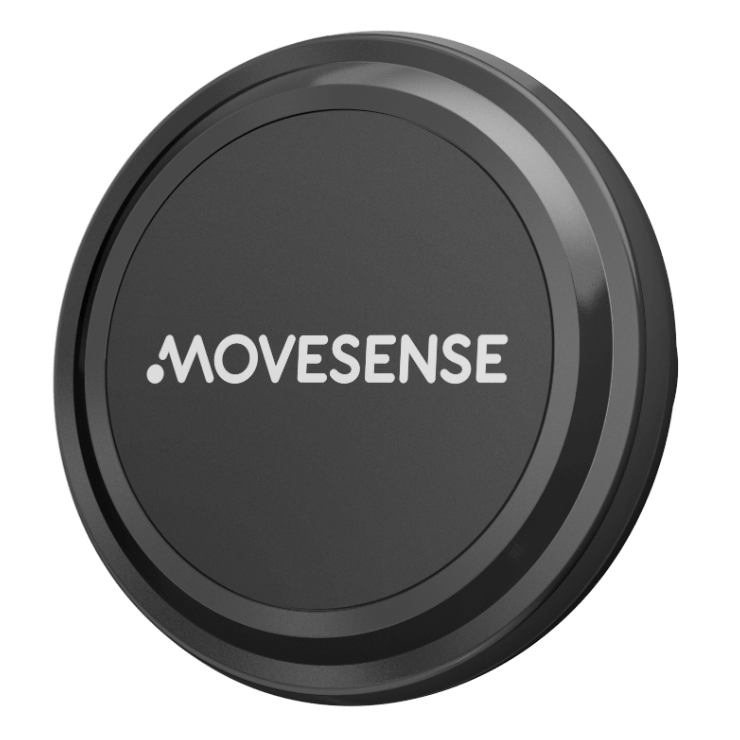
\includegraphics[width=0.9\textwidth]{content/3-Methods/movesense-persp-1000px.png}
    \caption{Front}
    \label{subfig:methods-movesense-sensor}
    \end{subfigure}
    \begin{subfigure}[b]{0.4\textwidth}
         \centering
         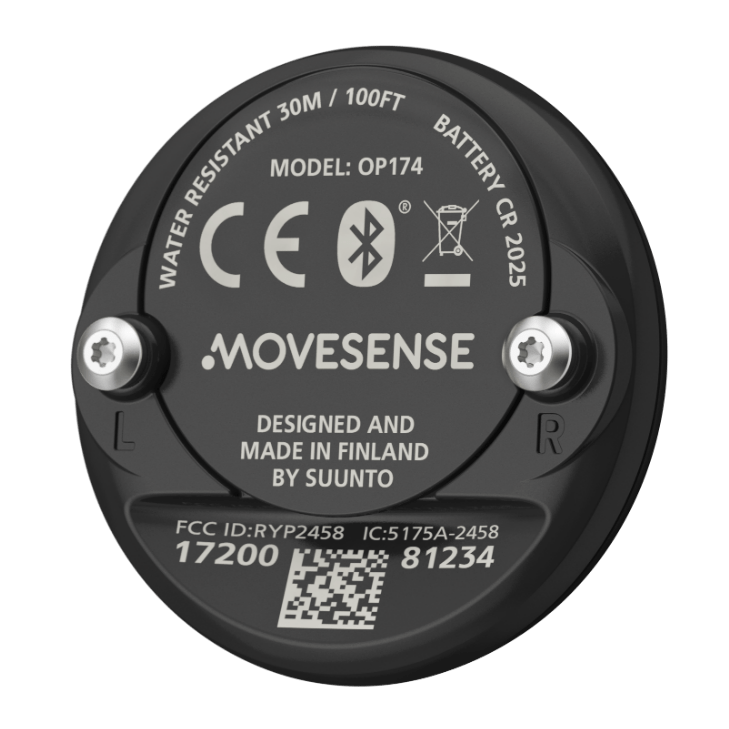
\includegraphics[width=0.9\textwidth]{content/3-Methods/Movesense-rear-1000px.png}
        \caption{Rear}
        \label{subfig:methods-movesense-rear}
    \end{subfigure}
    \caption[Movesense Wearable IMU]{Movesense Wearable IMU \cite{movesenseImg2019}}
    \label{fig:methods-movesense-sensor}
\end{figure}

Custom software can be installed allowing for bespoke setup of the device using the \acrfull{sdk} provided by Suunto. In this software device hardware is accessed through calls to the sensor \acrfull{api}. A custom program was produced that subscribed to the 100Hz \acrshort{marg} output, heart rate and temperature sensor. These were then transmitted over BLE to a android app for data logging. Further details on these steps are presented in subsequent sections.

The software also implemented power management, placing the sensors in a ultra-low power state when inactive, as detected by the accelerometer, for more than 10 minutes. The devices could then be woken again by pressing the rear contacts. This wake interrupt detection is a feature of the on board heart rate monitoring sensors.

The device's rear contact also act as mounting point for attaching the device to a wide variety of sensors. These include heart rate straps and Velcro strap. Five sensors were attached to each participant in the following locations: on the inside of both ankles using an elastic Velcro strap, on~each hip using a clothes/belt clip and across the chest using a heart rate strap. The location of the sensors was selected to give wide coverage of body movements while providing easy, secure and non-invasive attachment to minimize discomfort and disruption to natural movement. Figure~\ref{fig:methods-movesense-sensor-locations} shows a subject wearing the five sensors.

\begin{figure}[!hbt]
    \centering
    \includegraphics[width=0.4\textwidth]{example-image-a}
    \caption{Movesense sensor attachment locations}
    \label{fig:methods-movesense-sensor-locations}
\end{figure}

% How is sensor data transmitted 
\subsubsection{BLE Data Transmission}
\label{subsection:methods-on-sensor-compression}
Data is transmitted wireless using the built in \acrfull{ble} transceiver in the Movesense to a connected smartphone. The process for preparing the sensor data for transmission is presented below.

A custom GATT service was created that allows data packed to be pushed to a connected smartphone. Data pushing is done using the \acrshort{ble} notify mechanism. Data streaming starts when a notify state is set on the \acrshort{ble} characteristic. It stops again when the notify state is cleared. Only enters the high power draw streaming state when recording.

Two limits restrict the data rate that the sensor can transmit. The maximum individual packet size that can be transmitted by the Movesense device is 155 bytes long. There is also a maximum practical transmission rate of less than 15Hz, due to requirements for transmission concurrently from five sensors. The transmission limit require that to achieve a 100Hz sample rate multiple \acrshort{imu} samples are transmitted per packet.

\acrshort{imu} data from the sensor is provided as a 32-bit floating point number. Each sample of the three axis for each of the three sensors requires 36 bytes. At full size only four samples can be packed within the limit for a single BLE transmission. Therefore compression of the data is required.

Compressing the data to 16-bit fixed point signed integer values allow for eight packets of data to be transmitted concurrently. The compression is achieved by multiplying the original value by a scaling factor before typecast to a int-16. This retains the sub-decimal accuracy while allowing for sufficient compression. Table \ref{tab:methods-imu-data-compression-factors} presents the sensor ranges, scaling factors and resultant accuracy of each sensor. As 16-bit integer values have a maximum range of $-32,768$ to $32,767$ clipping would occur if the scaled value of the sensors exceeds this. The scaling factor was therefore chosen as a balance between accuracy and output range with the output range requirement calculated experimentally.

\begin{table}[!hbt]
    \centering
    \caption[Sensor compression scaling factors and accuracies]{Sensor compression scaling factors and accuracies. G --- Force of Gravity, DPS --- Degrees per Second, $\mu T$ --- MicroTesla}
    \label{tab:methods-imu-data-compression-factors}
    
    \begin{tabular}{l|ccc}
         \textbf{Sensor} & \textbf{Sensor Range} & \textbf{Scaling Factor} & \textbf{Accuracy} \\
         \hline
         Acceleromenter & $\pm16 G$ & $256$ & $\pm0.039 G$  \\
         Gyroscope & $\pm2000 DPS$ & $32$ & $\pm0.031 DPS$  \\
         Magnetometer & $\pm5000\mu T$ & $1$ & $\pm1\mu T$
    \end{tabular}
\end{table}

Once compressed 8 IMU samples fit within one packet leaving 11 bytes available. A timestamp based on the internal sensor clock is transmitted as a 32-bit unsigned integer. Six further bytes is populated with the temperature, heart rate and R-R interval recording from the sensor. These were added for future use. As these values are only provided by the sensor on a change in value the remaining byte is used as a update flag for each field. Figure \ref{fig:methods-ble-packet-structure} illustrates the full 155 byte transmission packet.

\begin{figure}[!hbt]
    \centering
    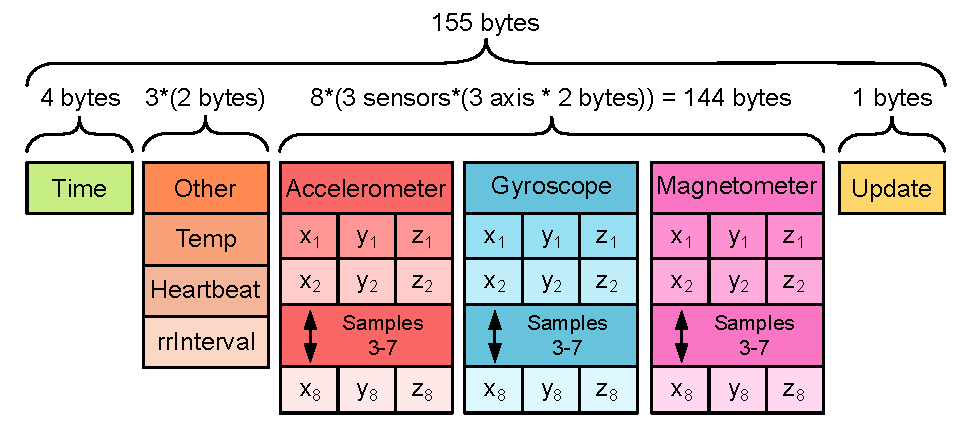
\includegraphics[width=0.9\textwidth]{content/3-Methods/BLE_Bytes_Packets.pdf}
    \caption[Movesense data packet structure]{Movesense Bluetooth Low Energy characteristic transmission packet structure}
    \label{fig:methods-ble-packet-structure}
\end{figure}

\subsection{Android App}
The \acrshort{ble} data stream is received by a smart phone held by the participant. This serves three purposes: to save the sensor data, to annotate the current activity, and to share annotated data with the researcher. These three steps are described in more detail below. 

In recording mode three services run; \acrfull{ui} and \acrshort{ble} and file background services. The \acrshort{ui} service commands the \acrshort{ble} and File services based on user input and also relays information from the two background services to the user. This information includes errors with the sensors and recording statistics. An illustration of the interactions between each aspect of the app is shown in Figure \ref{fig:methods-android-app}.

\begin{figure}[!hbt]
    \centering
    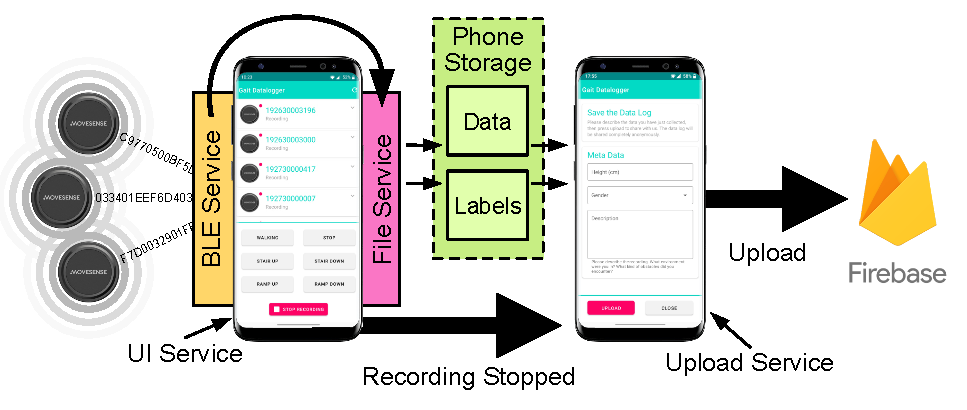
\includegraphics[width=0.9\textwidth]{content/3-Methods/Android_App.pdf}
    \caption{Data-logging Android App}
    \label{fig:methods-android-app}
\end{figure}

\subsubsection{User Interface}
The user interface of the app is intentionally simple requiring minimal instruction to use. The interface is handled by the \acrshort{ui} service. A \acrshort{ble} connection is automatically established with any 'on' sensor that is detected during a \acrshort{ble} device scan when the app opens. If not all sensors are found this search can be repeated.

During recording a series of buttons at the bottom of android app are used to annotate the current activities. Each time a button is pressed the file service records both the name of the button and the phone timestamp to a label file.

Once recording had finished the user is presented with an upload screen allowing metadata to be added and data to be shared with researchers.

\subsubsection{Saving Sensor Data}
The android app is primarily responsible for forming a \acrshort{ble} connection to each sensor and saving the sensor data stream to a file that could be interpreted later. This \acrshort{ble} connection is managed by a background \acrshort{ble} service in the app.

Record is started by the subject pressing the record button. The app then sets the notify state on each device starting data streaming. Received data is passed from the BLE service to the file saving service. This service creates plain text files locally on the phone. Each message of data is saved on a new line in the file along with the phone time stamp and MAC address of the sensor. The data message is saved as a hexadecimal representation of the received binary data string. All sensors are saved together in a single file with each line representing a received BLE data message.

The saved file can then be shared anonymously with the researchers using Google's Firebase cloud services. This uploads the files saved to the phone to google's cloud servers for later retrieval by researchers.

%------------------------------------------------------------%
\section{Data Collection}
\label{sec:methods-data-collection}
First hand data

Introduction and purpose of data collections

%Ethics Approval
The study received ethical approval from the University of Bath Research Ethics Approval Committee for Health (REACH), reference \textit{EP 19/20 003}.

\subsection{Activities}
What activities are we recording. What is the justification for this split

% The following activities were selected, Walking (W), Stair Ascent (SA), Stair Descent (SD), Ramp Ascent (RA), Ramp~Descent (RD) and Stopped (S). Labarri\`ere et al. identified these as the most commonly investigated and they require no equipment or skill to perform~\cite{Labarriere2020}. 

% Pictures showing the variety of terrain %
\begin{figure}[!hbt]
     \centering
     \begin{subfigure}[b]{\textwidth}
         \centering
         \begin{subfigure}[b]{0.32\textwidth}
             \centering
             \includegraphics[width=\textwidth]{example-image-a}
        \end{subfigure}
        \hfill
         \begin{subfigure}[b]{0.32\textwidth}
             \centering
             \includegraphics[width=\textwidth]{example-image-b}
        \end{subfigure}
        \hfill
        \begin{subfigure}[b]{0.32\textwidth}
             \centering
             \includegraphics[width=\textwidth]{example-image-c}
        \end{subfigure}
        \caption{Walking}
        \label{fig:methods-flat-example}
      \end{subfigure}
      \newline
      
      \begin{subfigure}[b]{\textwidth}
         \centering
         \begin{subfigure}[b]{0.32\textwidth}
             \centering
             \includegraphics[width=\textwidth]{example-image-a}
        \end{subfigure}
        \hfill
         \begin{subfigure}[b]{0.32\textwidth}
             \centering
             \includegraphics[width=\textwidth]{example-image-b}
        \end{subfigure}
        \hfill
        \begin{subfigure}[b]{0.32\textwidth}
             \centering
             \includegraphics[width=\textwidth]{example-image-c}
        \end{subfigure}
        \caption{Stairs}
        \label{fig:methods-stair-example}
      \end{subfigure}
      \newline
      
      \begin{subfigure}[b]{\textwidth}
         \centering
         \begin{subfigure}[b]{0.32\textwidth}
             \centering
             \includegraphics[width=\textwidth]{example-image-a}
        \end{subfigure}
        \hfill
         \begin{subfigure}[b]{0.32\textwidth}
             \centering
             \includegraphics[width=\textwidth]{example-image-b}
        \end{subfigure}
        \hfill
        \begin{subfigure}[b]{0.32\textwidth}
             \centering
             \includegraphics[width=\textwidth]{example-image-c}
        \end{subfigure}
        \caption{Ramp/Hill}
        \label{fig:methods-ramp-example}
      \end{subfigure}
    \caption{Example of data recording environments}
    \label{fig:three graphs}
\end{figure}


\subsection{Recording Procedure}
How were the subjects instructed to label data - press at first HS on new activity
% Does this belong here - probably covered by each individual section

% Study subjects were provided with instructions on how to use the sensing equipment, and the activity classes, then~allowed to record as they wished. Participants were instructed to walk around a varied environment with the sensor on while labelling the six activity classes. No~further instructions on how the recording should be conducted were provided.

\subsection{Data-Set Summary} %Should this be part of the materials section?
A brief summary of the data collected over the course of this research is presented in this section. This is followed by a short discussion about the quality of the data.

Data was collected in three phases:
\begin{itemize}
    \item Large number of non-amputee participants - limited data per participant
    \item Small number of non-amputee participants - extensive data per participant
    \item Data from amputees
\end{itemize}
Within this section a brief summary of the data collected is presented.

The first phase of data collection involves collecting a data with a focus of collecting from a broad range of individuals in different environments. Table \ref{tab:methods-phase-1-data-summary} contains a summary of the data collected during the first phase of data collection. Data was collected from twenty-two participants of a wide variety of age (mean 29, std 10), gender (17 male, 5 female), and physique.
\newcolumntype{Y}{>{\centering\arraybackslash}X}
\begin{table}[!hbt]
    \centering
    \caption[Data samples of non-amputee data collected during the first phase of data collection]{Summary of non-amputee data collected during the first phase of data collection.}
    %W---Walking, RA---Ramp Ascent, RD---Ramp Descent, SA---Stair Ascent, SD---Stair Descent, S---Stopped
    \begin{tabularx}{\textwidth}{c|YYYYYY}
       \textbf{Subject ID} & \textbf{W} & \textbf{RA} & \textbf{RD} & \textbf{SA} & \textbf{SD} & \textbf{S} \\
       \hline
       01 & 1111 & 2222 & 3333 & 4444 & 5555 & 6666 \\
       02 & 1111 & 2222 & 3333 & 4444 & 5555 & 6666 \\
       03 & 1111 & 2222 & 3333 & 4444 & 5555 & 6666 \\
       04 & 1111 & 2222 & 3333 & 4444 & 5555 & 6666 \\
       05 & 1111 & 2222 & 3333 & 4444 & 5555 & 6666 \\
       06 & 1111 & 2222 & 3333 & 4444 & 5555 & 6666 \\
       07 & 1111 & 2222 & 3333 & 4444 & 5555 & 6666 \\
       08 & 1111 & 2222 & 3333 & 4444 & 5555 & 6666 \\
       09 & 1111 & 2222 & 3333 & 4444 & 5555 & 6666 \\
       10 & 1111 & 2222 & 3333 & 4444 & 5555 & 6666 \\
       11 & 1111 & 2222 & 3333 & 4444 & 5555 & 6666 \\
       12 & 1111 & 2222 & 3333 & 4444 & 5555 & 6666 \\
       13 & 1111 & 2222 & 3333 & 4444 & 5555 & 6666 \\
       14 & 1111 & 2222 & 3333 & 4444 & 5555 & 6666 \\
       15 & 1111 & 2222 & 3333 & 4444 & 5555 & 6666 \\
       16 & 1111 & 2222 & 3333 & 4444 & 5555 & 6666 \\
       17 & 1111 & 2222 & 3333 & 4444 & 5555 & 6666 \\
       18 & 1111 & 2222 & 3333 & 4444 & 5555 & 6666 \\
       19 & 1111 & 2222 & 3333 & 4444 & 5555 & 6666 \\
       20 & 1111 & 2222 & 3333 & 4444 & 5555 & 6666 \\
       21 & 1111 & 2222 & 3333 & 4444 & 5555 & 6666 \\
       22 & 1111 & 2222 & 3333 & 4444 & 5555 & 6666 \\
    \end{tabularx}
    \label{tab:methods-phase-1-data-summary}
\end{table}

The second phase of data collection involved the collection of data from a much smaller number of individuals but with a focus on collecting at least seven minutes of data for each activity. Table \ref{tab:methods-phase-2-data-summary} show a summary of the data collected during the second phase. Data was collected from two subjects, one male of age 27, and one female of age 26.
\begin{table}[!hbt]
    \centering
    \caption[Data samples of non-amputee data collected during the second phase of data collection]{Data samples of non-amputee data collected during the second phase of data collection}
    \begin{tabularx}{\textwidth}{c|YYYYYY}
       \textbf{Subject ID} & \textbf{W} & \textbf{RA} & \textbf{RD} & \textbf{SA} & \textbf{SD} & \textbf{S} \\
       \hline
       01 & 1111 & 2222 & 3333 & 4444 & 5555 & 6666 \\
       09 & 1111 & 2222 & 3333 & 4444 & 5555 & 6666 \\
    \end{tabularx}
    \label{tab:methods-phase-2-data-summary}
\end{table}

% Third round of data collection
The third range of data collection is amputee data, this involved collecting data with the recording data procedures. Table \ref{tab:methods-phase-3-data-summary} contains a summary of the first hand data collected during this phase. The data was for one trans-tibial amputee.
% Amputee data
\begin{table}[!hbt]
    \centering
    \caption[Data samples of first hand amputee data collected during the third phase of data collection]{Data samples of first hand amputee data collected during the third phase of data collection.}
    \begin{tabularx}{\textwidth}{c|YYYYYY}
       \textbf{Subject ID} & \textbf{W} & \textbf{RA} & \textbf{RD} & \textbf{SA} & \textbf{SD} & \textbf{S} \\
       \hline
       A1 & 1111 & 2222 & 3333 & 4444 & 5555 & 6666 \\
    \end{tabularx}
    \label{tab:methods-phase-3-data-summary}
\end{table}

Additional data was also supplied by the Bio-Mechanics lab of the University of Bath and Blatchford Ltd. Table \ref{tab:methods-second-hand-amputee-data} contains a summary of the additional data obtained during this phase. The data was for \hl{x} trans-tibial and \hl{y} trans-femoral amputees.
% bio-mechanics data of amputee - recap what's different about this data
\begin{table}[!hbt]
    \centering
    \caption[Data samples for other amputee data obtained]{Data samples for other amputee data obtained.}
    \begin{tabularx}{\textwidth}{c|YYYYYY}
       \textbf{Subject ID} & \textbf{W} & \textbf{RA} & \textbf{RD} & \textbf{SA} & \textbf{SD} & \textbf{S} \\
       \hline
       A2 & 1111 & 2222 & 3333 & 4444 & 5555 & 6666 \\
    \end{tabularx}

    \label{tab:methods-second-hand-amputee-data}
\end{table}


What is unique about our data set
\begin{itemize}
    \item Unsupervised (no researcher bias in activity pattern) - subject Provided with sensors, app and basic instructions of how to setup and label data
    \item Wide range of different natural environments and terrain
    \item Large number of people
\end{itemize}

Issues with the data
\begin{itemize}
    \item Poorly distributed classes - real life distribution of activities is not even. Walking and hills/ramps are far more prevalent than stairs - % TODO add in percentage of each activity type for the overall data set and a mean/std per participant 
    \item Transition between activities is inconsistent and only labelled at one point
    \item Label noise
    \item Different amounts of data for different participants
\end{itemize}

%------------------------------------------------------------------%
\section{Data Post-Processing}
The raw saved data must be transformed in order that it can be used in a machine learning environment. Within this sections the methods used to accomplish this transformation are detailed.

% Terminology
The data collected can be described by the following hierarchical structure shown in Figure \ref{fig:methods-data-hierachy}.For each participant a series of data recordings are collected. Each recordings potentially contain different distributions of activities and in different environments. The recording contains a series of activities live annotated by the subject. Each continuous period of one activity label is an episode of data. So a recording is made up of a series of contiguous episodes of data. The period at the end of one episode and start of the next is the transition period between activities. This is represented as a discrete change but in reality would be a smooth easing between locomotive modes.

\begin{figure}[!hbt]
    \centering
    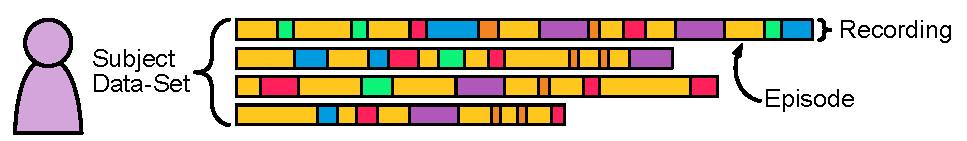
\includegraphics[width=0.9\textwidth]{content/3-Methods/Data_Terminology.pdf}
    \caption{Hierarchical structure of the data recordings and terminology}
    \label{fig:methods-data-hierachy}
\end{figure}

%Issues with the data

    
To prepare the data for \acrshort{ml} and address issues with the data two \acrfull{etl} scripts were written. An \acrshort{etl} is a common technique in data science for copying data from one or more source to a new destination which requires a different representation of the data. A \acrshort{etl} script written in Matlab is used to transform the sensor data from it's saved form to csv files that could easily be imported into a Python. A second \acrshort{etl} script in python then prepare the data for loading into a machine learning environment. A more detailed description of these two scripts is presented in Sections \ref{subsec:sensor-ETL} and \ref{subsec:ML-ETL}

\subsection{Sensor Data ETL}
\label{subsec:sensor-ETL}
The sensor data \acrshort{etl} script transforms the raw saved sensor data into .csv tables that are easily importable into python. Each step of the \acrshort{etl} is described below. The overall process is illustrated in Figure \ref{fig:methods_sensor_ETL}.

\begin{figure}[!hbt]
    \centering
    \includegraphics[width=0.4\textwidth]{example-image-a}
    \caption{Flow Diagram of Sensor Data \acrshort{etl} process}
    \label{fig:methods_sensor_ETL}
\end{figure}

\subsubsection{Extract} % Extract - retrieving data from source
Data is saved in individual directory for each participant and a sub-directory for each recording session. Within each sub-directory three files are store, a data file, label file and meta-data file. The three files contain the following:
\begin{itemize}
    \item \textbf{Data File} -- Hexadecimal encoded binary sensor data along with the mobile phone timestamp at which it was received.
    \item \textbf{Label File} -- Plain text activity labels with timestamps of the activity start (the point at which the app button was pressed)
    \item \textbf{Meta File} -- Notes about the recording including the participant height, gender and a brief unstructured description of the recording.
\end{itemize}

Each sub-directory is opened and processed one at a time in no specified order.

\subsubsection{Transform}
% Transform
The sensor data is store as a Hexadecimal string, with each two characters representing one byte of the transmission string from the sensors. The first operation is converting each pair of characters back into it's original binary value. Then sets of binary values are typecast to integer values before scaling them back into there original 32-bit floating point representation. This is the reverse of the on sensor conversion described in Section \ref{subsection:methods-on-sensor-compression}.

Each line of sensor data contains the Physical/MAC address of the sensor. This is used to split the single file of data into individual sensors. Before combining the individual sensors into a single data table any inconsistency between the devices needs to be accounted for.

The senors do not have on-board real-time clocks the sensor timestamp is based upon their internal clock oscillator. There is sufficient variation between these that clock drift between sensors must be accounted for. To calculate a correction for the long term drift the message timestamp is compared to the smart phone clock. This drift is assumed to be linear therefore a linear regression can be calculated to determine a corrective factor. Figure \ref{fig:methods-clock-drift-correction} shows examples of drift correction. % \hl{}

\begin{figure}[!hbt]
    \centering
    \includegraphics[width=0.4\textwidth]{example-image-a}
    \caption{Example of sensor clock drift correction}
    \label{fig:methods-clock-drift-correction}
\end{figure}

Each data packet contains eight sensors readings, but only one timestamp. Therefore the timestamps for the each individual reading needs to be augmented.

Finally the data is re-sampled to exactly 100Hz to ensure data for each sensors aligns correctly. This was necessary as due to inconsistent sensor clocks the actual device sample rate varies. Re-sampled is performed using the built in Matlab re-sampling function using a spline function to calculate the interpolated value.At this point the individual sensors can be combine into a single data table.

\hl{Normalisation has been shown to improve the performance of ML models}. \cite{} % TODO: find citation
This is performed on a per recording basis maintaining the changes in magnitude that occur when changing between activities. The values for scaling and offset would need to specified on a per user basis for a physical system.

The last step is applying activity labels to the data table. The data labels recorded in the label file are aligned to the recorded data with each row given a label based on the last activity row.

\subsubsection{Load}
Two saving options were employed:
\begin{itemize}
    \item Saving the complete recording as a single file
    \item Splitting the recording up into different files for each episode of an activity
\end{itemize}

The data tables are exported as \acrfull{csv} files, with the \acrshort{csv} files for each participant stored in separate folders. Basic statistics about each file are also generated, including number of samples of each activity and step count.

%--------------------------------------------%
\subsection{Machine Learning ETL}
\label{subsec:ML-ETL}
The second ETL script ingests the \acrshort{csv} data files previously generated and converts and prepares them for loading into a Tensorflow machine learning environment. Tensorflow requires three sets of data, train, test, and validation, each presented as a set of data windows along with a corresponding model output. The \acrshort{etl} script is written in python 3.8. Within this section the process for doing this is presented. A flow diagram of the \acrshort{etl} process is shown in Figure \ref{fig:methods_ml_ETL}.

\begin{figure}[!hbt]
    \centering
    \includegraphics[width=0.4\textwidth]{example-image-a}
    \caption{Flow Diagram of Machine Learning Ingest \acrshort{etl} process}
    \label{fig:methods_ml_ETL}
\end{figure}

% Export
\subsubsection{Extract}
The extract process starts by importing the \acrshort{csv} files using the Python library Pandas. Using Pandas the \acrshort{csv} data is loaded into Pandas data tables and stored against it's associated participant and where applicable activity.

The \acrshort{etl} script also accepts a set of \acrshort{yaml} parameter files. Within these files the parameters for configuring the various transformations are stored. This allow experiments to be replaced quickly as the \acrshort{yaml} files can be stored with the input data and results. The \acrshort{etl} script also supports a \acrshort{yaml} file that specifies a range of values of a single or multiple parameters to test. This allows the \acrshort{etl} script to implement hyper-parameter sweeping.


\subsubsection{Transform -- Data Division}
%The data set was divided into two groups for test and training. The training set was used during the learning process with the test set reserved for evaluating the performance of unseen data. The test set was a variation of Leave One Out Cross-Validation (LOOXV). LOOXV involves training and analyzing the model multiple times with different excluded individuals, the results are then combined to improve statistical certainty. For this paper four/five subjects were excluded each time with analysis repeated five time, meaning each subject was excluded once. The training set contains the remaining subjects, with 30% of the data used as a validation set. Figure 9 provides an illustration of how the data is divided between the three data sets.

%To balance the data set, both the training and test sets were adjusted by removing data so that no class contained more than 50\% more samples than any another. This re-balancing was undertaken carefully so that during validation splitting the balance was maintained. A class weight input was used to bias the training to further balance the class labels.

%The continuous sensor data was segmented using sliding windows. Between the start of each window, an offset of five samples was used. This offset was set empirically to give the model a wide range of data windows position without slowing down learning from an unnecessarily large training set. The output label for each window was set as the recorded ground truth at the end of the window. Classification labels were presented using one-hot encoding.


What are the issues with our data set - primarily that it is poorly distributed. Can be fixed by truncating the dataset or by biasing the training algorithm (class weights).

Aims of division - cross validation + maximise use of relatively small available data / fix issues with the dataset.

Split into training, validation, test. Recap the needs of each of these datasets. Training is as broad a set of data as possible. Validation is a set data drawn out of the training set used to evaluate the training performance. Test should be an independent set of data with the same distribution as the training set. It must be unseen to the training algorithm.

Two methods have been used for dividing the data. The first splits the data by test subject, the second splits the data by activity episodes.

\paragraph{Per Participant Division}
\label{par:methods-per-participant-division}
Split on a per participant basis - natural division point for a group of people

Shuffled to provide a large number of different training and test sets

Limitations of this method
 - How did we accommodate different amounts of data per participant
 
Figure \ref{fig:methods-per-participant-division}
 
 \begin{figure}[!hbt]
     \centering
     \includegraphics[width=0.6\textwidth]{example-image-a}
     \caption{Per-participant data division}
     \label{fig:methods-per-participant-division}
 \end{figure}

\paragraph{Per Episode Division}
\label{par:methods-per-episode-division}
Can't easily split up data per participants due to poor distribution of classes. 

Figure \ref{fig:methods-per-episode-data-division} illustrates the process of forming the three data sets.
For experiments where only an individual participant is available split bases on 'episodes' of data

Episodes are all different lengths so how were episodes combined into test and training sets
    - combine episodes until a threshold is reached. Use remaining data as test set

Limitations of this method
 - Can end up with similar episodes in test and training (data shuffled and cross validation repeated multiple times)
 - Removes transitions from the data set (data is cleaner)
 
 Talk about under/over/mislabelling (Particularly around transitions). How did we account for these? Figure \ref{fig:methods-per-episode-data-division}
 
 \begin{figure}[!hbt]
     \centering
     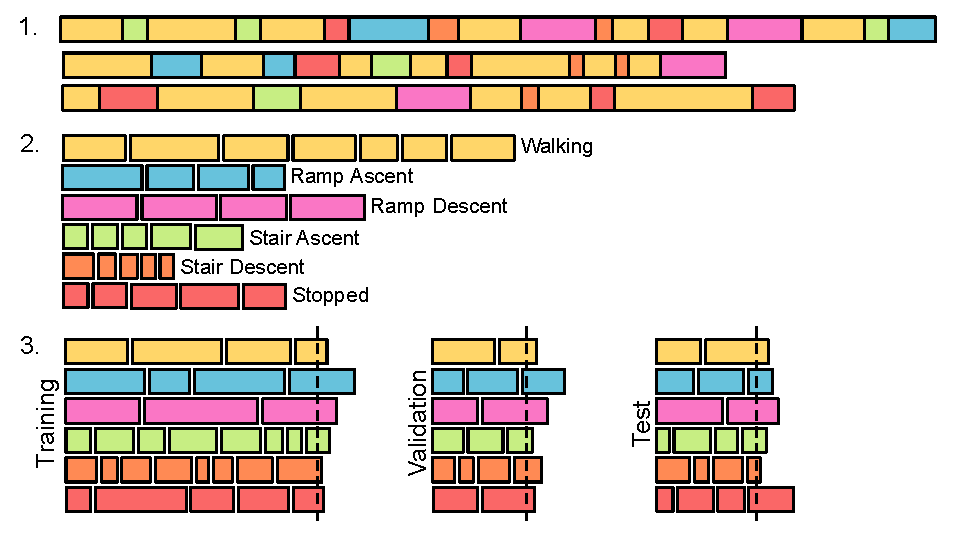
\includegraphics[width=0.9\textwidth]{content/3-Methods/Episode_Division.pdf}
     \caption[Per-episode data division]{Per-episode data division. Step 1 -- All data files for a participant are loaded and labeled. Step 2 -- Episodes of the same activity are grouped together. Step 3 -- Training, Validation and Test sets are formed by stacking episodes until a threshold is reached.}
     \label{fig:methods-per-episode-data-division}
 \end{figure}
 
 
\subsubsection{Transform -- Data Windowing}
The \acrshort{yaml} setup file specify the columns of data that are required, for example \textit{right-ankle-gyro-y}. The data columns specified are extracted from the Pandas data tables with the remaining data columns discarded.

To generate the data windows rows of data equal to the specified window size are selected and copied to form new Pandas data tables. This starts at the beginning of the data table with the starting index incremented forward by a specified step size for each new window. This results in a set of overlapping windows. Figure \ref{fig:methods-data-window-generation} illustrates the data window generation.

\begin{figure}[!hbt]
    \centering
    \includegraphics[width=0.6\textwidth]{example-image-a}
    \caption{Overlapping data window generation}
    \label{fig:methods-data-window-generation}
\end{figure}

The activity labels must be provided in the same output scheme as the \acrshort{ml} model, for classification format called a one-hot encoding in used. This gives each class a separate output with the classification given to the output with the highest value. The activity labels will be presented as an array of length equal to the number of activities. Each element of the array represents one of the activity classes. The class the label represents in encoded by setting the corresponding array element to a value of one.

%In Human Activity Recognition datasets, we note that the samples produced by the same subjects are likely to be correlated due to diverse factors. Hence, k-fold cross validation may overestimate the performance of activity recognizers, in particular when overlapping sliding windows are used. In this paper, we in- vestigate the effect of Subject Cross Validation on the performance of Human Activity Recognition, both with non-overlapping and with overlapping sliding windows. Results show that k-fold cross validation artificially increases the performance of recognizers by about 10\%, and even by 16\% when overlapping windows are used. In addition, we do not observe any performance gain from the use of overlapping windows. We conclude that Human Activity Recog- nition systems should be evaluated by Subject Cross Validation, and that overlapping windows are not worth their extra computational cost.\cite{Dehghani2019}


\subsubsection{Load}
Push into Tensorflow model

Group weights?


%------------------------------------------------------------------%
\section{Machine Learning Methods}
The central challenge in machine learning is that it our algorithm must perform well on new, previously unseen inputs. The ability to perform well on previously unobserved inputs is called generalisation.
What separates machine learning from optimisation is that we want the generalisation error to below as well as the training error.\cite{Goodfellow2015}

\subsection{Model Setup}
Python 3.7
Tensorflow 2.1
Computer specs

% Two different model architectures were developed, a simplified model with a single information path for investigating LSTM internal behavior; and a full complexity practical model based on the architecture presented by Murad et al. [11] for investigating hyperparameter sensitivities. This design was previously discussed in Section 2.2. For both architectures input data is fed directly into the first LSTM layer. For models with additional LSTM layer, the full output of the first LSTM layer is fed into input of the next layer and so on. The output from the final LSTM layer is fed into a fully connected dense layer followed by a ReLU classifier. For the simplified model the LSTM output is the last timestep only, for the full complexity model the full output of all timesteps is used. The size of the dense layer is equal to the number of outputs from the last LSTM layer. A one-hot classification output is used to encode the activity classes. Figure 8a,b show the architectures of the simplified and full complexity model, respectively.


\subsection{Model Training}
%The models were trained to minimize categorical cross-entropy. Model weights were initialized with a Golorot Uniform initializer [43] and optimized with an ADAM optimizer [44]. A dropout of 0.5 was used, selected experimentally, with network connections dropped between the last LSTM output and the dense classifier. During trained the full training dataset was used for each epoch, with data passed to the optimizer in mini batches of 2000 windows. At the end of each epoch the entire validation set was evaluated. Early stopping was used to prevent over-fitting, this stopped training when stagnation of validation cross-entropy loss was observed. Stagnation was identified by three consecutive losses of greater than the minimum previously seen. The model was trained on a PC with an AMD Ryzen 3600 CPU and a Nvidia Geforce RTX 2060 Super. Using GPU training, each epoch took approximately 10 s with between30 and 100 epochs required to train each model depending on the model size and the number of output classes.

hyper parameter sweeping

The test set - composed of examples coming from the same distribution as the training set, can be used to estimate generalisation error of a learner, after the learning process has completed.\cite{Goodfellow2015}

Training set is formed of data used 
Validation set is formed by part of the training set

The validation set error will underestimate the generalisation error, though typically by a smaller amount that the training error. The generalisation error may be estimated using the test set.\cite{Goodfellow2015}

\subsection{Performance analysis}
Accuracy

Confusion matrices
%Miss-classification will be analyzed using confusion matrices. A confusion matrix is a tabular representation of the performance of a classifier. Each cell is populated by a count of the ground truth against the classified output. This allows the accuracy of individual classes and confusion between classes to be assessed.

Precision - What proportion of positive identifications was actually correct? (A model that produces no false positives has a precision of 1.0.)

$p = \frac{TP}{TP + FP} $

Recall - What proportion of actual positives was identified correctly? (A model that produces no false negatives has a recall of 1.0.)

$r = \frac{TP}{TP + FN}$

F1-Score
% EOF

\chapter{Understanding LSTM Locomotion Mode Recognition Behaviour}
\label{chp:lstm-general}

\section{Introduction and Commentary}
% Where possible please ensure that the page numbers tie in with the rest of the thesis document, 
% where this is not possible, you should insert an extra page before the academic paper which shows 
% the citation details and gives the page numbers of the thesis that the academic paper covers.
Following the data collection, work began on developing a general-purpose \acrfull{lstm} network for classifying the locomotive mode of a previously unseen user. This involved work to understand how LSTM  networks can recognise different locomotive modes. Once completed, an article entitled ``Understanding LSTM Network Behaviour of IMU-Based Locomotion Mode Recognition for Applications in Prostheses and Wearables'' was submitted to the Journal Sensors. The paper was submitted as part of a call for papers on Machine Learning and Multimodal Sensing for Smart Wearable Assistive Robotics and published on the 10\textsuperscript{th} of February 2021.

The remainder of this chapter will be the presentation of the paper, followed by a short post-commentary. The paper is re-typeset to match the thesis. Page, section and reference numbering has been changed from the published copy.

%\newcommand\x{\value{page}}
 %The paper is presented as published and as such contains both the journal and thesis page numbering. The full paper covers thesis pages \the\numexpr\x+2\relax \ to \the\numexpr\x+24\relax.


\section*{Authorship and permissions}
% \newcommand{\backgoundColor}{0.871,0.918,0.965}
\newcommand{\backgoundColor}{1,1,1}
\newcommand{\boxColor}{0.95,0.95,0.95}
\begin{table}[H]
\caption{Statement of Authorship}
\hyphenpenalty=10000
\begin{tabularx}{\textwidth}{>{\raggedright}p{1.5in}X}
\hline
\rowcolor[rgb]{\backgoundColor}
\multicolumn{2}{l}{\textbf{This declaration concerns the article entitled:}}\\
\hline
\multicolumn{2}{p{0.9\textwidth}}{Understanding LSTM Network Behaviour of IMU-Based Locomotion Mode Recognition for Applications in Prostheses and Wearables} \\

\hline
\rowcolor[rgb]{\backgoundColor}
\multicolumn{2}{l}{\textbf{Publication status (tick one)}}  \\
\rowcolor[rgb]{\backgoundColor}
\multicolumn{2}{l}{\begin{tabular}{rcrcrcrcrc}
    \textbf\ {Draft} &{\cellcolor[rgb]{\boxColor}} \ &
    \textbf{\ Submitted} &{\cellcolor[rgb]{\boxColor}} \ &
    \textbf{\ In review} &{\cellcolor[rgb]{\boxColor}} \ &
    \textbf{\ Accepted} &{\cellcolor[rgb]{\boxColor}} \ &
    \textbf{\ Published} &{\cellcolor[rgb]{\boxColor}}X 
\end{tabular}}  \\
\rowcolor[rgb]{\backgoundColor}\multicolumn{2}{l}{} \\

% Publication details
\hline
{\cellcolor[rgb]{\backgoundColor}}\textbf{Publication details (reference)} & Sensors 2021, 21, 1264.

DOI: \href{https://doi.org/10.3390/s21041264}{10.3390/s21041264} 

Received: 23 December 2020, Accepted: 6 February 2021, Published: 10 February 2021\\


\hline
\rowcolor[rgb]{\backgoundColor}
\multicolumn{2}{l}{\textbf{Publication status (tick one)}} 

\\
\rowcolor[rgb]{\backgoundColor}
\multicolumn{2}{l}{\begin{tabular}{rcrc}
    \textbf{I hold the copyright} &{\cellcolor[rgb]{\boxColor}} \ &
    \textbf{\ Copyright is retained by the publisher, but} &{\cellcolor[rgb]{\boxColor}}X \\
    \textbf{for this material}& & \textbf{I have been given permission to replicate} & \\
    & & \textbf{ the material here} & \\
\end{tabular}}  \\
\rowcolor[rgb]{\backgoundColor}\multicolumn{2}{l}{} \\

\hline
{\cellcolor[rgb]{\backgoundColor}}\textbf{Candidate’s contribution to the paper (provide details, and also indicate as a percentage)} & The candidate predominantly executed the:

\textbf{Formulation of ideas: (95\%)}

The experiment and analysis methodology was conceived by Freddie Sherratt with supervision from Pejman Iravani

\textbf{Design of methodology: (95\%)}

The experiment and analysis methodology was conceived by Freddie Sherratt with supervision from Pejman Iravani

\textbf{Experimental work: (95\%)}

The experimental work was carried out entirely by Freddie Sherratt with supervision from Pejman Iravani

\textbf{Presentation of data in journal format: (95\%)}

The data presentation was carried out entirely by Freddie Sherratt with supervision from Pejman Iravani and Andrew Plummer\\

\hline
{\cellcolor[rgb]{\backgoundColor}}\textbf{Statement from Candidate} &
This paper reports on original research I conducted during the period of my Higher Degree by Research candidature.\\

\hline
{\cellcolor[rgb]{\backgoundColor}}\textbf{Signed} & Freddie Sherratt 
{\begin{tabular}{p{0.6in}ll}
     \ & {\cellcolor[rgb]{\backgoundColor}}\textbf{\ \ Date } & 4th March 2021 
\end{tabular}}\\
\hline
\end{tabularx}
\end{table}
\clearpage

% Paper
% \phantomsection
% \addtocounter{section}{1}
% \addcontentsline{toc}{section}{\arabic{chapter}.\arabic{section}~~~ Article: Understanding LSTM Network Behaviour of IMU-Based Locomotion Mode Recognition  for Applications in Prostheses and Wearables}


% This is the published PDF copy
% 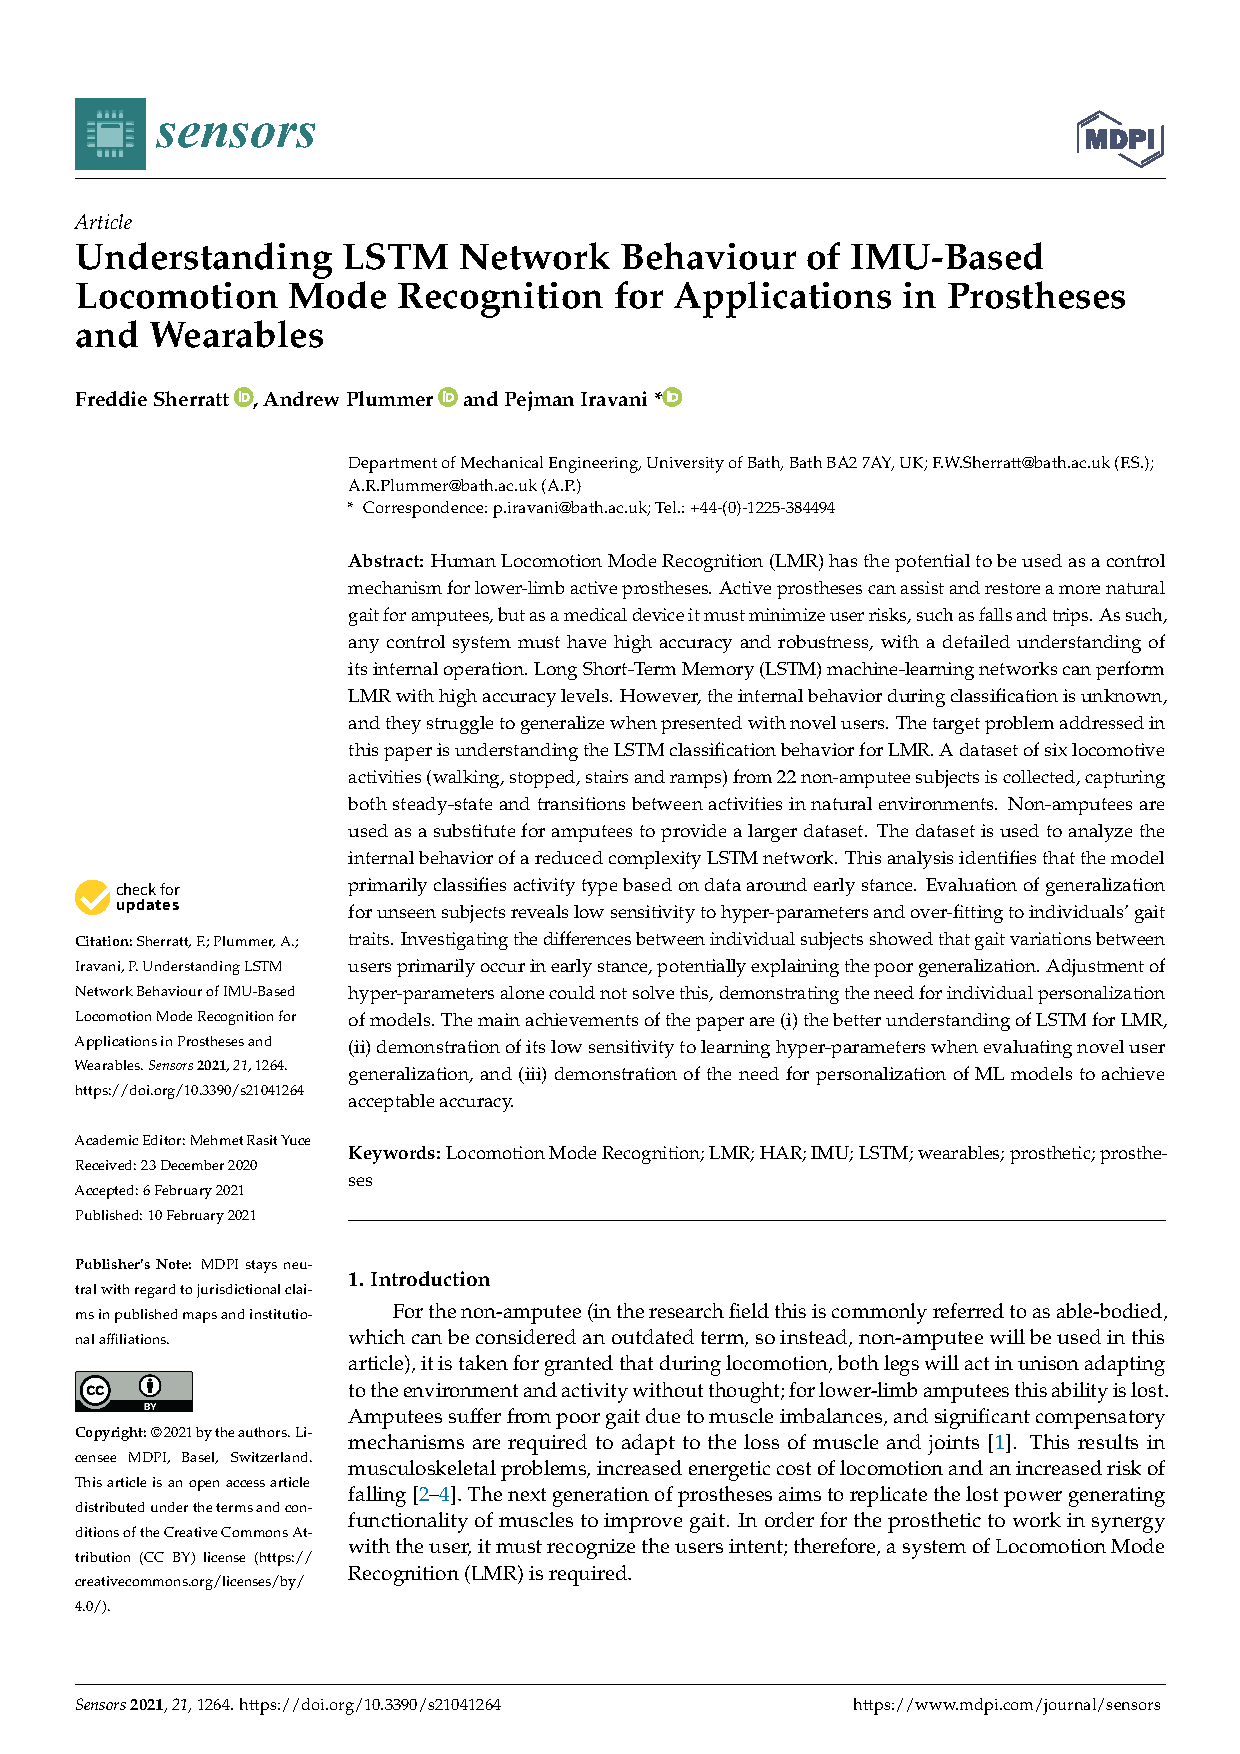
\includepdf[pages=-,scale=.83,offset=11mm 8mm,pagecommand={\thispagestyle{fancy}}, frame=false]{content/4-LSTM_Behaviour/sensors-21-01264-v2.pdf}

% This is a re-type setting of the paper
{\huge\textbf{Understanding LSTM Network Behaviour of IMU-Based Locomotion Mode Recognition for Applications in Prostheses and Wearables}\par}

Freddie Sherratt, Andrew Plummer and Pejman Iravani

Received: 23 December 2020; Accepted: 6 February 2021; Published: 10 February 2021

\textbf{Abstract:} Human \acrfull{lmr} has the potential to be used as a control mechanism for lower-limb active prostheses. Active prostheses can assist and restore a more natural gait for amputees, but as a medical device it must minimize user risks, such as falls and trips. As such, any control system must have high accuracy and robustness, with a detailed understanding of its internal operation. \acrfull{lstm} machine-learning networks can perform \acrshort{lmr} with high accuracy levels. However, the internal behavior during classification is unknown, and they struggle to generalize when presented with novel users. The target problem addressed in this paper is understanding the \acrshort{lstm} classification behavior for \acrshort{lmr}. A dataset of six locomotive activities (walking, stopped, stairs and ramps) from 22 non-amputee subjects is collected, capturing both steady-state and transitions between activities in natural environments. Non-amputees are used as a substitute for amputees to provide a larger dataset. The dataset is used to analyze the internal behavior of a reduced complexity \acrshort{lstm} network. This analysis identifies that the model primarily classifies activity type based on data around early stance. Evaluation of generalization for unseen subjects reveals low sensitivity to hyper-parameters and over-fitting to individuals’ gait traits. Investigating the differences between individual subjects showed that gait variations between users primarily occur in early stance, potentially explaining the poor generalization. Adjustment of hyper-parameters alone could not solve this, demonstrating the need for individual personalization of models. The main achievements of the paper are (i) the better understanding of \acrshort{lstm} for \acrshort{lmr}, (ii) demonstration of its low sensitivity to learning hyper-parameters when evaluating novel user generalization, and (iii) demonstration of the need for personalization of ML models to achieve acceptable accuracy.

\textbf{Keywords}: Locomotion Mode Recognition; LMR; HAR; IMU; LSTM; wearables; prosthetic; prostheses

\section{Introduction}
% Generic introduction to prostheses and the problems users face
For the non-amputee %MFPI: Footnote is not permitted in this journal, so we have moved it into the text, please confirm the whole text. please check all
(in the research field this is commonly referred to as able-bodied, which~can be considered an outdated term, so~instead, non-amputee will be used in this article), it~is taken for granted that during locomotion, both~legs will act in unison adapting to the environment and activity without thought; for lower-limb amputees this ability is lost. Amputees suffer from poor gait due to muscle imbalances, and~significant compensatory mechanisms are required to adapt to the loss of muscle and joints~\cite{Silverman2008}. This~results in musculoskeletal problems, increased energetic cost of locomotion and an increased risk of falling~\cite{Herr2012, Piazza2017, McDonald2018}. The~next generation of prostheses aims to replicate the lost power generating functionality of muscles to improve gait. In~order for the prosthetic to work in synergy with the user, it~must recognize the users intent; therefore, a~system of Locomotion Mode Recognition (LMR) is required.

% What existing solutions are there.
Several commercially available prostheses exist that actively adapt to the user intent, such~as Ottobock's Enpower BiOM~\cite{Enpower}, Blatchford's ElanIC~\cite{ElanIC} and \"Ossur's Proprio Foot~\cite{Proprio}. None~of these three provides more than basic functions, such~as maintaining dorsiflexion during leg swing to increase toe clearance and adjusting ankle resistance based on terrain. Only~the BiOM ankle offers powered assist in push-off, the~controller for this relies on hand-tuned heuristics control strategies~\cite{Montgomery2018}.   {The University of Bath with commercial partners has also been developing a next generastion powered prosthesis}~\cite{Yu2019}.

% Problems\Research gaps
Machine Learning (ML) offers the ability to significantly increase the sophistication of such systems, through understanding of a wide range of activities and personalization to individual characteristics, without specialist intervention~\cite{Labarriere2020}. As~classifying activities is temporal is nature, sequential ML networks, such~as Long Short-Term Memory (LSTM), are~a good fit. LSTM~networks have been demonstrated to be extremely capable at Human Activity Recognition (HAR), accurately identifying actions from locomotive actions, such~as Walking, Running and Stairs~\cite{Murad2017}, to~Hip-Hop dance moves~\cite{Samprita2020}. However, little is known of their understanding internal behavior during these tasks. For~a medical device, such~as a prosthetic, both~a high levels of accuracy and detailed knowledge of internal network operation is required.

% How we are going about answering the research gap/question
This paper explores in detail the operation and performance of LSTM networks for LMR using both seen and novel users. Data~from non-amputee participants is used as a substitute for amputee data as it allows for a much larger and more varied data set while minimizing risk to subjects. This~is then used to investigate the internal operation on a simplified LSTM network. The~effects of hyper-parameters on the generalization performance of a practical LSTM network are then investigated. Finally, changes to the model are investigated to try and improve its performance for novel users. 

% What are the major contributions of this paper
The major contributions of this work are as follows:
\begin{enumerate}
\item Methodology for the collection of a large self-supervised data set of human locomotion data in a natural environment.
\item Provide an insight into the behavior of an LSTM LMR model, and~the performance effects of hyper-parameter selection.
\item Investigation of hyper-parameter sensitivities in an LSTM network and their effect on classification accuracy and generalization to novel user.
\item Demonstration of the need for personalization techniques to account for individual gait traits.
\end{enumerate}

The remainder of this paper is organized as follows; First background theory on the Human Gait Cycle and LSTMs is presented in Section \ref{sec:theory}. Section \ref{sec:related_work} contains Related work followed by Section \ref{sec:materials_and_methdology}---Materials and Methodology, describing the data collection process and setup of the ML environment. The~following Sections  \ref{sec:simplified_model} and \ref{sec:full_complexity}, detail the experiments undertaken, investigating LSTM behavior, and~hyper-parameter sensitivities, respectively. These each follow the same structure with an introduction to the experiment, analysis methodology, then~results and discussions. The~remaining two sections, Sections \ref{sec:discussion} and \ref{sec:conclusion}, contain discussion and conclusions.

\section{Human Gait and Machine-Learning Fundamentals}
\label{sec:theory}
Within this section fundamental theory of the human gait cycle, and~Recurrent Neural Networks (RNN) and LSTMs is presented.

\subsection{Locomotion Mode Recognition and the Human Gait Cycle}

Human gait is a cyclic process that can be delineated by key events. A~gait cycle is defined by two successive Initial Contact (IC) events (the point at which the foot contacts the ground) of the same limb. As~this is normally the heel, it~is often referred to as Heel Strike (HS). Conversely, the~point when the foot leaves the ground is referred to as Toe Off (TO). These two events are used to subdivide the gait into two phases; stance---when the foot is on the ground, and~swing when not. A~diagram showing these events and their location in the gait cycles is shown in Figure~\ref{fig:gait_cycle}.

\begin{figure}[!hbt]
    \centering
    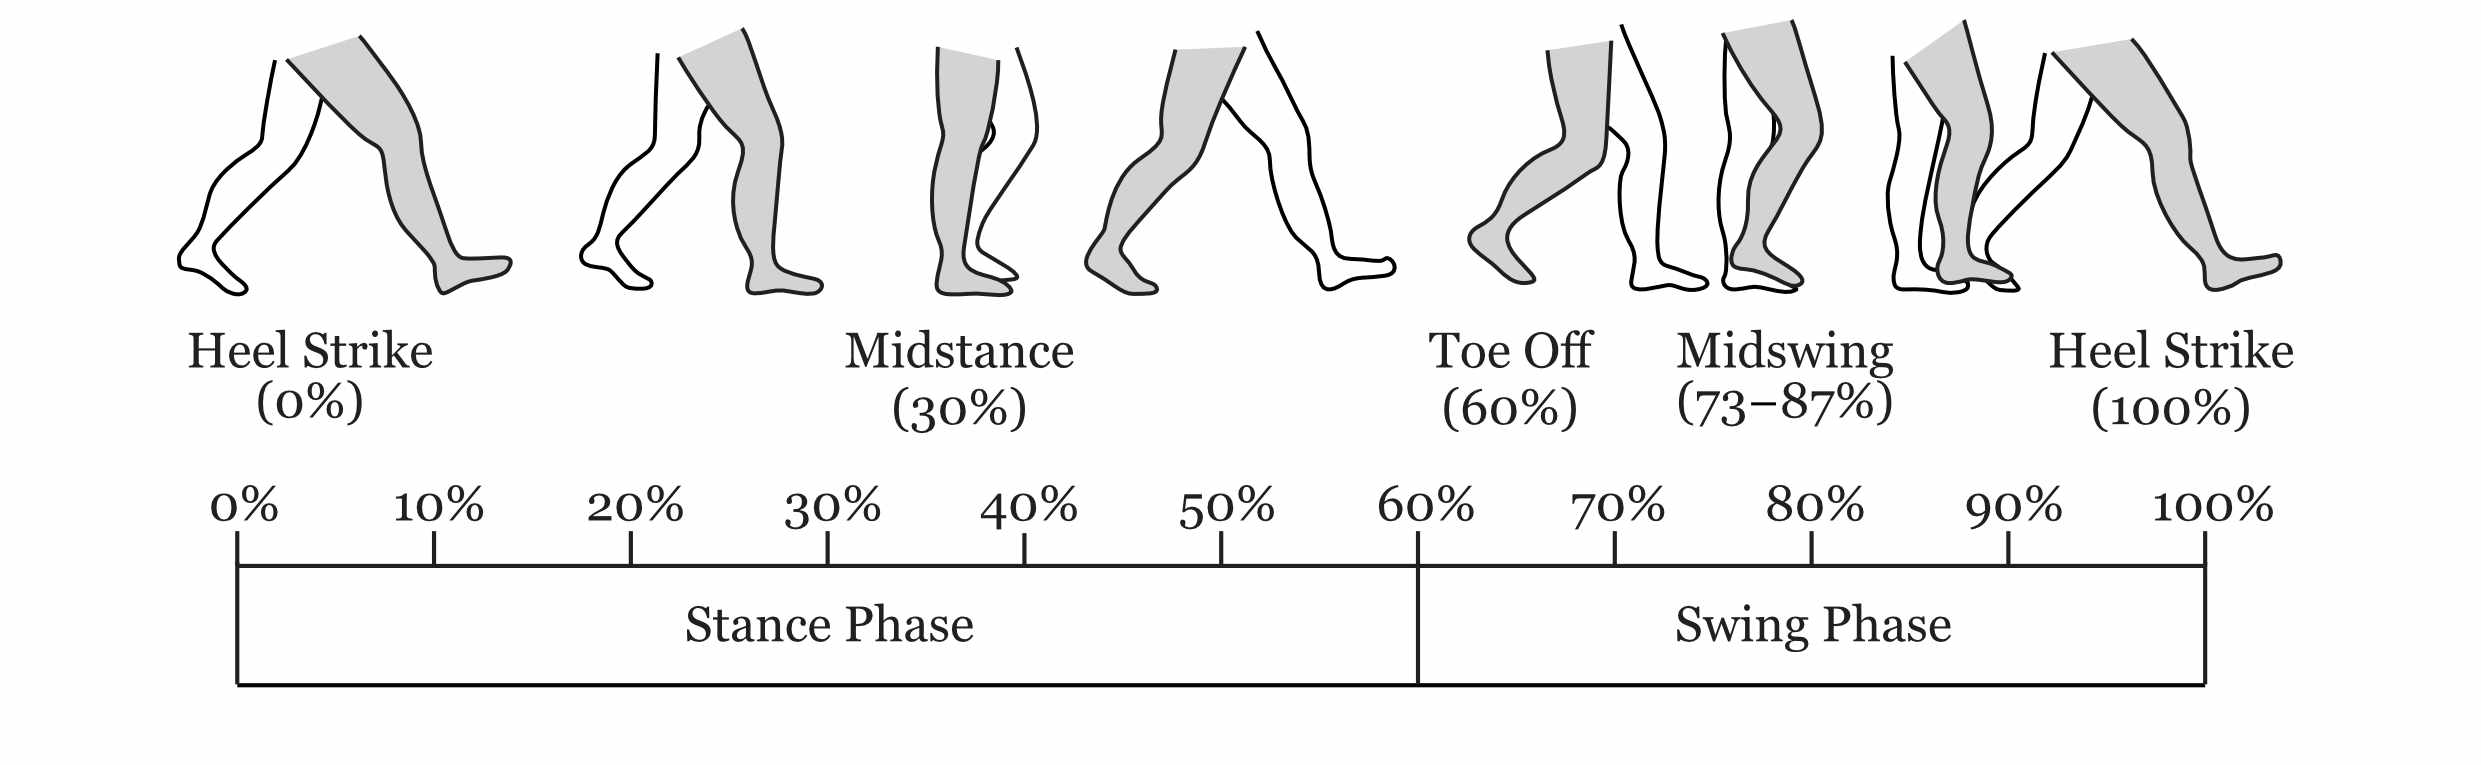
\includegraphics[width=\textwidth]{content/4-LSTM_Behaviour/Gait_Cycle.jpg}
    \caption{Human Gait Cycle during level walking. The~percentage timings of the gait events are approximate, they~vary depending on the individual and environment.}
    \label{fig:gait_cycle}
\end{figure}

It has been shown that gait events can be established from only extrema of the shank angular velocity in the sagittal plane (The sagittal plane divides the body into left and right, so~rotation in this plane is forward and backward motion of the shank) using a technique originally presented by Sabatini et al.~\cite{Sabatini2005}. IC/HS was found to line up with the minima following the peak swing velocity (PK) and TO was identified as the halfway point between the zero-crossing, negative to positive, and~the minima before peak swing. \mbox{Figure~\ref{fig:y-gyro-hs-to}} shows the gyroscope trace of a sensor attached to a subject's shank with the locations of the calculated TO and IC events indicated.

\begin{figure}[!hbt]
    \centering
    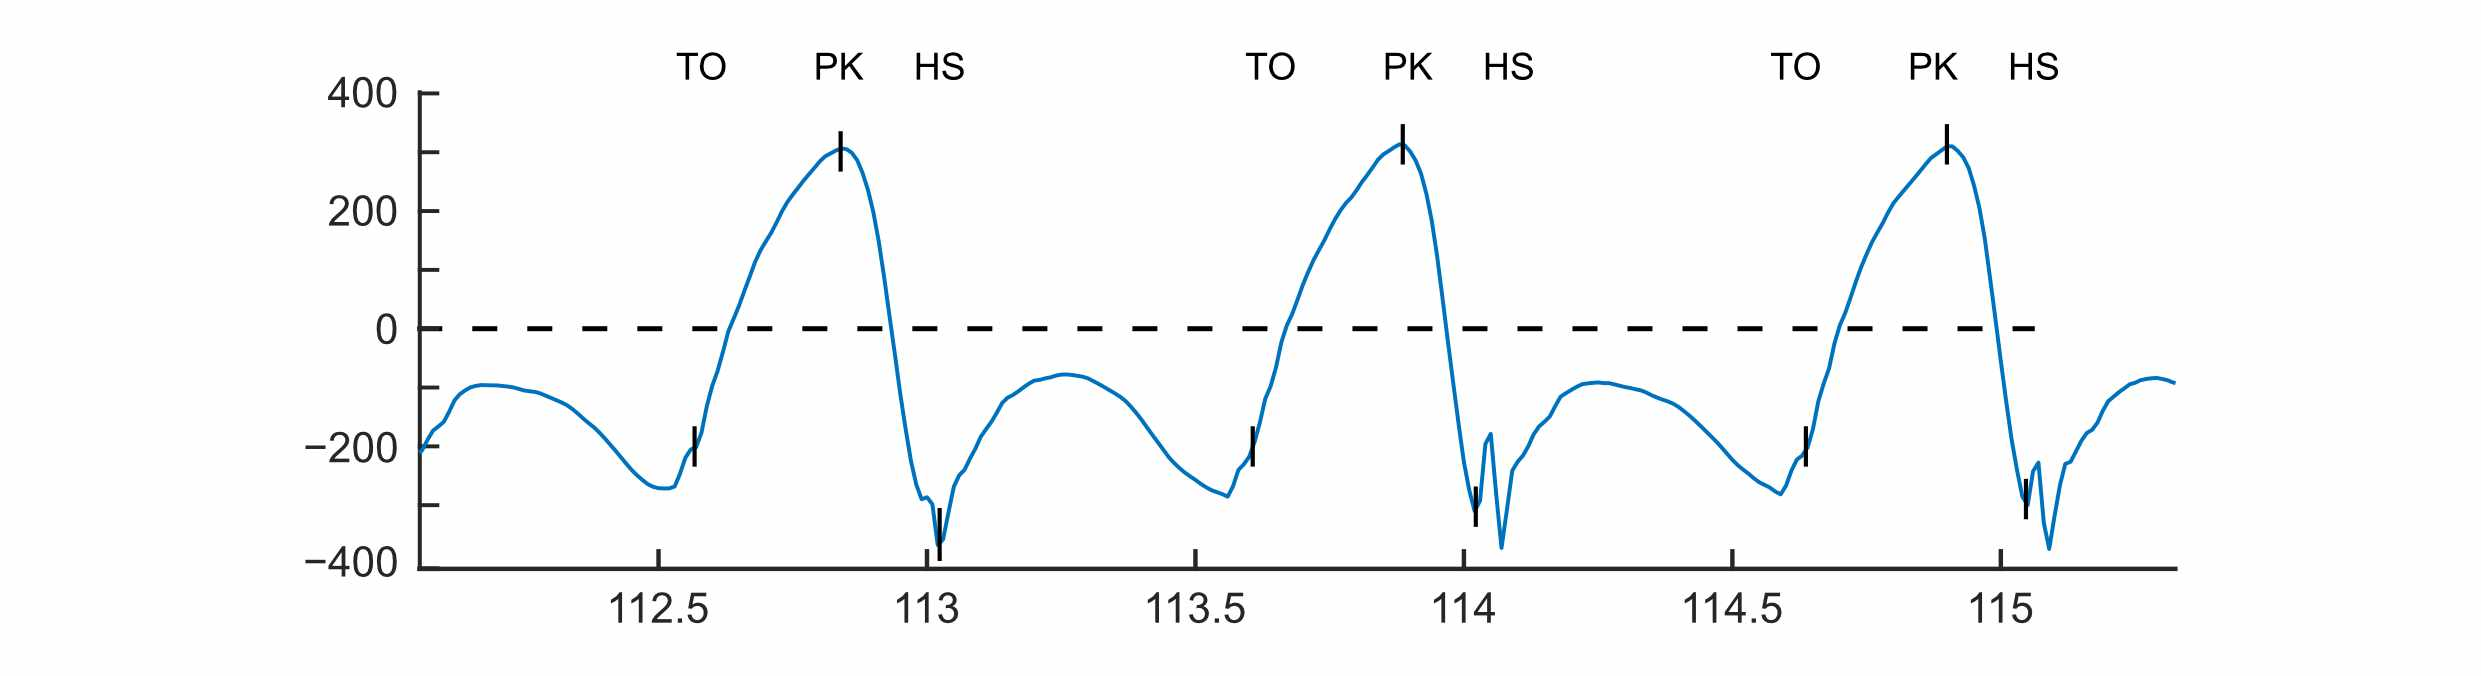
\includegraphics[width=\textwidth]{content/4-LSTM_Behaviour/gyro_trace_hs.jpg}
    \caption{Gait events extracted
 from the sagittal plane gyroscope signal. IC---Initial Contact, PK---Peak Swing, TO---Toe Off.}
    \label{fig:y-gyro-hs-to}
\end{figure}

% How does LMR relate to the human gait?
The action of the leg varies depending on the activity. To~accommodate this, powered prostheses will require multiple locomotive modes to achieve the different timing and power requirements. Therefore, automated recognition of the user's intentions and subsequent selection of the corresponding locomotive mode will be crucial to the performance of devices~\cite{Tucker2015, Windrich2016, Zhang2015}. In~order for amputees to have confidence in a prosthetic device, its~activity recognition must be timely, accurate and consistent and able to account for the individual gait characteristics~\cite{Pedroli2019, Sinha2011, Ponce2016}.

For the current generation of prosthetic devices, this~is achieved through hand-tuned heuristics. These methods identify and associate changing properties of sensor data with different activities. For~example, Coley et al. noted the variation in shank sagittal plane rotational velocity that occur when walking on stairs~\cite{Coley2005}. It~was found that during early stance there is an increase in rotational velocity during stair descent and a decrease during stair ascent when compared to level walking. The~current state of the art in LMR uses ML methods to accomplish activity recognition; these techniques will be discussed further in the next section.

%%%%%%%%%%%%%%%%%%%%%%%%%%%%%%%%%%%%%%%%%%%%%%%%%%%%%%%%%%%%%%%%%%%%%%%%
% Introduce ML in LMR and benefits over heuristics; RNN and LSTM theory; what have other people done in the area
\subsection{Long Short-Term Memory Networks}
\label{sec:lstm_therory}
LMR for active prostheses has conventionally been achieved through heuristic methods with handpicked features that are manually tuned for each individual ~\cite{Maqbool2017, Xu2018}. This approach is favored by the commercial market due to safety and regulatory concerns~\cite{Fluit2020}.  The tuning of these controllers is time-consuming and requires a highly skilled prosthetist. In the current state of the art for LMR techniques, the~focus has been on the use of ML techniques to automate the process of feature selection, output classification, and personalization~\cite{Labarriere2020}.

Many different machine-learning techniques have been investigated including, Support Vector Machines, Hidden Markov Models and Convolution Neural Networks (CNN) with success~\cite{Labarriere2020}. As sensor data from human gait is temporal, the best architecture for solving this will be one that can take into account the sequential nature of the input data. The Recurrent Neural Network (RNN) is an ML architecture suited to handling sequential data as it contains both vertical and horizontal connections. This means that cell activation is related to both the previous time step and the input. Information is therefore passed along the sequence as well as up through layers. Figure~\ref{fig:rnn_structure} shows the unfolded structure of a recurrent network. It can be seen that the activation of each cell is dependent on both its inputs and the hidden states of the previous time steps.

\begin{figure}[!hbt]
    \centering
    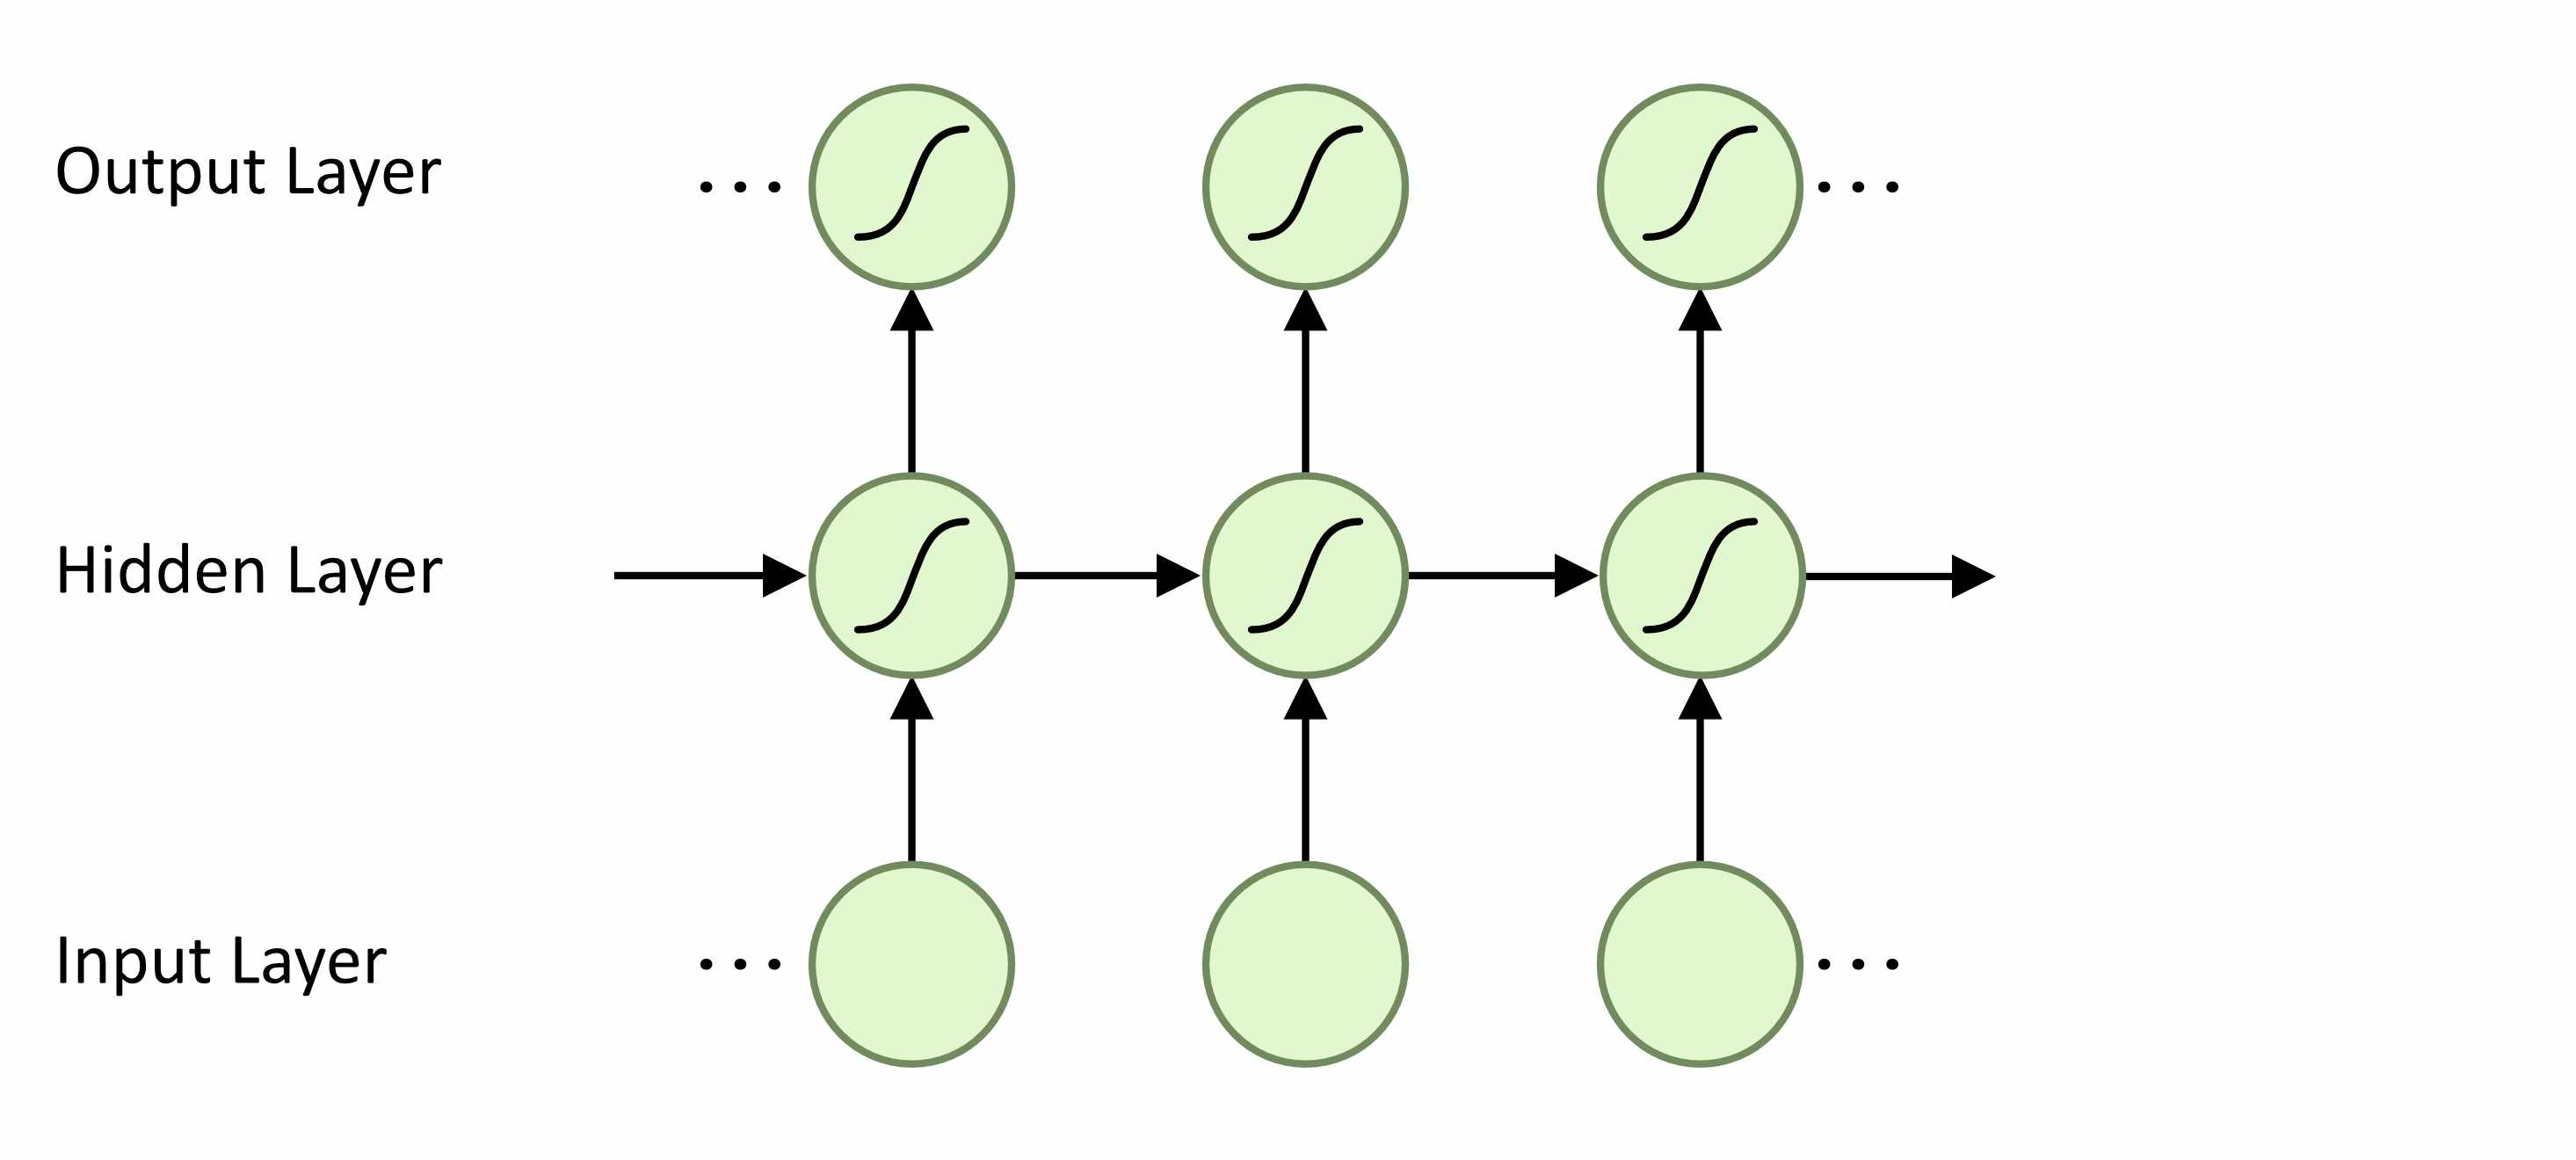
\includegraphics[width=0.7\textwidth]{content/4-LSTM_Behaviour/lstm/rnn_structure.jpg}
    \caption{Unfolded Recurrent Network.}
    \label{fig:rnn_structure}
\end{figure}

Each timestep in the network can contain several hidden states or units. This is represented by Equation (\ref{eqn:rnn_activation}) showing the activation input, $\mathbf{a}^t$. $\mathbf{a}$ is formed from the bias vector $\mathbf{b}$ plus the sum of input vectors $\mathbf{x}$ and previous hidden states $\mathbf{h}$, multiplied by the weight matrices $\mathbf{W}$ and $\mathbf{U}$ for hidden-to-hidden state and input-to-hidden state connections respectively~\cite{Goodfellow2015}. The shape of an RNN network is often described by its timesteps and units, for example, 128 $\times$ 6.

\begin{equation}
    \mathbf{a}^{(t)} = \mathbf{b} + \mathbf{Wh}^{(t-1)} + \mathbf{Ux}^{(t)}
    \label{eqn:rnn_activation}
\end{equation}

%What problems exist with them 
RNNs have been shown to produce good results in some sequential tasks, but~their application is limited by difficulty of training. The primary difficulty is the vanishing/exploding gradient problem. During gradient-based training methods, repeated multiplication by values that are not near one, along long dependency chains results in values that either vanish or explode. A vanishing gradient makes it challenging to know which direction the parameters should move to improve the cost function. Exploding gradients can make learning unstable. Non-gradient-based training has been tried, although to limited success~\cite{Graves2012, Goodfellow2015}.

% LSTM
The Long Short-Term Memory (LSTM) architecture solves the vanishing gradient problem by adding mechanisms for regulating information allowing it to be retained for long periods. Created by Hochreiter and Schmidhuber in 1997~\cite{Hochreiter1997} the LSTM is an RNN style architecture that includes gates to control information flow between cells, see~\mbox{Figure~\ref{fig:lstm_unit}.} Information flowing along the cell state can be modulated by the input and forget gate structures with the final output a filtered version of the cell state based on context from the inputs \cite{Olah2015}.

\begin{figure}[!hbt]
    \centering
    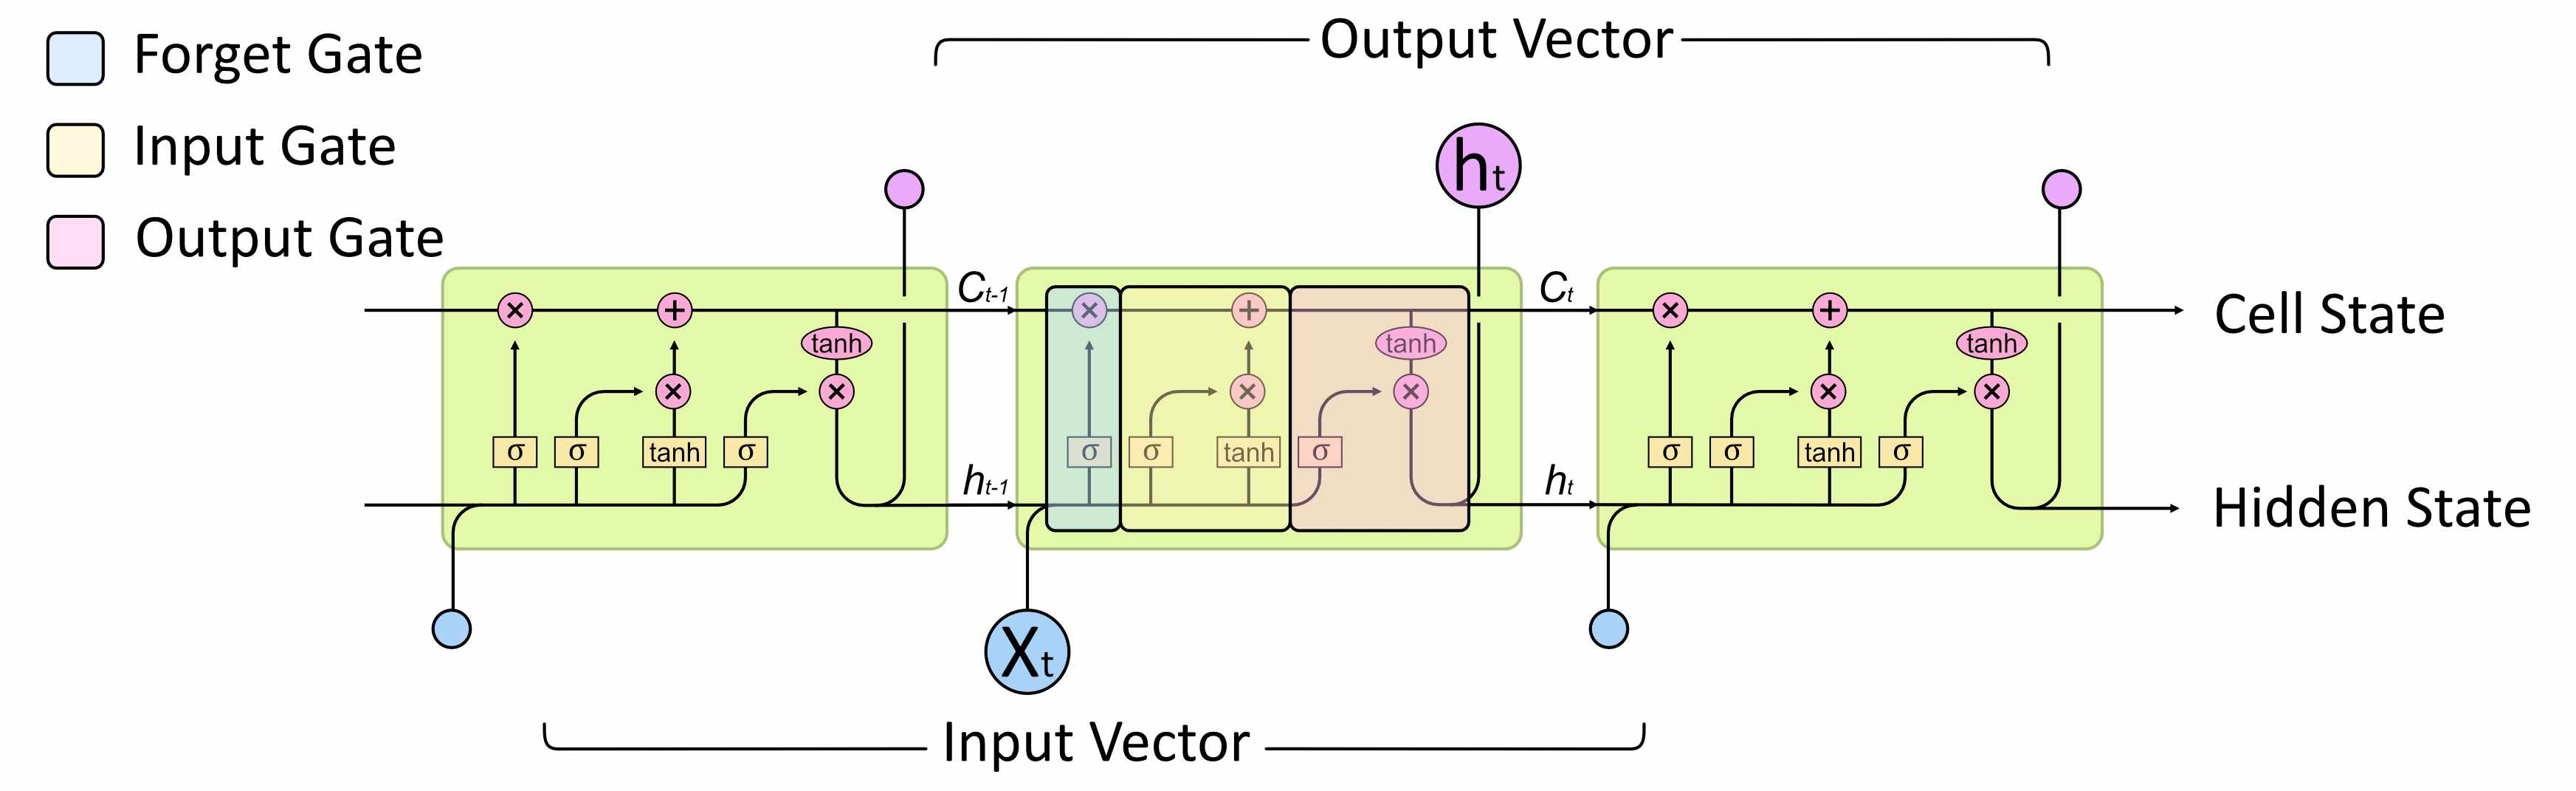
\includegraphics[width=0.9\textwidth]{content/4-LSTM_Behaviour/lstm/lstm_internal_operation.jpg}
    \caption{LSTM unit with input and output connections.}
    \label{fig:lstm_unit}
\end{figure}

\section{Related Works}
\label{sec:related_work}
In HAR tasks, LSTMs have been demonstrated to provide exceptional performance~\cite{Murad2017} although very little work has been done investigating this in the context of prostheses. Labarri\`ere et al. conducted a systematic review of the ML methods used in activity recognition; for assistive device LSTM networks were only used once~\cite{Labarriere2020}.

% Highly performing LSTM networks in LMR - Controlled conditions
LSTM networks have been found to perform highly in HAR and Activities of Daily Living (ADL) tasks. Murad and Pyun investigated Deep LSTM networks for LMR~\cite{Murad2017}. They~trained their network on common ADL datasets, presenting performance in comparison to other ML architectures on the same data sets. The~network they used took raw IMU data as its input, then interpreted the data using four LSTM layers before a late fusion dense layer and a SoftMax classifier were used to produce a class output. The number of units in the LSTM layers was not explicitly stated but appeared to be one. Performance is high achieving 96.7\% accuracy on the UCI-HAD dataset~\cite{Anguita2013} and an improvement on the presented previous classification attempts using CNN, SVM~and other networks. Tufek et al. replicated this result, achieving 93\% accuracy on the UCI-HAD data set using only a three-layer LSTM network~\cite{Tufek2020}.

However, the~accuracy presented is determined from the validation data, a~random 20\% of the source data, so~sufficient separation between training and validation data is not guaranteed. In~the compared work, a~mixture of evaluation techniques is used, most~commonly k-fold cross-validation techniques. With test data selected by leaving out participants~\cite{Koller2018, Sprager2015}. As such, it is not clear that a direct comparison can be made to demonstrate LSTM's superiority.

% Sensor fusion
Different sensor fusion approaches have been tried. Murad et al allowed a deep LSTM network to learn to fuse the sensor modalities~\cite{Murad2017}. Chung et al. used~an ensemble voting arrangement, where each channel modality of sensor data was passed through a separate LSTM network, with a weighted voting system forming the output classification~\cite{Chung2019}. This~achieved a slightly higher accuracy, of~94\%, than~using the sensors individually.

Multiple authors have developed models that use a series of CNN layer first to fuse sensor data from multiple modalities before passing it to a LSTM network~\cite{Abbaspour2020, Ihianle2020, Mutegeki2020, Wang2020, Mekruksavanich2020}. These achieve only minor improvements in performance classification with 95--96\% accuracies. Again, none of the authors were clear about the unit shape of their LSTM networks.

% LSTM network for assistive devices
There are few examples of LSTM networks being used in assistive devices. \mbox{Wang~et al. used~a Deep LSTM network to select locomotion modes for a lower extremity exo-skeleton~\cite{Wang2018}. Five~locomotion modes were classified (sitting, standing, walking and ascending/descending stairs) based on angular information from hip, knee~and ankle joints. A two-layer LSTM network with 128 timestep windows was used.} The hidden states of this were fed into a weighted mean before a SoftMax classifier. Again, the number of units per timestep was not specified. The classifier performed better than the other models tested achieving over 95\%.

% Use of non-amputee subjects as a substitute for amputees
Ben-Yue Su et al. presented work investigating intent prediction for trans-tibial amputees using IMU data and a CNN networks~\cite{Su2019}. Ten~non-amputee and one trans-tibial amputee were asked to perform short walks traversing a short staircase and ramp with a level surface either side. The~non-amputee subjects wore a hands-free crutch to simulate amputation. Three IMUs were attached to the thigh, shank and ankle of the ``healthy'' leg. The CNN classifier identified five steady states and eight transitions between states. An~accuracy of 94\% was achieved by the non-amputee subjects; this dropped to 89\% for the amputee for validation data. When~testing generalization to an unseen user, using Leave One Out Cross-Validation (LOOXV), this~dropped to 82\% for non-amputee subjects. Subject-specific training was recommended. Reasons for poor generalization were not investigated.

% Novel user performance
Research into the generalization of ML HAR Models to new users is limited. Dehghani et al. investigate the metrics used to evaluate the performance of classifiers, particularly regarding their performance on unseen data presented using k-fold cross-validation methods~\cite{Dehghani2019}. The~paper implements various forms of ML, such as Support Vector Machines (SVM) and Hidden Markov Models (HMM) but not LSTM. Dehghani found that using validation data to evaluate performance overestimates accuracy by 10--16\% as the validation data is too similar to the training data. Instead, individual subjects should be excluded and used as test subjects. The~reason for the worse generalization when presented with a novel user has not been investigated.

Investigations into LSTM networks for HAR/LMR have been primarily focused on achieving the highest possible classification accuracy. No~one has investigated the internal operation of the network, or~sensitivities to hyper-parameter selection for these applications. Dehghani et al. identified that model generalization to novel users is an area that also needs further investigation~\cite{Dehghani2019}. This~paper aims to address these areas.

\section{Materials and Methodology}
\label{sec:materials_and_methdology}
To complete the aims of this paper, a~dataset of human locomotion, methods for processing this data and a ML environment are required. This~section details the methodology used to provide this. It~is split into three sections, Sections \ref{sec:data_collection} and \ref{sec:pre-processing} detail the data collection and pre-processing, respectively. Section \ref{sec:machine_Learning} presents the ML environment and methods.

\subsection{Unsupervised Data Collection in Dynamic Natural Environments}
\label{sec:data_collection}
There are several commonly used data sets for LMR of non-amputees. The~OPPORTUNITY activity recognition dataset~\cite{roggan2010} contains 18  classes for Activities of Daily Living (ADL) such as opening/closing doors and drinking from a cup. Each~subject wore seven 6-axis IMUs and 12 3-axis accelerometers while they performed the prescribed actions. The~UCI-HAD dataset~\cite{Anguita2013} recorded subjects performing six activities: walking, stair ascent, stair descent, sitting, standing and lying while wearing a waist-mounted smartphone with onboard Magnetic, Angular Rate and Gravity (MARG) sensors. Both~of these data sets were recorded in controlled conditions, so~do not capture any variation in the activity that may occur due to the environment. Sztyler and Stuckenschmidt collected data from 15~subjects performing eight activities while wearing six wearable sensors. Recording took place in the same natural environments for each activity. Only~steady-state activities were captured and not the transition between them~\cite{Sztyler2017}. Due~to limitation in the identified data sets, a~new set of data is required. 

% Aim of data collection
The aim of the new data set was to record natural locomotion in an unstructured environment, capturing both steady-state and the transition between activities across different settings from a wide range of subjects. Collection of large quantities of data from amputees is very challenging, so~instead non-amputee subjects are used. Non-amputee subjects have a less varied gait than amputees, but~this can be countered by a larger population size.

% Sensor selection and location
Non-invasive wearable sensors, such~as Inertial Measurement Units (IMU), are~an appealing choice for developing such a system. IMUs~give fast update rates, 100s of Hz, are~non-invasive (small with minimal mounting constraints), low~cost and have reasonable accuracy. They~have been widely used in the field, all~of the latest generation of powered prosthetic knees investigated by Fluit et al contained IMUs~\cite{Fluit2020}.

% Which sensors did we use and why
The Suunto Movesense wearable IMU was used to collect activity data. This~is a COTS device containing a nine-axis MARG sensor and a Bluetooth Low Energy (BLE) radio in a small 10~g package. The~sensor housing contains a snap connector allowing it to be clipped on attachment hardware. A~variety of mounting hardware is available off the shelf. The~sensor is user-programmable allowing customized behavior through the Movesense API. To~enable the desired streaming application it was programmed to transmit compressed IMU data at 100Hz over its BLE connection to a custom app running on an android smartphone. The~devices come with Factory calibration for the IMU, no~additional IMU calibration was undertaken.

Five sensors were attached to each participant in the following locations: on the inside of both ankles using an elastic Velcro strap, on~each hip using a clothes/belt clip and across the chest using a heart rate strap. The~location of the sensors was selected to give wide coverage of body movements while providing easy, secure and non-invasive attachment to minimize discomfort and disruption to natural movement. Figure~\ref{fig:movesense_sensors} shows a subject wearing the five sensors.

\begin{figure}[!hbt]
    \centering
    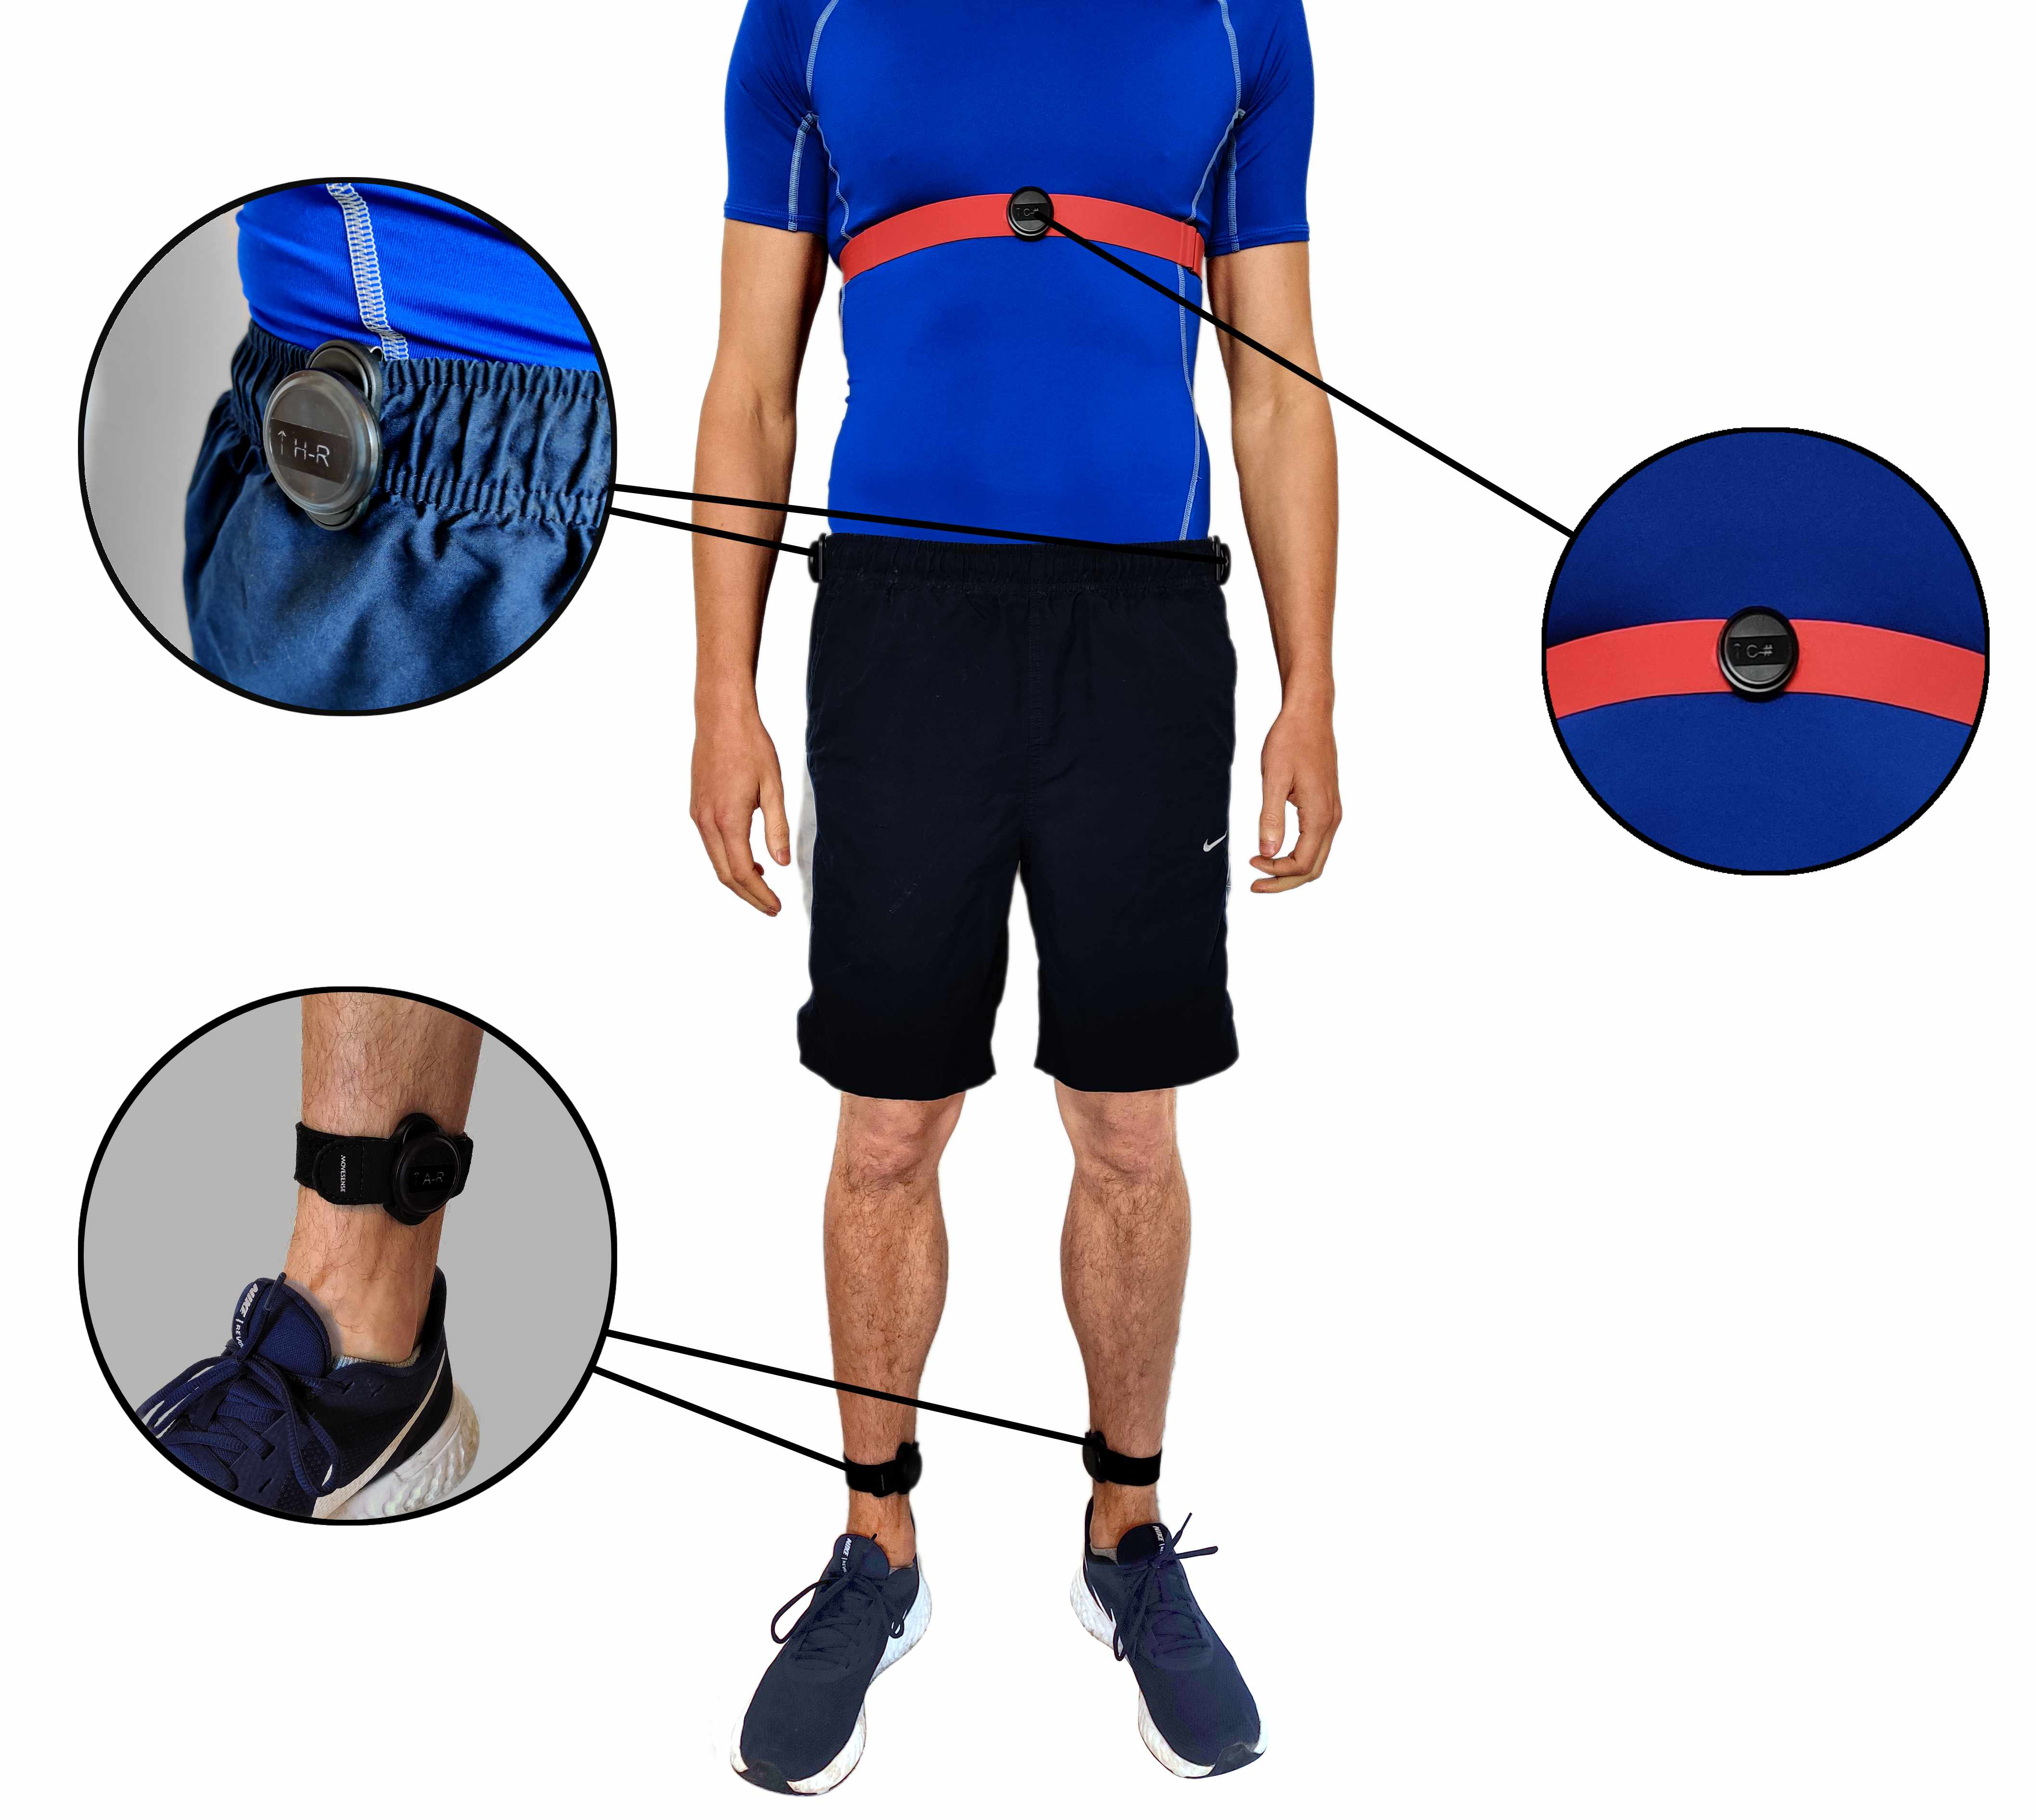
\includegraphics[height=220px]{content/4-LSTM_Behaviour/sensor_locations.jpg}
    \caption{Subject wearing the Movesense IMU sensors on both ankles, hips~and the chest.}
    \label{fig:movesense_sensors}
\end{figure}

To record data from the sensors, a~custom android app was created. This~formed a BLE connection to each device and saved the streamed data. During recording a series of buttons at the bottom of the screen could be used for real-time labelling of activities. Once~recording had finished the subject was presented with an upload screen allowing metadata to be added. The~file could then be shared anonymously with the researchers using Google's Firebase cloud services. A~screenshot of the app in recording mode is shown in Figure~\ref{fig:data_collection_diagrams}.

\begin{figure}[!hbt]
    \centering
    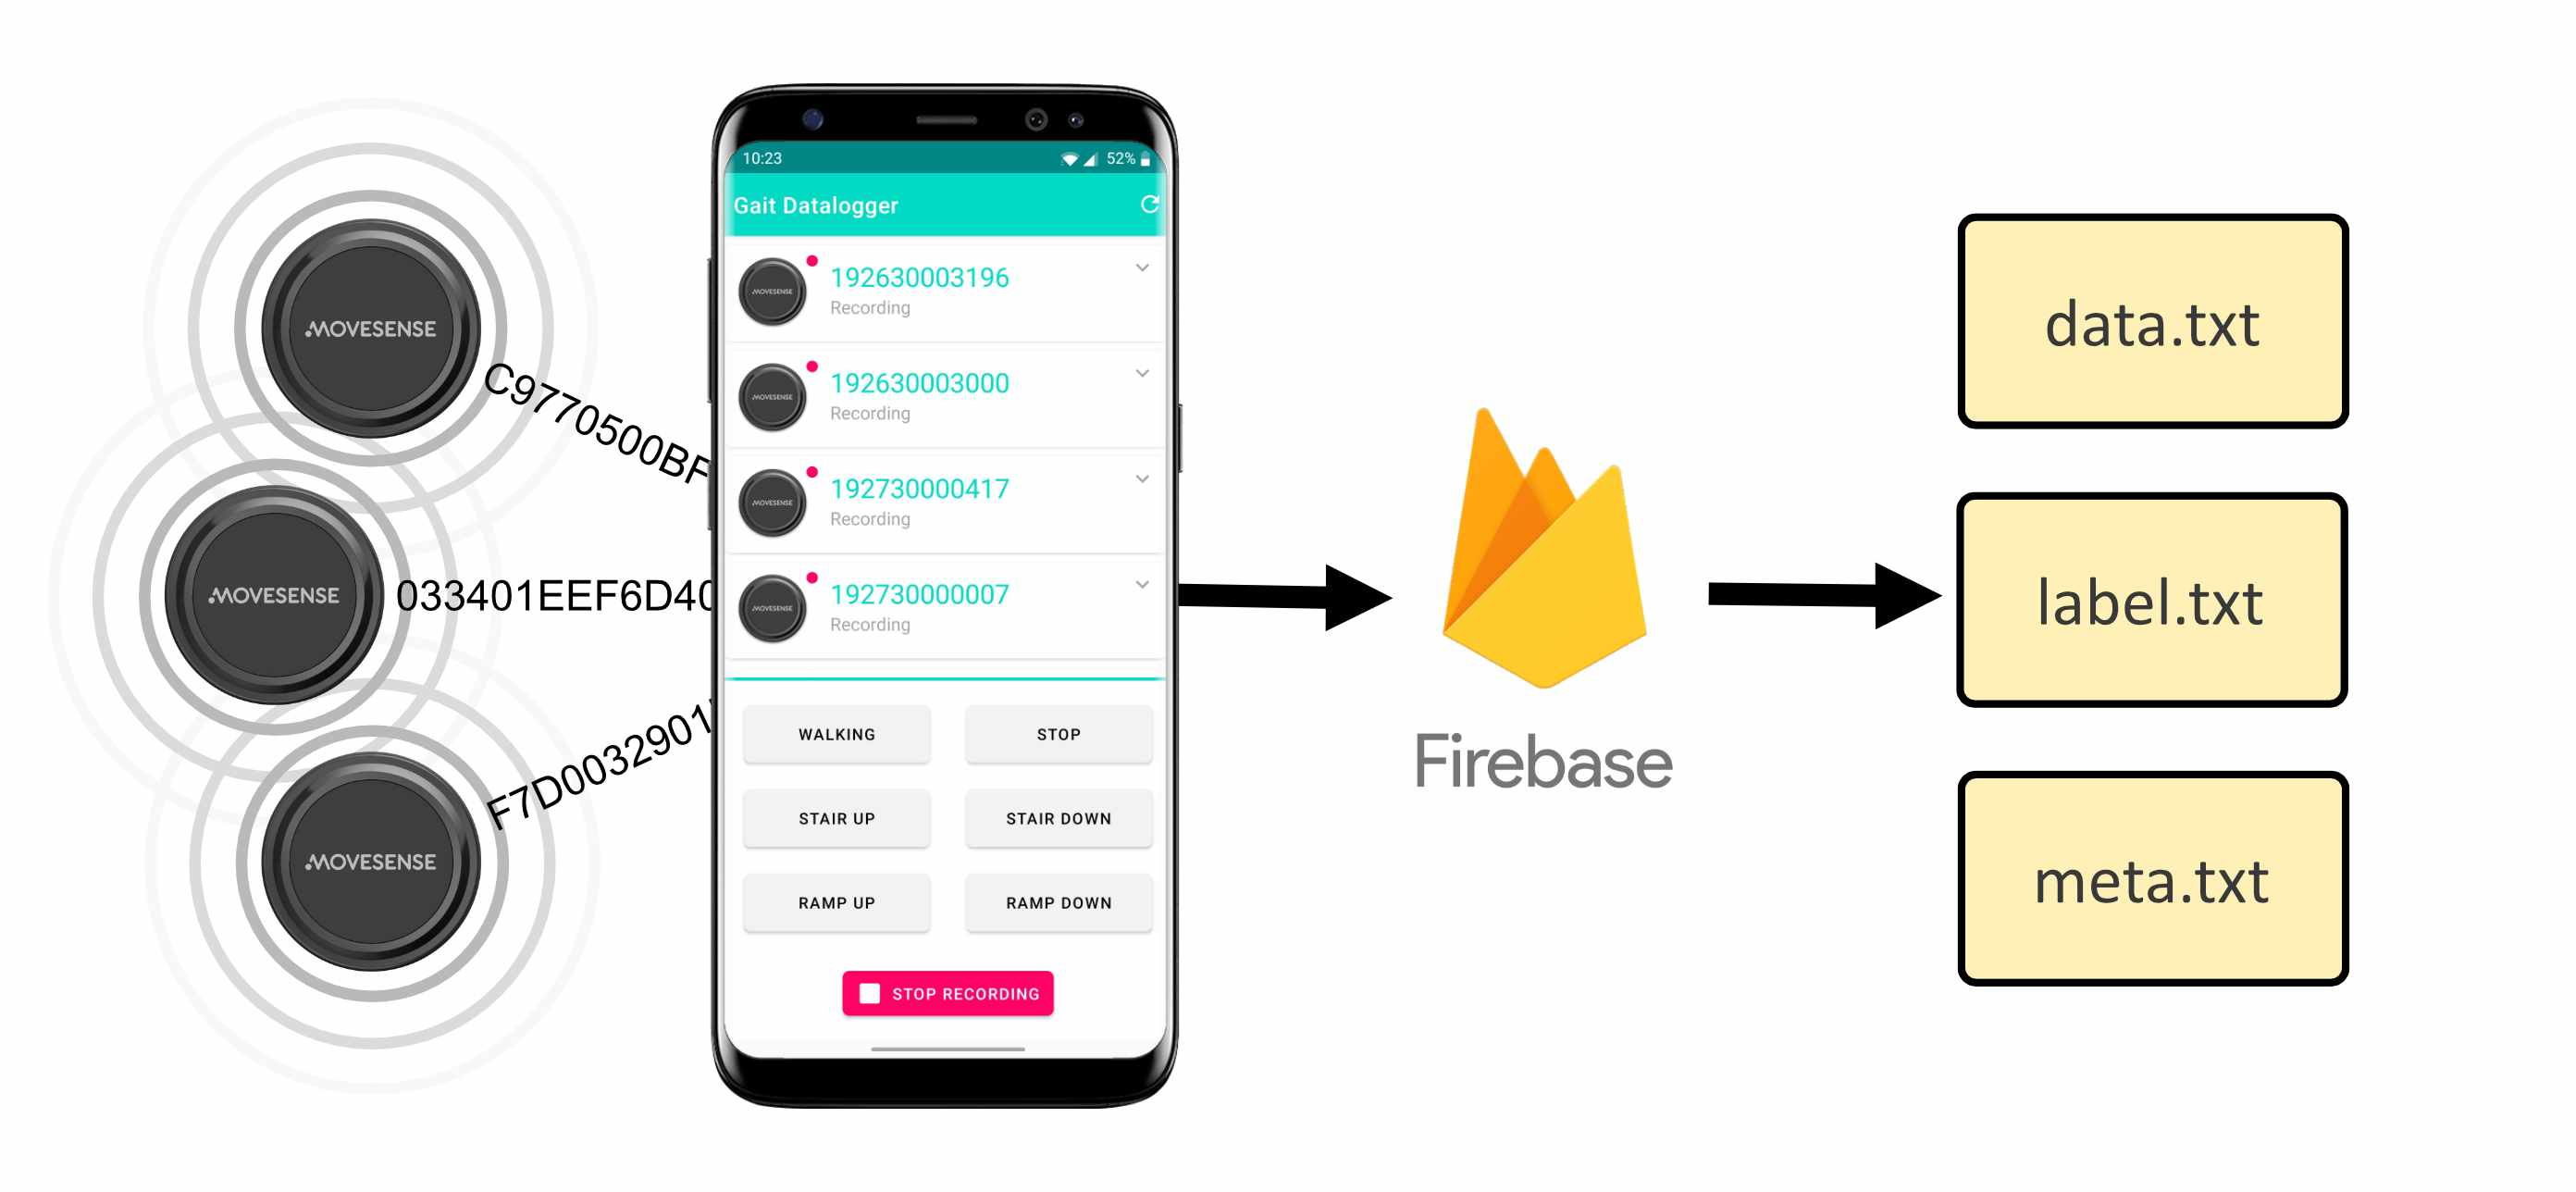
\includegraphics[width=0.8\textwidth]{content/4-LSTM_Behaviour/sensor_collection.jpg}
    \caption{Custom Android app with connected sensors and illustration of Firebase upload system.}
    \label{fig:data_collection_diagrams}
\end{figure}

Study subjects were provided with instructions on how to use the sensing equipment, and~the activity classes, then~allowed to record as they wished. The~following activities were selected, Walking (W), Stair Ascent (SA), Stair Descent (SD), Ramp~Ascent (RA), Ramp~Descent (RD) and Stopped (S). Labarri\`ere et al. identified these as the most commonly investigated and they require no equipment or skill to perform~\cite{Labarriere2020}. The~study received ethical approval from the University of Bath Research Ethics Approval Committee for Health (REACH), reference \textit{EP 19/20 003}.

% Participant instructions
Twenty-two participants of a wide variety of age (mean 29, std~10), gender (17M, 5F), and~physique were chosen to give a broad data set. Participants were instructed to walk around a varied environment with the sensor on while labelling the six activity classes. No~further instructions on how the recording should be conducted were provided. A~total of 268~min  of data was collected, which includes 1170~transitions between activities. Table \ref{tab:data_collected_summary} contains a summary of the data collected. The~number of steps was produced by summing the peak swing gait events for each label.

% % Dataset Statistics
% \begin{specialtable}[H]
%     \centering
%     \caption{Quantity of data collected for each activity.}
%     \label{tab:data_collected_summary}
%     \setlength{\cellWidtha}{\columnwidth/4-2\tabcolsep+0.0in}
% \setlength{\cellWidthb}{\columnwidth/4-2\tabcolsep+0.0in}
% \setlength{\cellWidthc}{\columnwidth/4-2\tabcolsep-0.0in}
% \setlength{\cellWidthd}{\columnwidth/4-2\tabcolsep-0.0in}
% %\setlength{\cellWidthe}{\columnwidth/8-2\tabcolsep-0.0in}
% %\setlength{\cellWidthf}{\columnwidth/8-2\tabcolsep-0.0in}
% %\setlength{\cellWidthg}{\columnwidth/8-2\tabcolsep-0in}
% %\setlength{\cellWidthh}{\columnwidth/8-2\tabcolsep-0in}%
% \scalebox{1}[1]{\begin{tabularx}{\columnwidth}{>{\PreserveBackslash\centering}m{\cellWidtha}>{\PreserveBackslash\centering}m{\cellWidthb}>{\PreserveBackslash\centering}m{\cellWidthc}>{\PreserveBackslash\centering}m{\cellWidthd}}
% \toprule
%         \textbf{Activity} & \textbf{Samples} & \textbf{Time (min)} & \textbf{Number of Steps} \\
%          \midrule
%          Walking & 1,075,211 & 179 & 9438 \\
%          Stair Ascent & 139,922 & 23 & 1286 \\
%          Stair Descent & 122,379 & 20 & 1280 \\ 
%          Ramp Ascent & 73,328 & 12 & 656 \\
%          Ramp Descent & 79,436 & 13 & 754 \\
%          Stop & 121,027 & 20 & - \\
%          \midrule
%          \textbf{Total} & 1,611,303 & 268 & 13,414\\
%           \bottomrule
% \end{tabularx}}
% \end{specialtable}
\begin{table}[!hbt]
    \centering
    \caption{Quantity of data collected for each activity.}
    \label{tab:data_collected_summary}
    \begin{tabularx}{\textwidth}{YYYY}
        \textbf{Activity} & \textbf{Samples} & \textbf{Time (min)} & \textbf{Number of Steps} \\
        \hline
        Walking & 1075211 & 179 & 9438 \\
        Stair Ascent & 139922 & 23 & 1286 \\
        Stair Descent & 122379 & 20 & 1280 \\ 
        Ramp Ascent & 73328 & 12 & 656 \\
        Ramp Descent & 79436 & 13 & 754 \\
        Stop & 121027 & 20 & - \\
        \hline
        \textbf{Total} & 1611303 & 268 & 13414
    \end{tabularx}
\end{table}
\clearpage


% \setcounter{page}{\numexpr\x + 23\relax}

\section{Post-commentary}
Since being published, nine papers have cited the article\footnote{as of the 27\textsuperscript{th} January 2022}. A number of these citations have used the paper as an example use case for an \acrshort{lstm} network\cite{Uddin2021, Du2021, Velezguerrero2021, Low2022, Bittibssi2022} and data capture methods\cite{Shin2021, Su2021}.
%\cite{Hamayel2021, Priya2021} Just used as reference for how an LSTM works - weirdly

% What was the big takeaway from this paper - demonstrates the need for personalisation
The paper's outcomes expressed the need for model personalisation to achieve acceptable performance for novel users. It also noted the need for additional testing to demonstrate the suitability of these techniques for amputees. These needs will be explored further in the subsequent chapters.

\chapter{Model Personalisation}
\label{chp:personalisation}
The previous chapter investigated classification accuracy for a general or subject agnostic \acrshort{lstm} based \acrshort{lmr} model. Due to the variability between individuals classification accuracies of greater than 80\% could not be achieved for unseen novel subjects. Instead a form of personalisation is necessary to adapt the model for novel subjects. Within this chapter methods for achieving this will be explored. Before attempting to produce a model for amputees methods will be developed and tested on non-amputees.

The collection of labelled data for an individual is burdensome therefore any system that can be used to reduce the labelling requirements is advantageous. Transfer learning approaches allow large training sets pooled from many individuals to be leveraged to reduce target data requirements on the assumption they hold relevant information.\cite{Fallahzadeh2017, Schneider2021}

From this point forward the following naming convention will be used; the subject of personalisation will be referred to as the target and all other subjects will be referred to as source.

Within this chapter we will investigate whether a large population of source data can be used to improve the performance and efficiency of producing a personalised \acrshort{lstm} \acrshort{lmr} classifier for a target individual.

The contributions of this Chapter are as follows:
\begin{itemize}
    \item A method for evaluating personalisation \acrshort{lmr} models from a set of real world continuous gait data
    \item Demonstration of the impact on classification performance of increased target training data
\end{itemize}

The Chapter is presented as follows. First, in Section \ref{sec:personalisation-related-works}, related literature is presented. This is followed by the methods and materials used in the study in Section \ref{sec:personalistaion-methods}. The results of a baseline model trained from only target data are presented in Section \ref{sec:personalisation-baseline-model-results}, followed by the results and analysis for penalisation techniques in Section \ref{sec:model-personalisation-results}. Finally discussion and conclusions are presented in Sections \ref{sec:personalisation-discussion} and \ref{sec:personalisation-conclusions} respectively.

%------------------------------------------
\section{Related Works} % Does this need more detail to back up the research gaps identified
\label{sec:personalisation-related-works}
\acrshort{ml} classifiers are constructed with the assumption that the probabilistic distribution between the source and target domain are equal\cite{Farahani2020}. In reality this is never the case and as such methods to account for differences between domains have been developed. Where this is adaptation between humans this is typically termed personalisation.

Personalising of \acrshort{ml} models is a common issue and has been addressed in many different ways across different areas of research\cite{Mairittha2021, Tomanek2021}. Schneider et al divides personalisation methods into two groups, shaping and data grouping\cite{Schneider2021}. In shaping the behaviour of a network is biased or shaped towards an individual, in data grouping the target data set is enlarged by adding data from similar individuals to it. Both of these techniques take advantage of data from others to reduce labelled data requirements for the target subject\cite{Shor2020}. The following survey of literature will be divided by these two categories. 

Shaping the behaviour of a network can occur at different times during training. Two are common, the beginning, early, or the end, late. In early shaping the model is first trained with target data followed by a larger set of source data. The opposite is done in late shaping, where a general model formed from a large source training set is fine-tuned with target data. By updating a trained model using data from a different distribution, the knowledge from an existing model can be transferred. This method is common and normally referred to as transfer learning.\cite{Schneider2021}

Transfer learning is the ability to extend what has been learnt in one context to another nonidentical but similar context\cite{Fallahzadeh2017}. The change in context can be either the task, the domain or both. Transfer learning is appealing, since it is often faster, as a model does not need to be trained from scratch for each target. 

Transfer learning is generally achieved in two phases. First a generic global model is trained from a set of source data. Then it is adapted to the target by additional training using only the targets data. The influence of the target is controllable by both the number of iterations and number of layers trained.\cite{Schneider2021, Mireshghallah2021}

A subset of transfer learning is domain adaptation where the domain changes but the task remains the same\cite{Goodfellow2015}. Domain adaptation techniques often focus on learning and apply a mapping between the source and target input data rather than fine-tuning an existing model.

%-----------------------------
% Shaping/Transfer learning
Yoon et al presented a transfer learning scheme for personalisation of a \acrshort{lstm} based language model for generating stylised sentence completion. Their work focuses on techniques that allow transfer learning using only a small amount of target data and limited computing resource. To achieve this two schemes are investigated - inserting and training a surplus layer between the output and last LSTM layer; and freezing the first n-layer and fine-tuning just the subsequent layers. Both methods reduce the training requirements when compared to fine-tuning the entire base model while achieving similar performance.\cite{Yoon2017}

Fu et al developed a domain adaptation method for unlabelled target data denoted Joint Probability Domain Adaptation with Improved Pseudo Labels (IPL-JPDA). The method produces a transformation matrix to adapt the input data of the target to the source domain removing the need to adjust the model itself. The study collects labelled data for a set of ten subjects in a controlled environment. This data is then split into target and source data sets with the performance tested using a cross validation method. Personalisation is undertaken using the IPL-JPDA method and tested against a subset of the data windows for each activity. Their method achieves an accuracy of $93.2\%$ accuracy, an increase of around $2\%$ over the baseline.\cite{Fu2021}


%-----------------------------
% Data grouping - Training from similar users
The other category of personalisation is data grouping. In data grouping the target data set is enlarged by supplementing it with data from existing source data. Each individual will differ from each other, but it should be expected that the population as a whole or a subset of it are similar\cite{Schneider2021, Nguyen2021}. Identifying and combining similar individuals is the main area of concentration for this field.

Ferrari et al investigated data grouping personalisation methods that weight the influence of training data based on similarity to the target subject. Similarity was evaluated through physical traits (age, weight and height) and on comparison of the input feature vector. Three publicly available \acrshort{adl} data sets were used to test performance, niMiB-SHAR\cite{Micucci2017}, Mobiact\cite{Vavoulas2016} and Motion Sense\cite{Katevas2014}. All data was collected in controlled conditions. An Adaboost classifier was trained for each target subject using the weighted training data. The experiment was repeated with and without target data included in the training set. Excluding the target saw only a small improvement in performance, compared to without similarity biasing. Including the target in the training data increased classification accuracy by $>10\%$, on average achieving $87.39\%$. This suggests weighting the training data set towards the target subject has a larger influence on performance than similarity.

Nguyen et al presented another data grouping technique using a DeepConvLSTM architecture. The model used learnt features, so determining the similarity of the feature vector was not possible. Instead the output of the last LSTM layer was used as a pseudo for the feature vector. A \acrfull{fid} algorithm was used to score the similarity of subjects. The score was then used to group source subjects, by selecting the closest $n$ neighbours and also clustering subjects into communities. It was noted this correlated closely with the physical characteristics. The groups were then used to both train a new model from scratch and fine-tune a general model. Fine-tuning a global model proved more effective. This method improved the global model performance by $3.5\%$ to $84.2\%$. The experiments were performed on four public data sets; OPPORTUNITY\cite{Roggen2009}, Daphnet Gait\cite{Sigcha2020}, Wetlab\cite{Scholl2015} and Mobiact\cite{Vavoulas2016} data sets, all of which were collected in closed controlled environments.\cite{Nguyen2021}


%-----------------------------
% Combination - retrain general model based on similar users
Several authors attempted to combine both transfer learning and data grouping techniques. These methods used data grouping techniques to produce a base model which was subsequently fine-tuned using data from the target.

Wang et al presents a source selection and transfer learning approach for a \acrshort{cnn}-\acrshort{lstm} architecture for unsupervised transfer learning. First source subjects were selected based on a closeness score. This score was a combination of a cosine similarity function and a hand selected value based on physical similarity between sensor locations. Using the selected source subjects a \acrshort{ml} model was trained. Fine-tuning of the model was achieved by inserting and training an adaption layer between the last two dense layers. The investigation was performed using the OPPORTUNITY\cite{Roggen2009}, PAMAP2\cite{Reiss2012} and UCI DSADS\cite{Altun2010} data sets which again were all collected in controlled conditions.\cite{Wang2018a}

Cruciani et al presents work on personalising an activity recognition model built from the subset of a general population. The subset of subjects was selected by comparing the similarity of manually selected features. Those with the closest matching traits were used to generate the base model. Further training was then performed using a small amount of target  data. This approach achieved a ~5\% improvement in performance when compared to selecting a source subset at random\cite{Cruciani2020}. The experiment was performed on the \acrshort{adl} Extrasensory data set published by Vaizman et al\cite{Vaizman2017}, this data set was collected using a smartphone in uncontrolled conditions with limited guidance given on how to collect or label the data.

From the literature surveyed the following gaps were identified:
\begin{itemize}
\item No methods for effectively testing the general performance of a transfer learning system from continuous real world environments
\item No comparison between the performance that could be achieved by just training a model with the target subject's data
\item There has been limited work on understanding how performance improves with increasing amounts of target data
\item None have investigated the use of IMU ankle data
\end{itemize}


%------------------------------------------
\section{Methods and Materials}
\label{sec:personalistaion-methods}
%Introduction to section
Within this section, the methods and materials required to address the research question will be detailed. The section is structured as follows: first, details of an expanded data set of labelled real world HAR data are provided; then, new methods for dividing this data into representative data sets are developed; finally, \acrshort{ml} personalisation methods are presented.

% Data collection
\subsection{Gait Data}
For these experiments a HAR data set, which contains both a large population and a large quantity of data for a small subset, is required. Data for a large number of subjects has previously been collected. Therefore only additional data for the subset of target subjects is required. These will be Subjects 1, 3 and 9. The additional data was collected in the same manner as before, described in Section \ref{sec:methods-data-collection}.

Only data from the shank mounted accelerometer and gyroscope will be used. As from previous work, in Chapter \ref{chp:lstm-general}, minimal performance improvement was seen for the additional sensors. 

%------------------
% Data augmentation (Combining left and right ankle data)
To reduce the data required for the target subject, data for both the left and right ankle was combined. The transformation in Equation \ref{eqn:left-right-transformation} was used to rotate and reflect the left ankle to match the right ankle. In Equation \ref{eqn:left-right-transformation} $V$ is the original data and $V_t$ is the transformed data. 

Figure \ref{fig:personalistaion_target_subjects_gyro_trends} shows the mean signals from the shank mounted gyroscope in the saggital plane for each of the target subjects. Note data is not normalised. Only stair descent for subject 3 shows any obvious differences between left and right ankles. Therefore it is reasonable to combined ankle data in this way.

\begin{equation}
    V_t = \begin{bmatrix}
    1 & 0 & 0 \\
    0 & -1 & 0 \\
    0 & 0 & -1
    \end{bmatrix} V
\label{eqn:left-right-transformation}
\end{equation}

\begin{figure}[p]
    \begin{tabular}{lccc}
        & \textbf{Subject 1} & \textbf{Subject 3} & \textbf{Subject 9} \vspace{0.2cm}\\
        \rotatebox{90}{\enspace\qquad \textbf{Walking}} &
        \begin{subfigure}[b]{0.275\textwidth}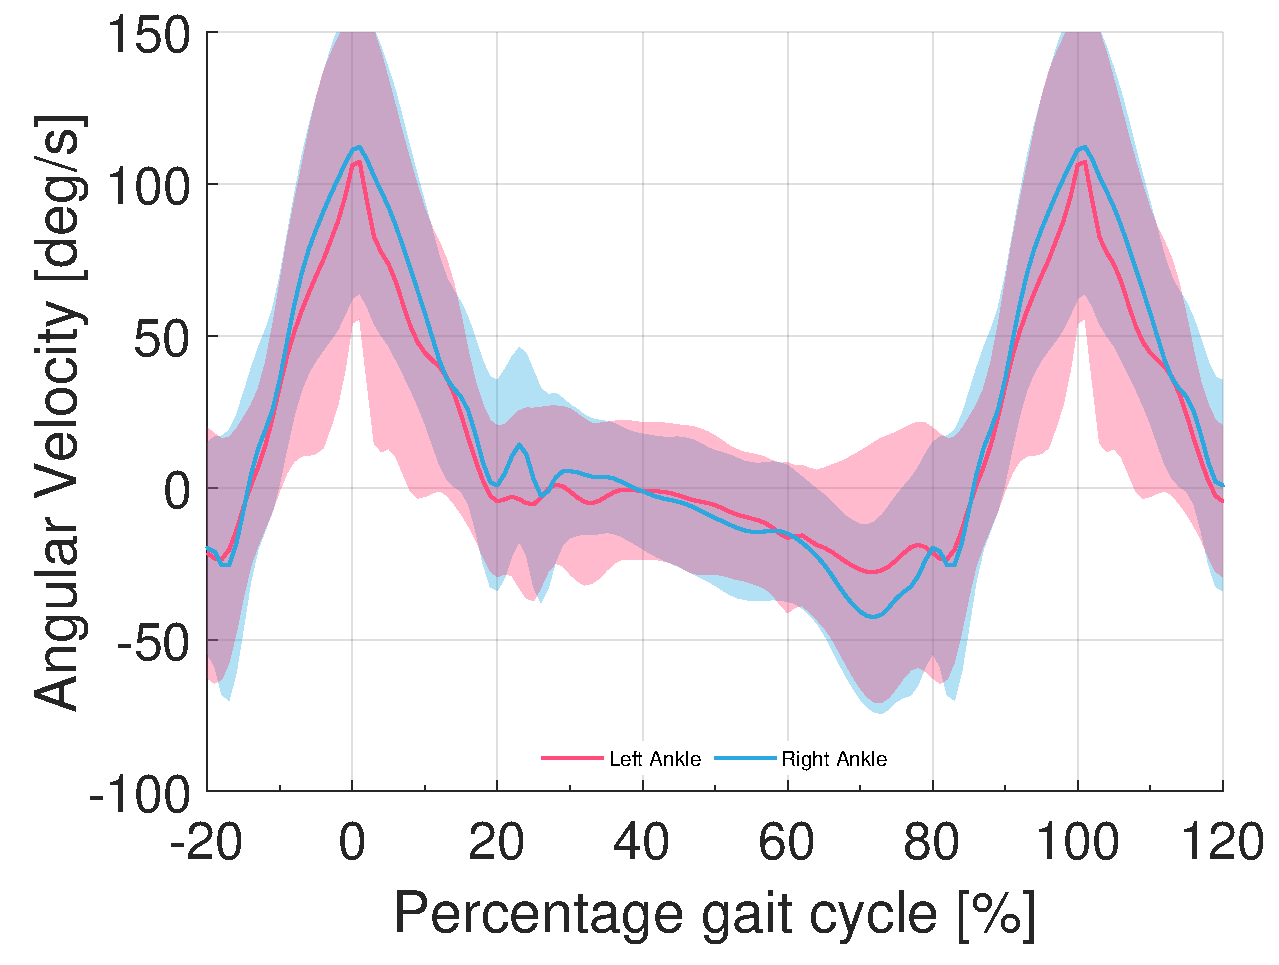
\includegraphics[width=\linewidth]{content/5-Personalisation/Gyro_Trends_For_Targets/ch5_gait_trends_subject_01_activity_walking.pdf}\end{subfigure} & \begin{subfigure}[b]{0.275\textwidth}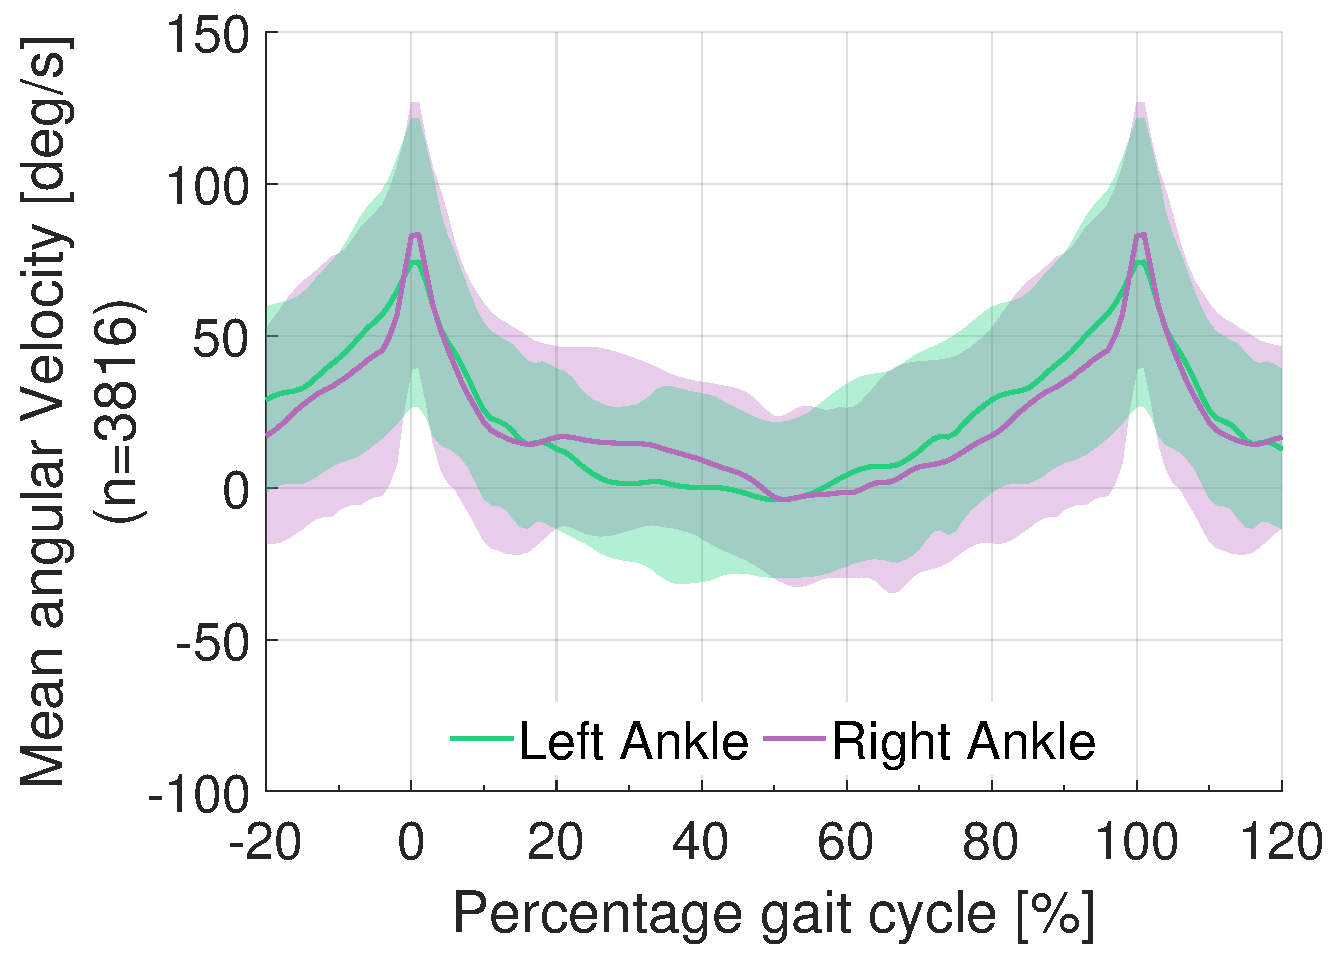
\includegraphics[width=\linewidth]{content/5-Personalisation/Gyro_Trends_For_Targets/ch5_gait_trends_subject_03_activity_walking.pdf}\end{subfigure} &
        \begin{subfigure}[b]{0.275\textwidth}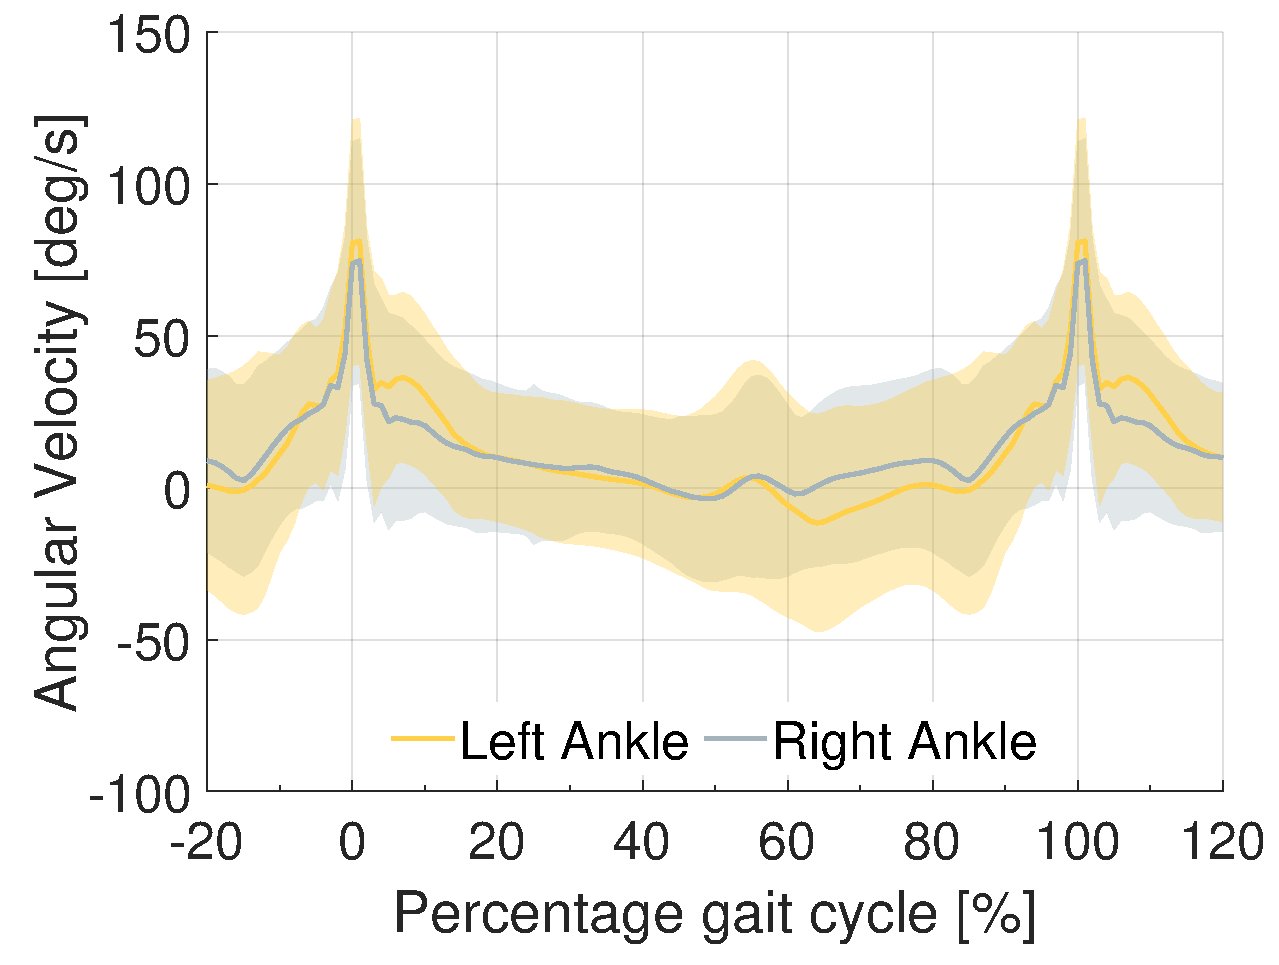
\includegraphics[width=\linewidth]{content/5-Personalisation/Gyro_Trends_For_Targets/ch5_gait_trends_subject_09_activity_walking.pdf}\end{subfigure} \\
        \rotatebox{90}{~\quad \textbf{\glsentrylong{ra}}} & 
        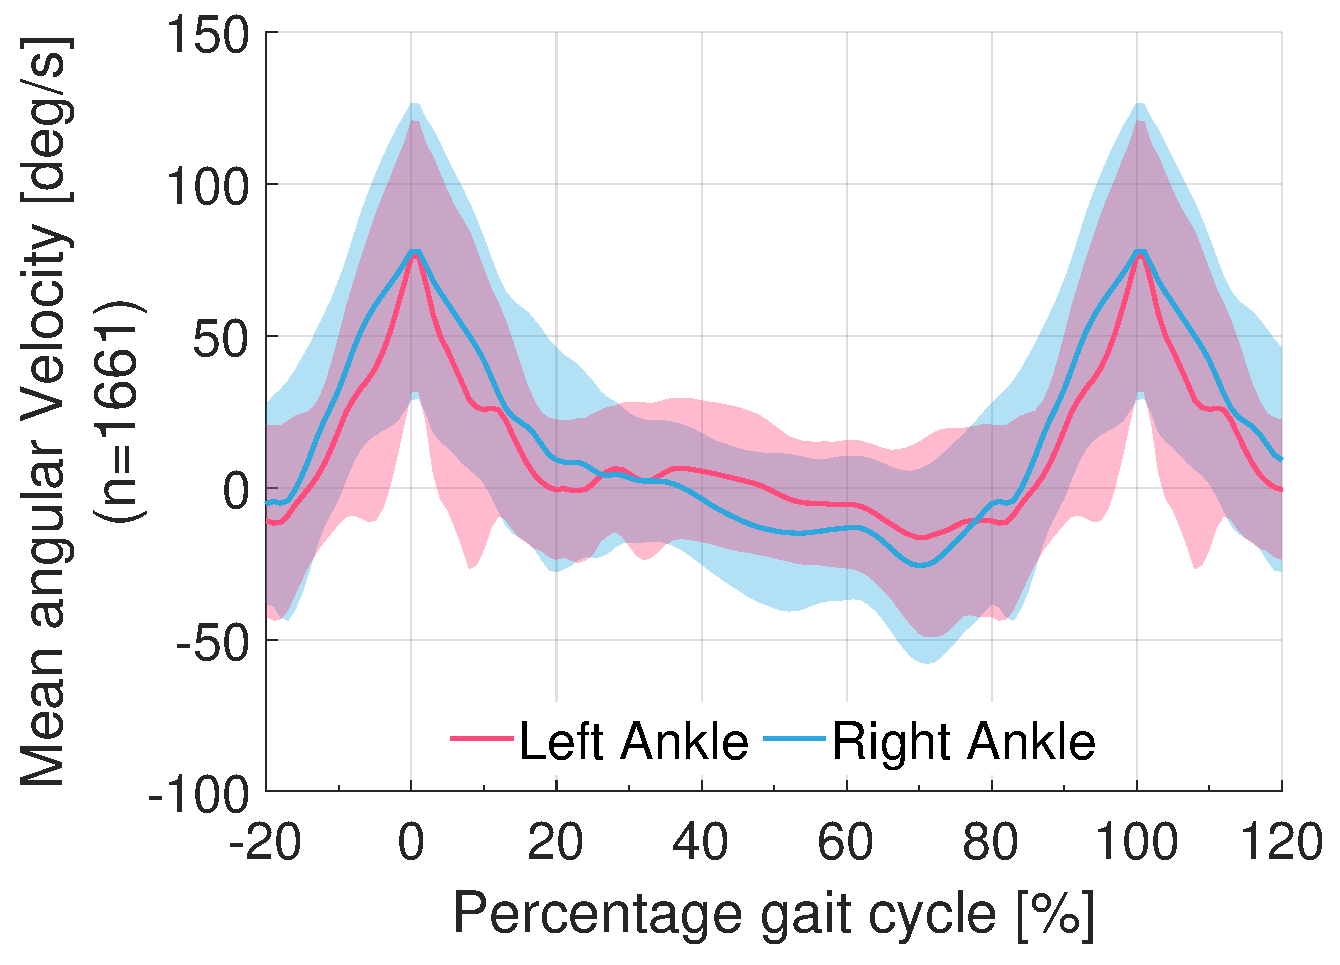
\includegraphics[width=0.275\linewidth]{content/5-Personalisation/Gyro_Trends_For_Targets/ch5_gait_trends_subject_01_activity_ramp_up.pdf} & 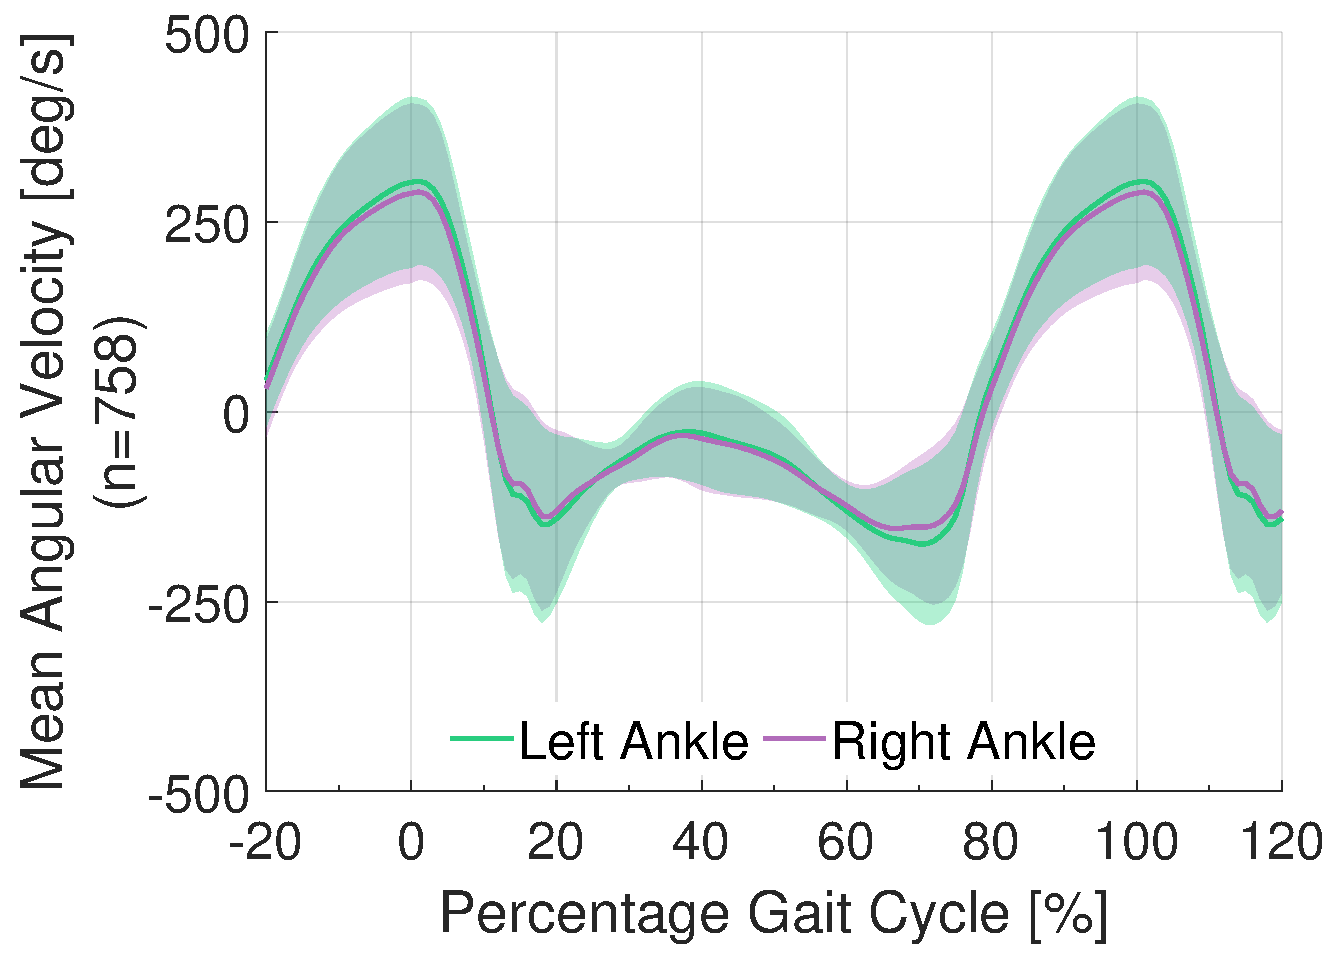
\includegraphics[width=0.275\linewidth]{content/5-Personalisation/Gyro_Trends_For_Targets/ch5_gait_trends_subject_03_activity_ramp_up.pdf} &
        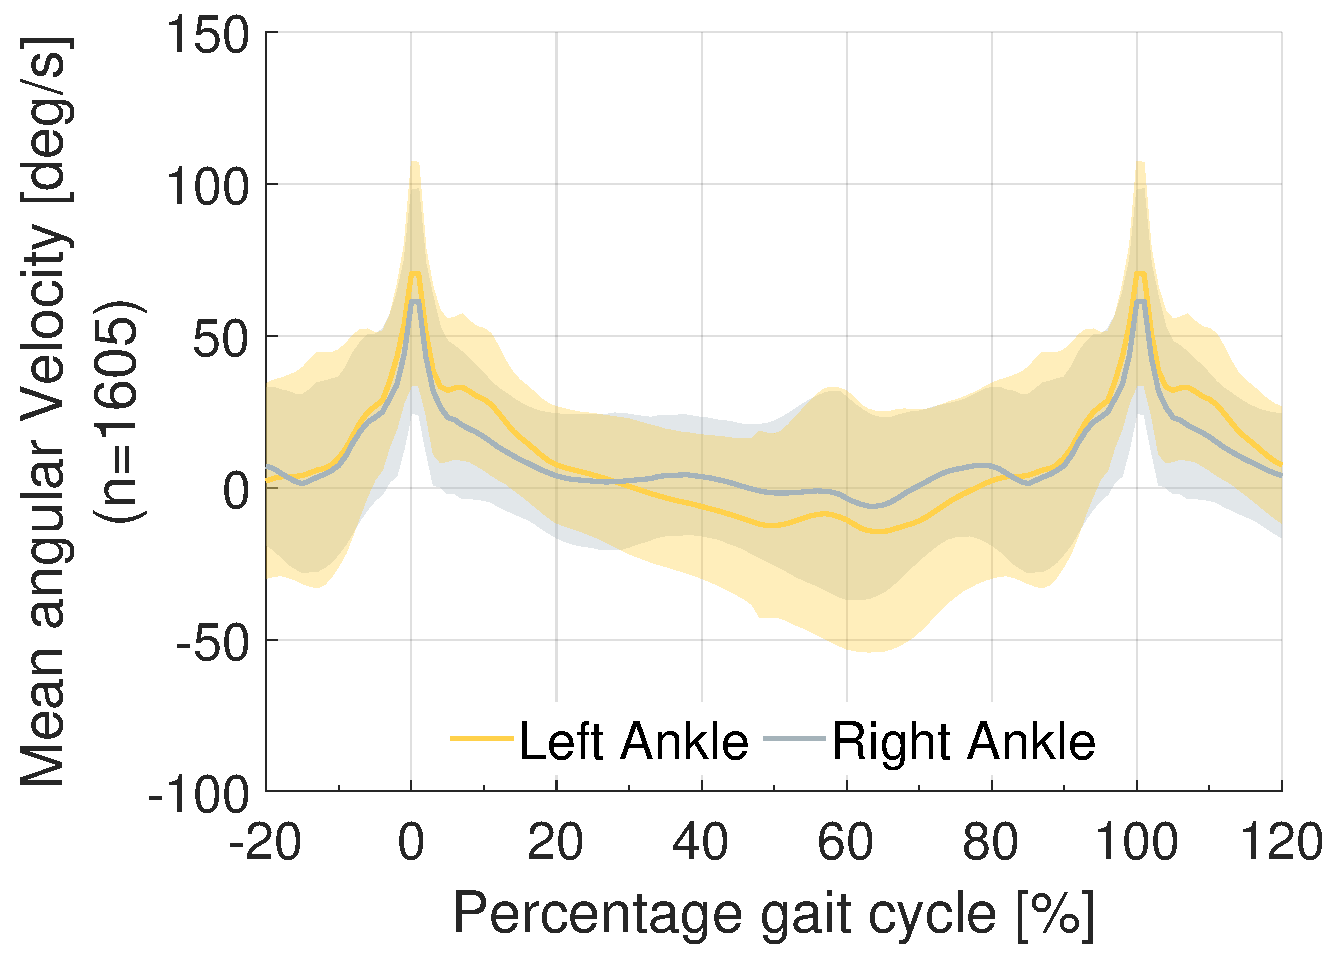
\includegraphics[width=0.275\linewidth]{content/5-Personalisation/Gyro_Trends_For_Targets/ch5_gait_trends_subject_09_activity_ramp_up.pdf} \\
        \rotatebox{90}{\quad \textbf{\glsentrylong{rd}}} & 
        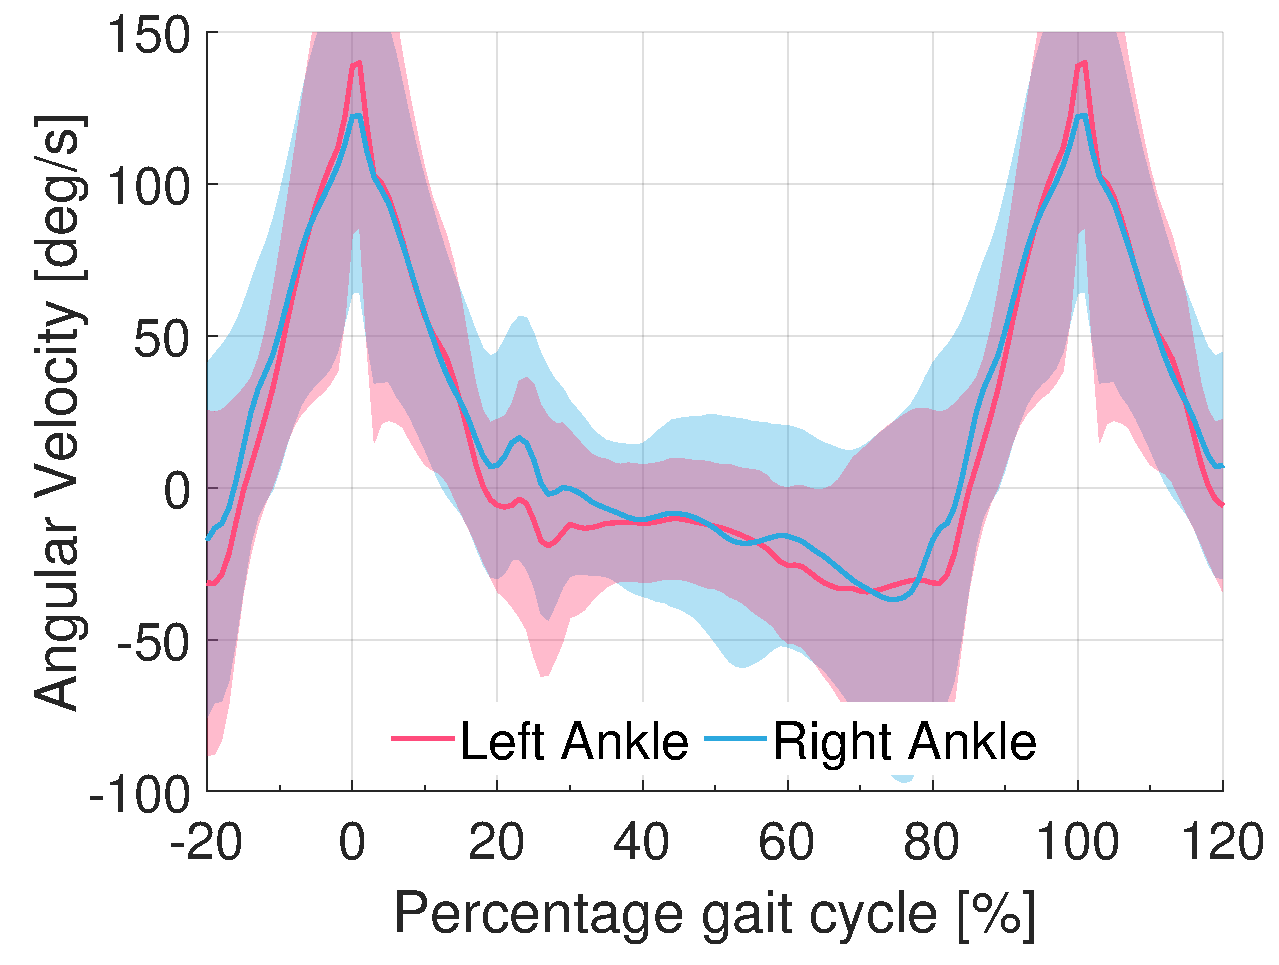
\includegraphics[width=0.275\linewidth]{content/5-Personalisation/Gyro_Trends_For_Targets/ch5_gait_trends_subject_01_activity_ramp_down.pdf} & 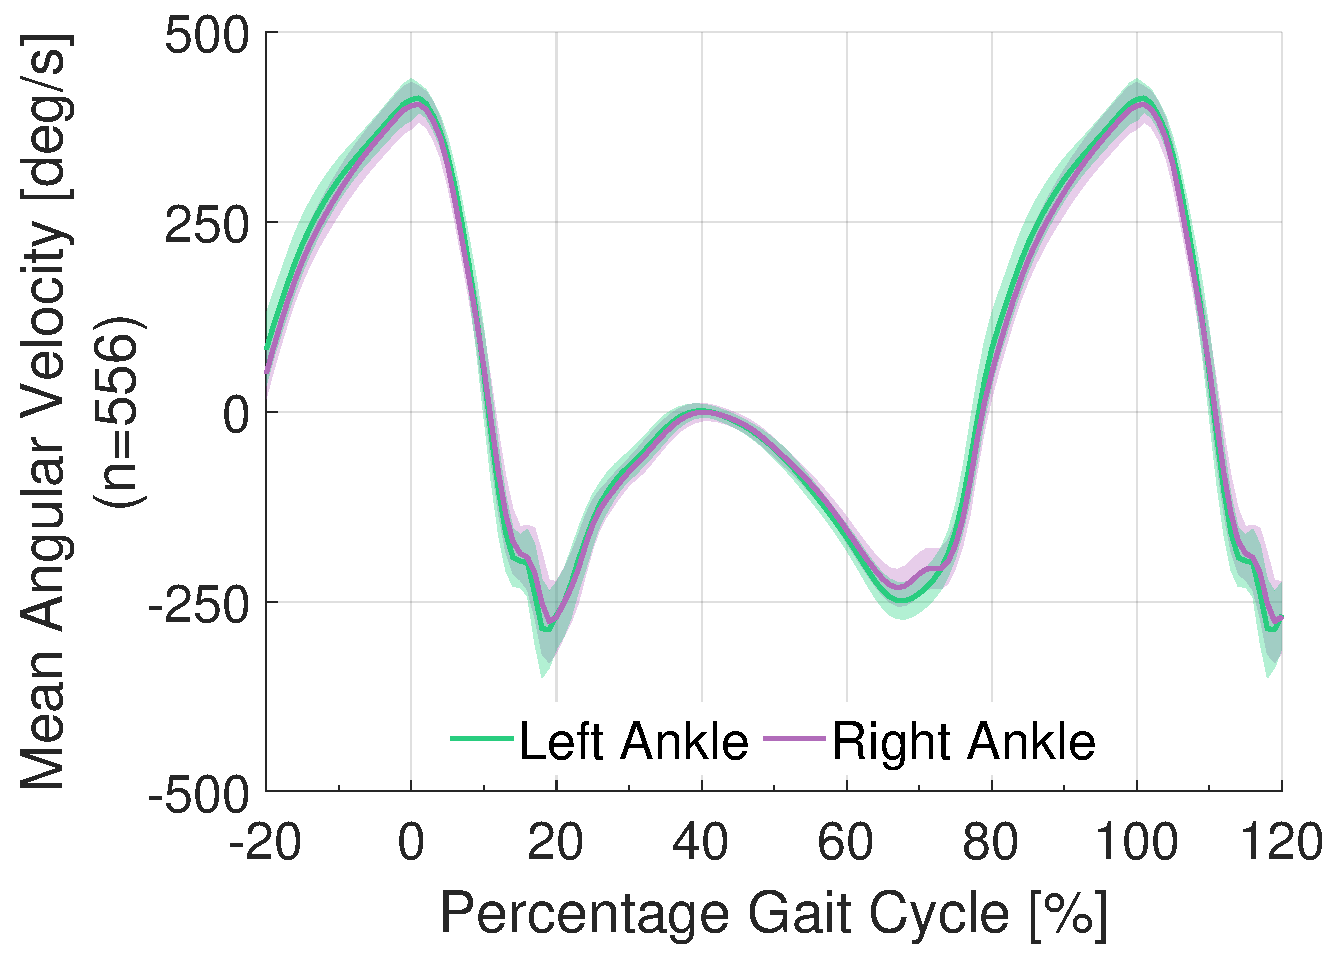
\includegraphics[width=0.275\linewidth]{content/5-Personalisation/Gyro_Trends_For_Targets/ch5_gait_trends_subject_03_activity_ramp_down.pdf} &
        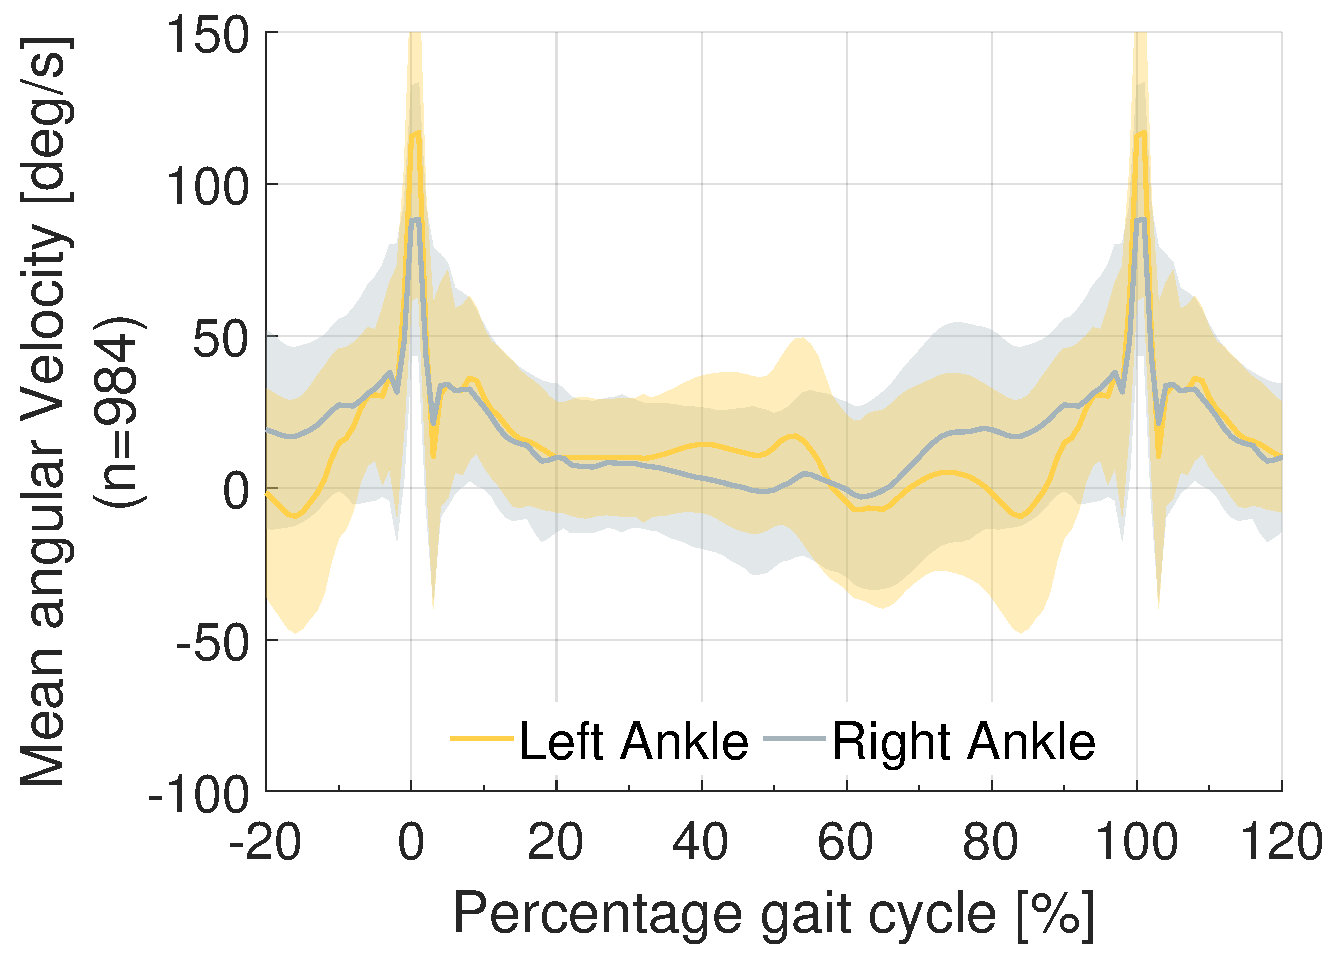
\includegraphics[width=0.275\linewidth]{content/5-Personalisation/Gyro_Trends_For_Targets/ch5_gait_trends_subject_09_activity_ramp_down.pdf} \\
        \rotatebox{90}{~\quad \textbf{\glsentrylong{sa}}} & 
        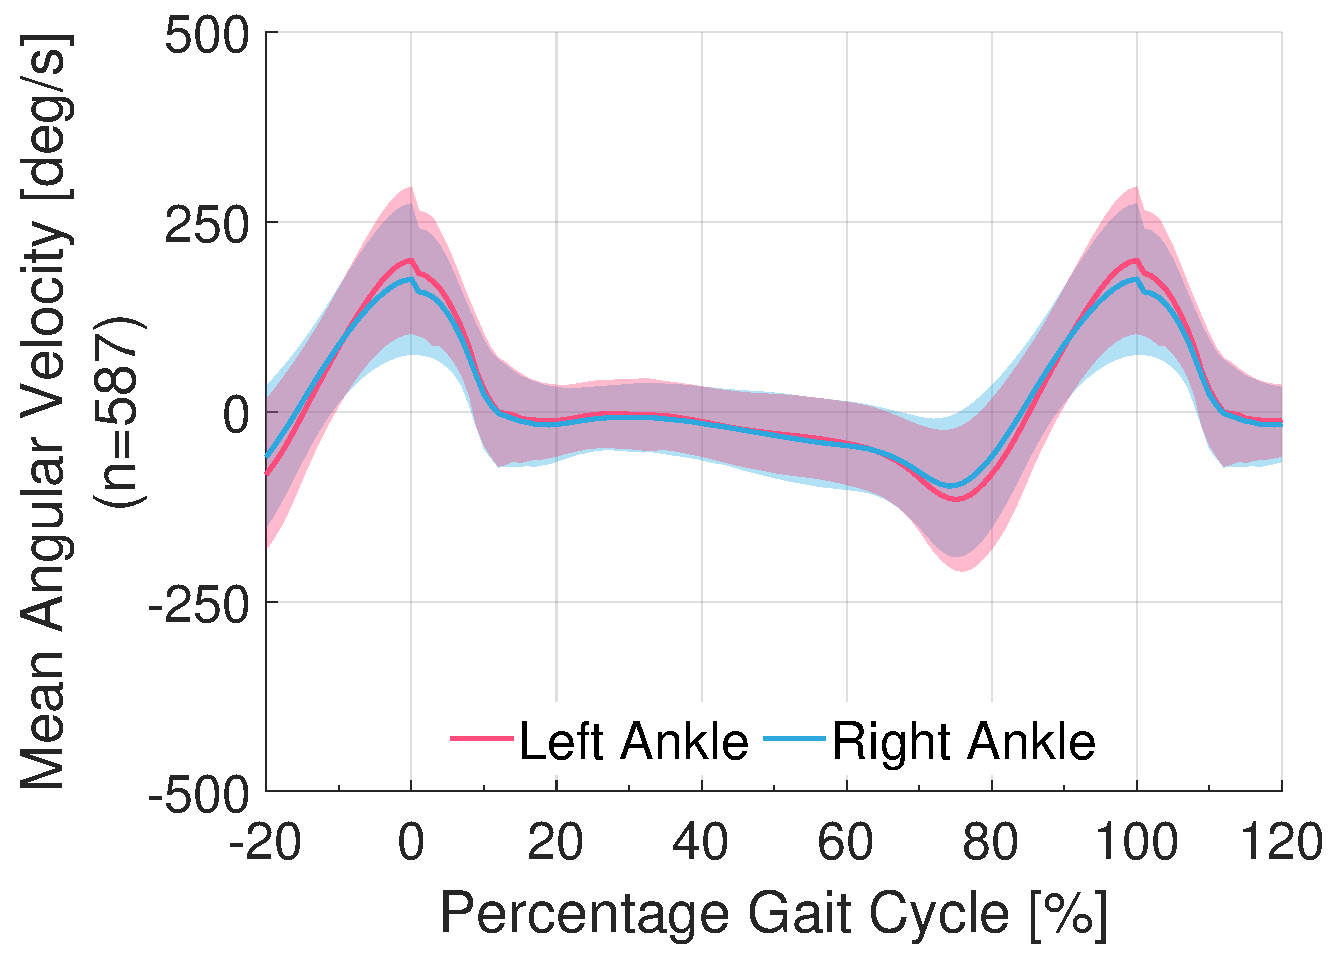
\includegraphics[width=0.275\linewidth]{content/5-Personalisation/Gyro_Trends_For_Targets/ch5_gait_trends_subject_01_activity_stair_up.pdf} & 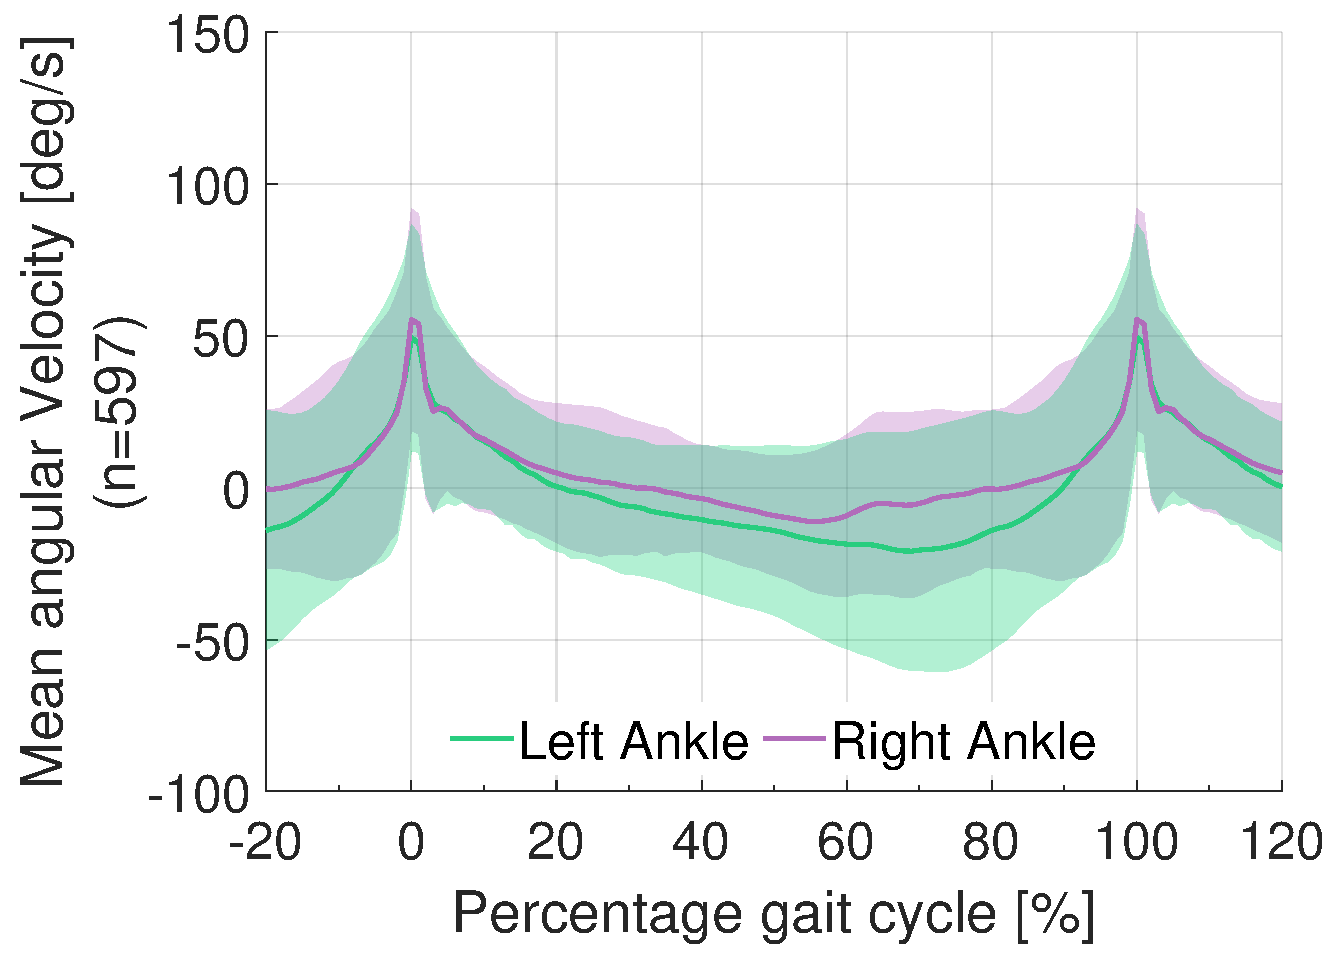
\includegraphics[width=0.275\linewidth]{content/5-Personalisation/Gyro_Trends_For_Targets/ch5_gait_trends_subject_03_activity_stair_up.pdf} &
        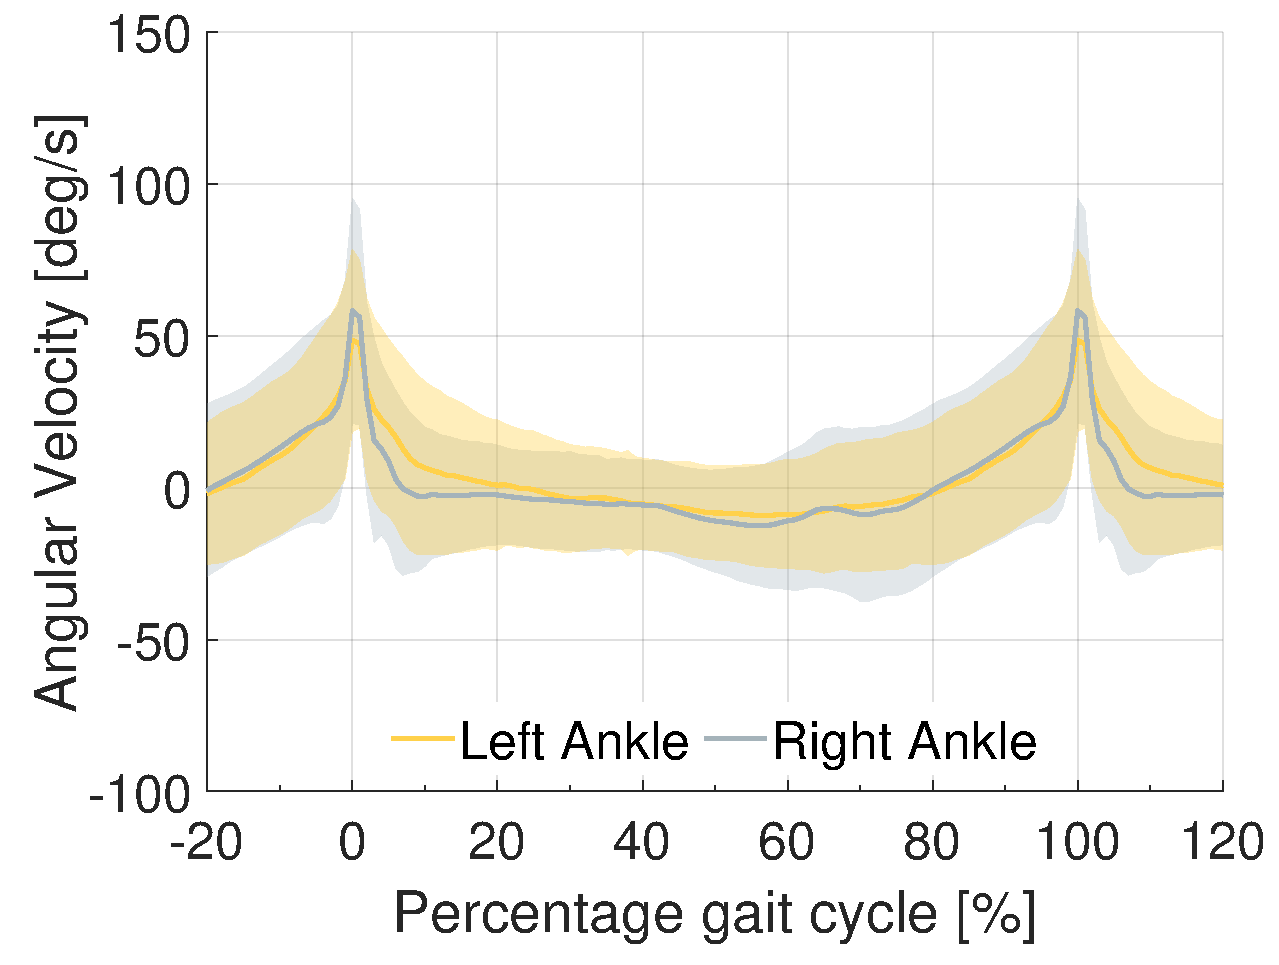
\includegraphics[width=0.275\linewidth]{content/5-Personalisation/Gyro_Trends_For_Targets/ch5_gait_trends_subject_09_activity_stair_up.pdf} \\
        \rotatebox{90}{\quad \textbf{\glsentrylong{sd}}} & 
        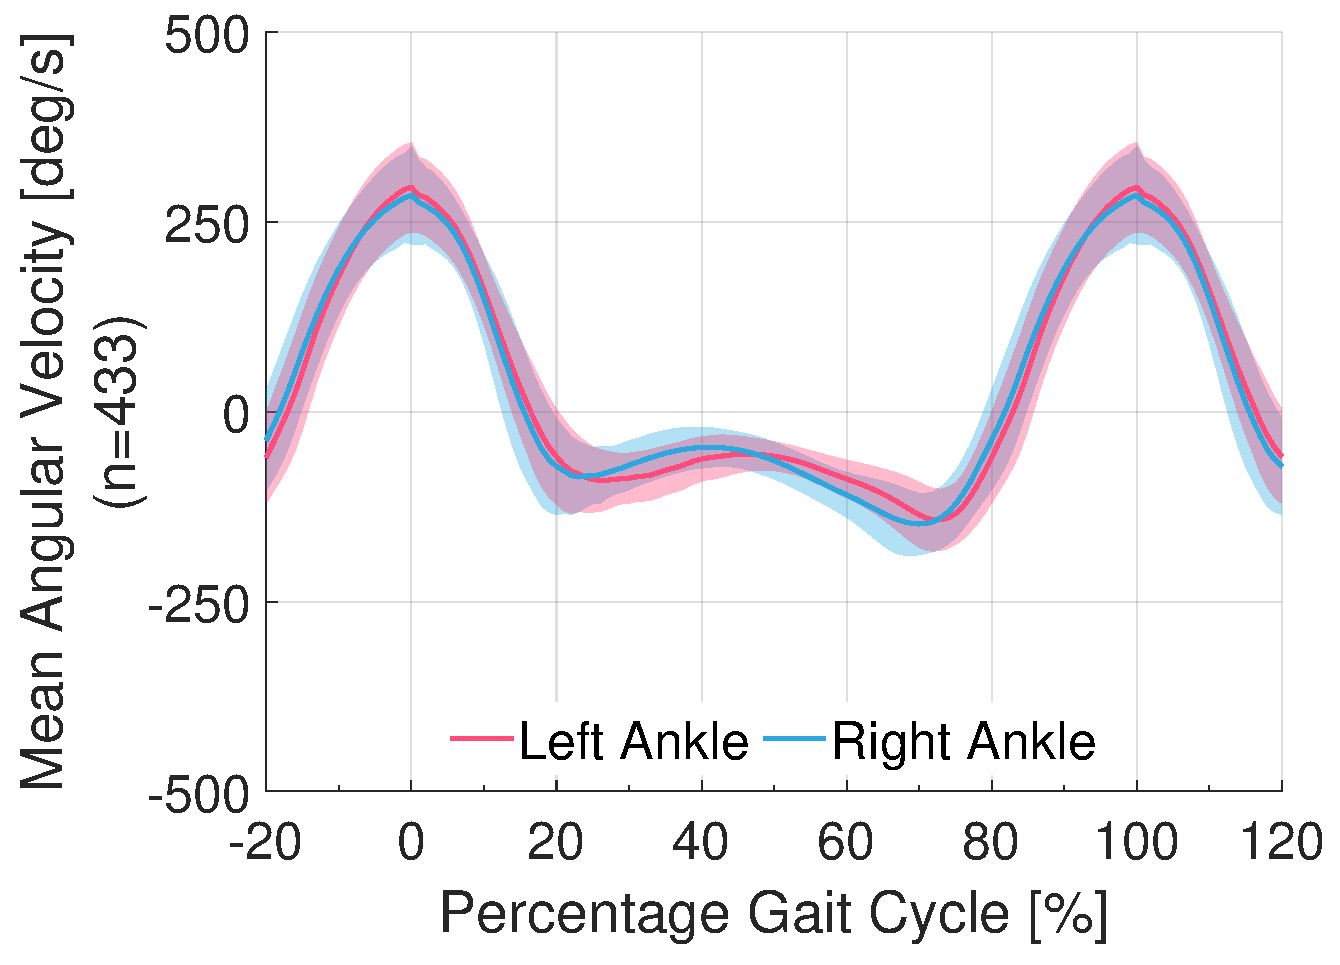
\includegraphics[width=0.275\linewidth]{content/5-Personalisation/Gyro_Trends_For_Targets/ch5_gait_trends_subject_01_activity_stair_down.pdf} & 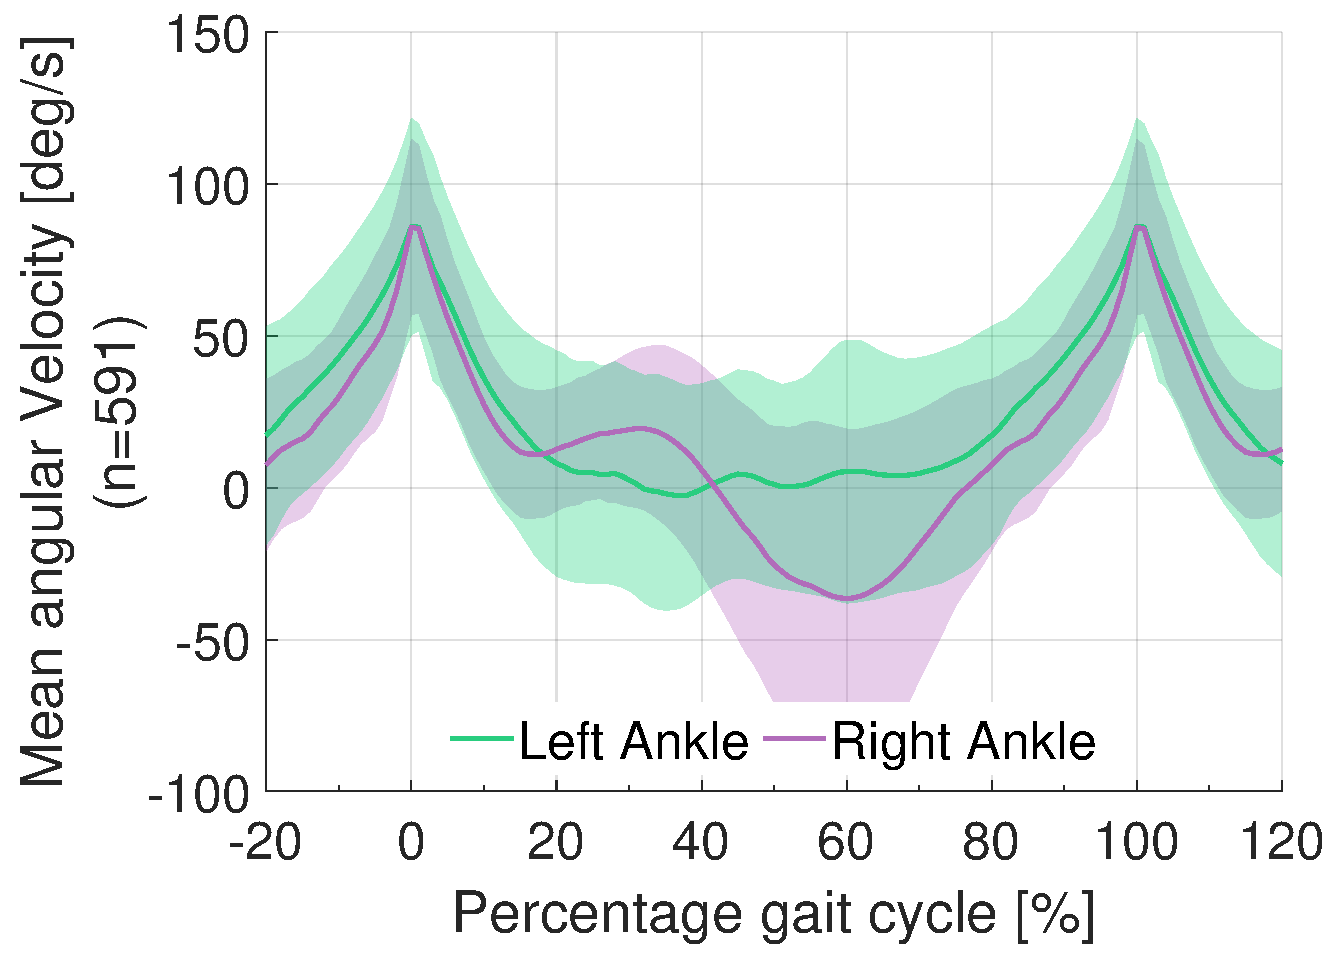
\includegraphics[width=0.275\linewidth]{content/5-Personalisation/Gyro_Trends_For_Targets/ch5_gait_trends_subject_03_activity_stair_down.pdf} &
        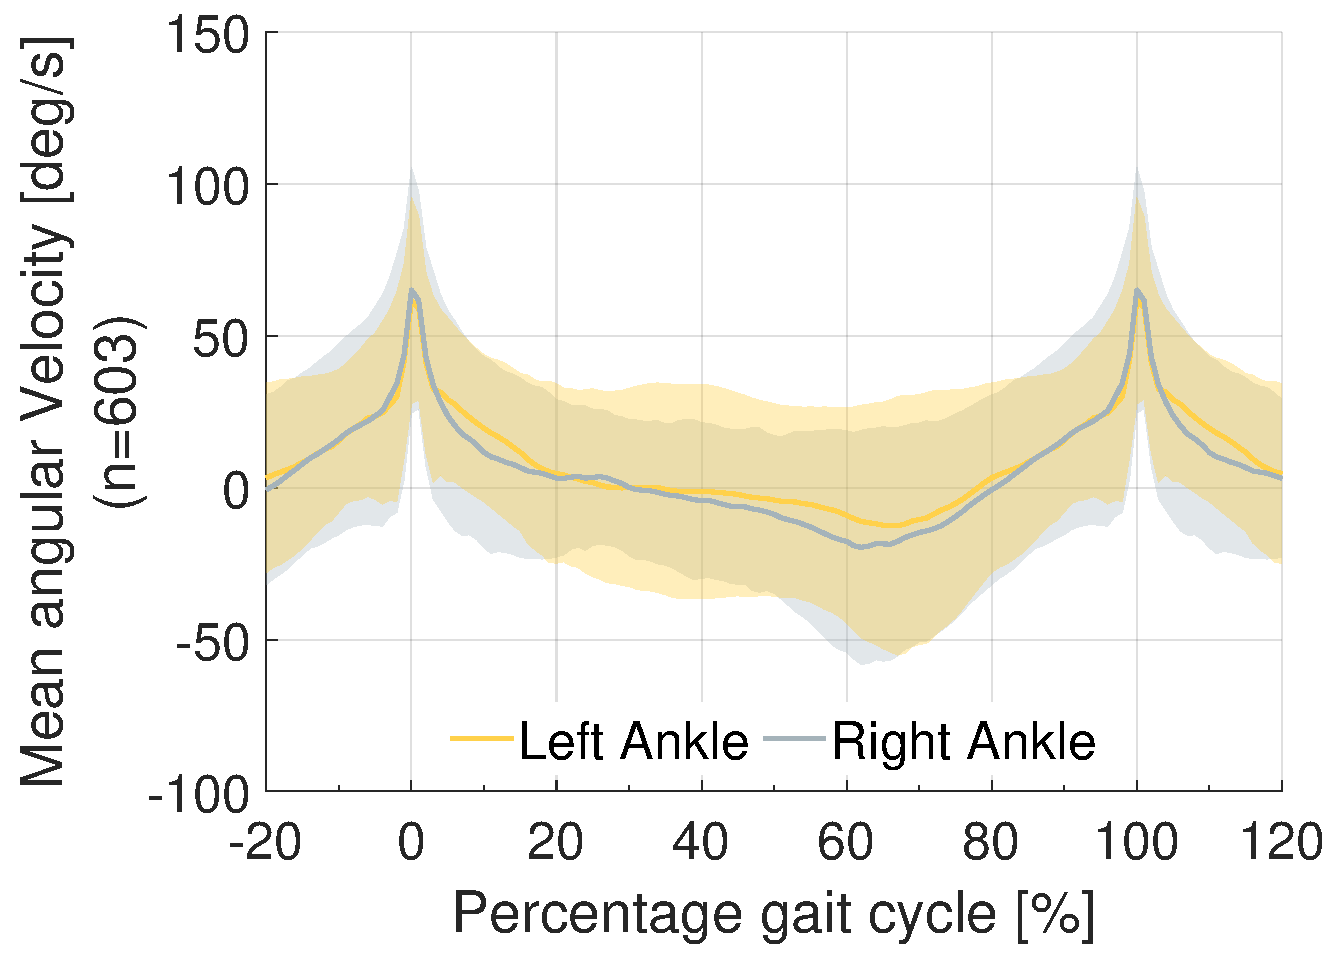
\includegraphics[width=0.275\linewidth]{content/5-Personalisation/Gyro_Trends_For_Targets/ch5_gait_trends_subject_09_activity_stair_down.pdf} \\
    \end{tabular}
    \centering
    \caption[Angular velocity of the shank in the Saggital Plane during different activities for the three target subject]{Angular velocity of the shank in the Saggital Plane during different activities for the three target subject. The solid line shows the mean angular velocity for all steps recorded for each activity. The filled area represents the standard deviation. 0\% gait cycle is taken as peak swing for simplicity of calculation. The red, green and yellow lines are for the left ankles of Subjects 1, 3 and 9 respectively. The blue, purple and grey lines show the right ankles of Subjects 1, 3 and 9 respectively.}
    \label{fig:personalistaion_target_subjects_gyro_trends}
\end{figure}

\subsection{Data Division}
The HAR data set is made of a series of continuous recordings which may cover multiple different activities and environments. Developing an effective method for dividing this data will be critical to demonstrating the effectiveness of personalisation.

It is highly likely to suffer from poor distribution of classes since activities such as walking are far more prevalent than climbing stairs. As \acrshort{ml} methods perform best using balanced data sets, this must be corrected. Additionally, in order for the test set to represent a novel environment, the training data sets should ideally not include any data from the same environment. Therefore each unique episode should only be used once across the training and test data sets. Finally the data division method should allow for multiple repeatable unique sets to be constructed to allow for cross-validation of performance. Achieving all these requirements means that the recordings cannot simply be divided by time.

The proposed approach is to divide the continuous data of each subject into episodes, each containing one continuous period of activity. Episodes can then be combined to form the three independent data sets. Each episode is only used once, any excess episodes are discarded. To balance the number of classes, excess windows are discarded randomly from all episodes. To produce cross-validation sets the starting order of the episodes can be shuffled. Figure \ref{fig:methods-per-episode-data-division} illustrates the process of forming the three data sets.

 \begin{figure}[hbt]
     \centering
     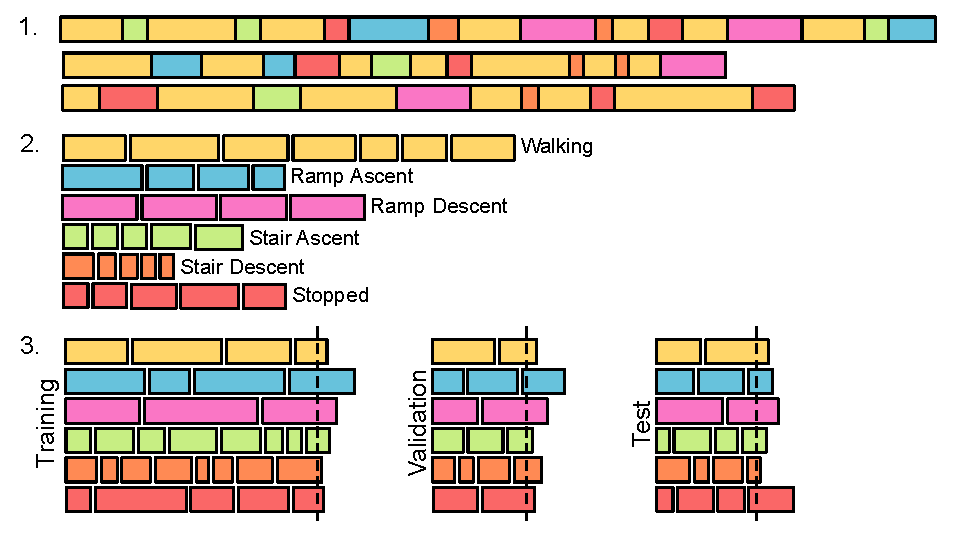
\includegraphics[width=0.9\textwidth]{content/3-Methods/Episode_Division.pdf}
     \caption[Per-episode data division]{Per-episode data division. Step 1 -- Labelled data files for a participant are loaded. Step 2 -- Episodes of the same activity are grouped together. Step 3 -- Training, Validation and Test sets are formed by stacking episodes until the required window quantity reached.}
     \label{fig:methods-per-episode-data-division}
 \end{figure}
 
%BOOKMARK (SM) - PROOF READ UP TO HERE
For all experiments the test sets will contain 5000 windows of target data. Training/validation set will vary in length. For conciseness the number of training windows will be presented as the sum of both training and validation windows. These will always be in the ratio 70:30. 

Each experiment will be repeated multiple time with episodes randomly shuffled between each to improve statistical certainty. The shuffling will be repeatable and test data will always be drawn first to ensure a consistent test set.

The time in seconds can be calculated using Equation \ref{eqn:episode_set_length_seconds}, where $T$ is total set length in seconds, $f_s$ is the sampling frequency, $s_k$ is the window skip value, $n_w$ is the number of windows, $l_w$ is the window size, and $n_e$ is the number of episodes included in the set.

\begin{equation}
    T = \frac{1}{f_s}(s_k n_w + l_w n_e)
    \label{eqn:episode_set_length_seconds}
\end{equation}

Calculating the actual quantity of data used in seconds is non-trivial as some windows may be dropped during class balancing. Assuming no windows are dropped and only one episode is used 5000 windows uses a minimum of 151 seconds for each class. $l_w$ set to 128, $f_s$ set to 100Hz, and $s_k$ equal to three.

%--------------------------------
% Machine learning methods
\subsection{\glsentrylong{ml} Methods}
Two personalisation methods will be evaluated -- data supplementation and transfer learning. These will be compared against two baselines, a model trained using only target training data, and a general subject agnostic model.

The data supplementation technique will mix source and target data to produce a larger training set. This will then be used to train a new classifier from scratch. The additional data will be selected randomly without attempting to match similar subjects. The amount of both source and target data will be varied to investigate the impact of both.

The transfer learning approach will fine-tuned a set of base general models using data from a target subject. The base models will be generated by training a model from scratch using the full source data excluding the three target subjects. Five base model will be produced, by randomly shuffling the training and validation.

Personalisation will be performed by additional training using just target data. The amount of target training data used will be varied to asses the impact of this of classification performance. Three different training configurations will be tested, each configuration will vary by which layers are trained. For the first configuration all layers will be fine-tuned, the second and third method will train only the \acrshort{lstm} and dense layers respectively.

The same \acrshort{lstm} architecture will be used throughout all experiments shown in Figure \ref{fig:ch5_illustration_of_base_LSTM_model}. This is the same architecture as used in Chapter \ref{chp:lstm-general}. The first has an \acrshort{lstm} layer than takes a 128 x 6 input of raw \acrshort{imu} data. The \acrshort{lstm} layer can be a varying number of units wide but will always be 128 units long. The full output of this layer is then passed to a dense late fusion layer before been passed through a \acrshort{relu} classifier. TensorFlow allocates 4992 parameters to a 32 unit 128 long LSTM layer and 24582 parameters to the Dense layer.

\begin{figure}[htbp]
    \centering
    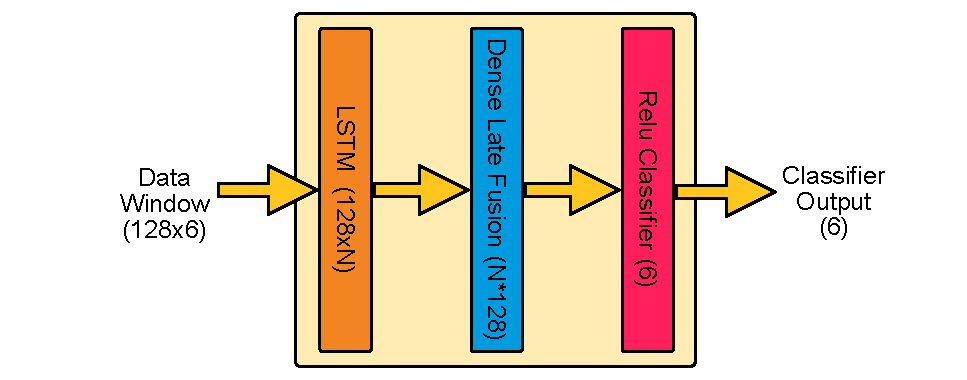
\includegraphics[width=0.8\textwidth]{content/5-Personalisation/ch5_lstm_architecture.pdf}
    \caption[Illustration of \glsentryshort{lstm} machine learning model architecture]{Illustration of \acrshort{lstm} machine learning model architecture}
    \label{fig:ch5_illustration_of_base_LSTM_model}
\end{figure}


All training will be undertake using the same methods as described in Chapter \ref{chp:lstm-general}. The full set of windows will be passed thought the training systems in mini-batches of 100 windows. After every epoch the validation set will be used to evaluate the performance of the model. When the categorical loss of the validation set stagnates for more than 3 epochs training will be stopped. All training hyper-parameters were tune empirically.

Model performance will be assessed primarily by the classification accuracy using the unseen test data set. Additionally measures include the number of epochs, training time and quantity of training data required. These will aim in determining the computationally/data efficient. By using comparison against the baselines it will be possible to determine if these methods are of benefit.


%-------------------------------------------------------------------------------
\section{Baseline Model Performance}
\label{sec:personalisation-baseline-model-results}
To determine if personalisation has resulted in an improvement a performance baseline is required. Two baselines will be generated for each target subject. These will be the accuracy of a general model for the target, and the accuracy of a model trained using only target data. If performance of the personalisation methods do not exceed the baselines there is no benefit in them. The performance of both baselines is presented within this section.

% Performance of the trained general models with no fine-tuning
For the first baseline the classification accuracy of the general models when presented with the test data sets was evaluated. The average accuracy of the five models was $75.0\%\pm2.3$ for Subject 1, $63.9\%\pm2.9$ for Subject 3 and $77.4\%\pm5.1$ for Subject 9. The confusion matrices for each subject is presented in Table \ref{tab:ch5-general-model-confusion-matrix}. Performance is averaged across the five general models and five test sets. Each cell contains the percentage of total predictions of each class.

Table \ref{tab:ch5-general-model-confusion-matrix} shows that each target subject struggles at different classes. This is as you would expect given the likely differences in gait characteristics.

% Confusion matrix for general model
\begin{table}[p]
    \centering
    \caption[Confusion matrix of a general model presented with target subject test data]{Confusion matrix of a general model presented with target subject test data. Columns represent the prediction labels and the rows represent the real labels. Each value represent the percentage of total predictions of that class. (\acrfull{ra}, \acrfull{rd}, \acrfull{sa}, \acrfull{sd})}
    \label{tab:ch5-general-model-confusion-matrix}
    \begin{subtable}{\textwidth}
    \caption{Subject 1}
    \begin{tabularx}{\textwidth}{ccYYYYYY}
        \noalign{\hrule height 1.5pt}
         & & \multicolumn{6}{c}{\textbf{Predicted Classes}} \\
         \hline
         & & WALK & \glsentryshort{ra} & \glsentryshort{rd} & \glsentryshort{sa} & \glsentryshort{sd} & STOP \\
         \multirow{6}{*}{\rotatebox{90}{\textbf{True Classes}}} 
         & WALK               & 37.9 & 26.9 & 24.5 & 0.1 & 6.2 & 6.3 \\
         & \glsentryshort{ra} & 57.9 & 65.3 & 1.2 & 1.0 & 0.2 & 0.0 \\
         & \glsentryshort{rd} & 2.4 & 0.9 & 72.8 & 0.0 & 3.7 & 0.5 \\
         & \glsentryshort{sa} & 0.5 & 5.9 & 0.0 & 98.6 & 1.3 & 2.0 \\
         & \glsentryshort{sd} & 1.1 & 0.8 & 1.5 & 0.2 & 88.6 & 5.8 \\
         & STOP               & 0.2 & 0.3 & 0.0 & 0.0 & 0.0 & 85.4 \\
         \noalign{\hrule height 1.5pt} \\
    \end{tabularx}
    \end{subtable}
    \begin{subtable}{\textwidth}
    \caption{Subject 3}
    \begin{tabularx}{\textwidth}{ccYYYYYY}
        \noalign{\hrule height 1.5pt}
         & & \multicolumn{6}{c}{\textbf{Predicted Classes}} \\
         \hline
         & & WALK & \glsentryshort{ra} & \glsentryshort{rd} & \glsentryshort{sa} & \glsentryshort{sd} & STOP \\
         \multirow{6}{*}{\rotatebox{90}{\textbf{True Classes}}} 
         & WALK               & 27.4 & 29.5 & 1.7 & 4.3 & 5.4 & 19.6 \\
         & \glsentryshort{ra} & 40.3 & 70.2 & 1.0 & 0.2 & 0.1 & 2.3 \\
         & \glsentryshort{rd} & 31.6 & 0.2 & 94.3 & 0.5 & 8.2 & 0.9 \\
         & \glsentryshort{sa} & 0.4 & 0.1 & 0.3 & 94.9 & 0.7 & 0.9 \\
         & \glsentryshort{sd} & 0.3 & 0.0 & 2.7 & 0.1 & 85.6 & 0.0 \\
         & STOP               & 0.0 & 0.0 & 0.0 & 0.0 & 0.0 & 76.3 \\
         \noalign{\hrule height 1.5pt} \\
    \end{tabularx}
    \end{subtable}
    \begin{subtable}{\textwidth}
    \caption{Subject 9}
    \begin{tabularx}{\textwidth}{ccYYYYYY}
        \noalign{\hrule height 1.5pt}
         & & \multicolumn{6}{c}{\textbf{Predicted Classes}} \\
         \hline
         & & WALK & \glsentryshort{ra} & \glsentryshort{rd} & \glsentryshort{sa} & \glsentryshort{sd} & STOP \\
         \multirow{6}{*}{\rotatebox{90}{\textbf{True Classes}}} 
         & WALK               & 59.6 & 8.5 & 10.7 & 0.5 & 9.3 & 1.3 \\
         & \glsentryshort{ra} & 13.3 & 89.2 & 0.2 & 14.6 & 2.5 & 1.0 \\
         & \glsentryshort{rd} & 17.7 & 0.0 & 84.3 & 0.0 & 15.7 & 0.0 \\
         & \glsentryshort{sa} & 4.7 & 1.7 & 0.0 & 78.3 & 1.2 & 2.1 \\
         & \glsentryshort{sd} & 4.7 & 0.5 & 4.8 & 0.5 & 71.4 & 2.9 \\
         & STOP               & 0.1 & 0.0 & 0.0 & 6.0 & 0.0 & 92.6 \\
         \noalign{\hrule height 1.5pt} \\
    \end{tabularx}
    \end{subtable}
\end{table}

To determine a baseline for models trained with only target training data LSTM models of different shapes were trained using increasing amounts of target data. Figure \ref{fig:ch5_bespoke_mode_classification} shows the classification performance for each of subject using different quantities of target data windows for 6, 16, 32 and 64 unit \acrshort{lstm} networks. The full data tables are available in Appendix \ref{chp:tables-of-results} Section \ref{sec:appendix-a-model-performance-bespoke}.

% Confusion matrix for bespoke model
\begin{table}[p]
    \centering
    \caption[confusion matrix for a bespoke \acrshort{lstm} model presented with target subject test data]{confusion matrix for a bespoke \acrshort{lstm} model presented with target subject test data. The 32 unit \acrshort{lstm} model was trained with 15000 target data window. Columns represent the prediction labels and the rows represent the real labels. Each value represent the percentage of total predictions of that class. (\acrfull{ra}, \acrfull{rd}, \acrfull{sa}, \acrfull{sd})}
    \label{tab:ch5-bespoke-model-confusion-matrix}
    \begin{subtable}{\textwidth}
    \caption{Subject 1}
    \begin{tabularx}{\textwidth}{ccYYYYYY}
        \noalign{\hrule height 1.5pt}
         & & \multicolumn{6}{c}{\textbf{Predicted Classes}} \\
         \hline
         & & WALK & \glsentryshort{ra} & \glsentryshort{rd} & \glsentryshort{sa} & \glsentryshort{sd} & STOP \\
         \multirow{6}{*}{\rotatebox{90}{\textbf{True Classes}}} 
         & WALK               & 71.3 & 20.6 & 18.1 & 0.4 & 1.9 & 2.7 \\
         & \glsentryshort{ra} & 25.9 & 72.4 & 0.0 & 0.0 & 0.0 & 0.0 \\
         & \glsentryshort{rd} & 1.2 & 0.0 & 80.0 & 0.2 & 6.2 & 0.0 \\
         & \glsentryshort{sa} & 0.9 & 5.6 & 0.2 & 92.9 & 5.2 & 0.2 \\
         & \glsentryshort{sd} & 0.8 & 1.2 & 1.7 & 4.5 & 86.7 & 1.7 \\
         & STOP               & 0.1 & 0.1 & 0.0 & 2.0 & 0.1 & 95.4 \\
         \noalign{\hrule height 1.5pt} \\
    \end{tabularx}
    \end{subtable}
    \begin{subtable}{\textwidth}
    \caption{Subject 3}
    \begin{tabularx}{\textwidth}{ccYYYYYY}
        \noalign{\hrule height 1.5pt}
         & & \multicolumn{6}{c}{\textbf{Predicted Classes}} \\
         \hline
         & & WALK & \glsentryshort{ra} & \glsentryshort{rd} & \glsentryshort{sa} & \glsentryshort{sd} & STOP \\
         \multirow{6}{*}{\rotatebox{90}{\textbf{True Classes}}} 
         & WALK               & 50.3 & 3.3 & 4.2 & 0.2 & 4.1 & 3.1 \\
         & \glsentryshort{ra} & 32.3 & 52.1 & 0.3 & 0.0 & 0.0 & 0.0 \\
         & \glsentryshort{rd} & 16.5 & 43.5 & 92.1 & 0.1 & 0.5 & 0.0 \\
         & \glsentryshort{sa} & 0.5 & 0.8 & 0.2 & 99.2 & 1.5 & 1.0 \\
         & \glsentryshort{sd} & 0.2 & 0.2 & 3.1 & 0.5 & 94.0 & 0.1 \\
         & STOP               & 0.1 & 0.0 & 0.0 & 0.0 & 0.1 & 95.7 \\
         \noalign{\hrule height 1.5pt} \\
    \end{tabularx}
    \end{subtable}
    \begin{subtable}{\textwidth}
    \caption{Subject 9}
    \begin{tabularx}{\textwidth}{ccYYYYYY}
        \noalign{\hrule height 1.5pt}
         & & \multicolumn{6}{c}{\textbf{Predicted Classes}} \\
         \hline
         & & WALK & \glsentryshort{ra} & \glsentryshort{rd} & \glsentryshort{sa} & \glsentryshort{sd} & STOP \\
         \multirow{6}{*}{\rotatebox{90}{\textbf{True Classes}}} 
         & WALK               & 90.4 & 7.6 & 6.3 & 2.0 & 2.7 & 0.0 \\
         & \glsentryshort{ra} & 2.2 & 82.5 & 0.1 & 1.4 & 0.1 & 0.0 \\
         & \glsentryshort{rd} & 5.6 & 7.4 & 85.1 & 2.1 & 8.8 & 0.0 \\
         & \glsentryshort{sa} & 1.0 & 1.7 & 0.6 & 92.8 & 4.7 & 0.1 \\
         & \glsentryshort{sd} & 0.8 & 0.6 & 8.0 & 1.6 & 83.4 & 0.7 \\
         & STOP               & 0.1 & 0.2 & 0.0 & 0.2 & 0.4 & 99.2 \\
         \noalign{\hrule height 1.5pt} \\
    \end{tabularx}
    \end{subtable}
\end{table}

% Classification performance
\begin{figure}[p]
    \centering
    \begin{subfigure}[b]{\textwidth}
        \centering
        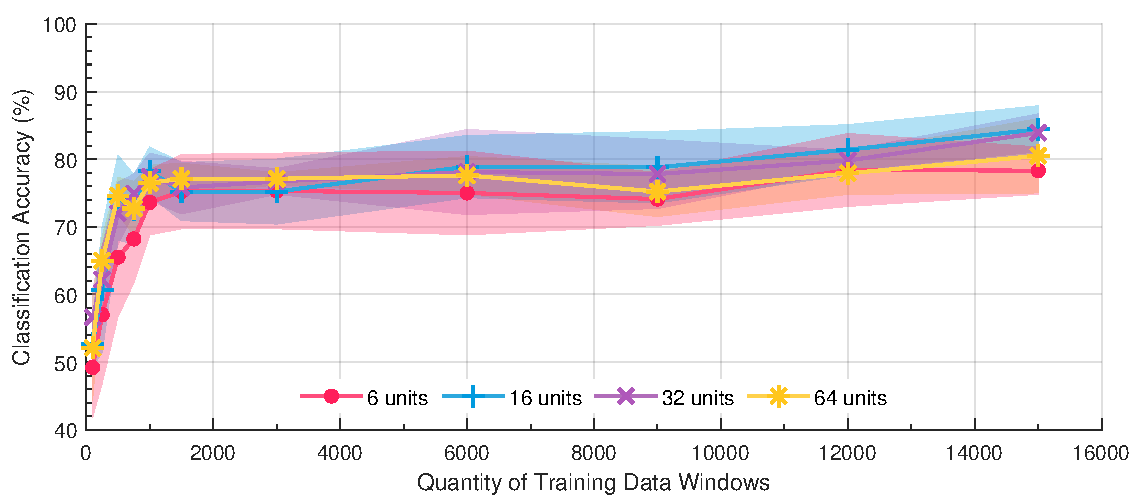
\includegraphics[width=\textwidth]{content/5-Personalisation/Bespoke_Target/ch5_bespoke_target_model_subject_1.pdf}
        \caption{Subject 1}
        \label{fig:ch5_6_unit_bespoke_model}
    \end{subfigure}
    \begin{subfigure}[b]{\textwidth}
        \centering
        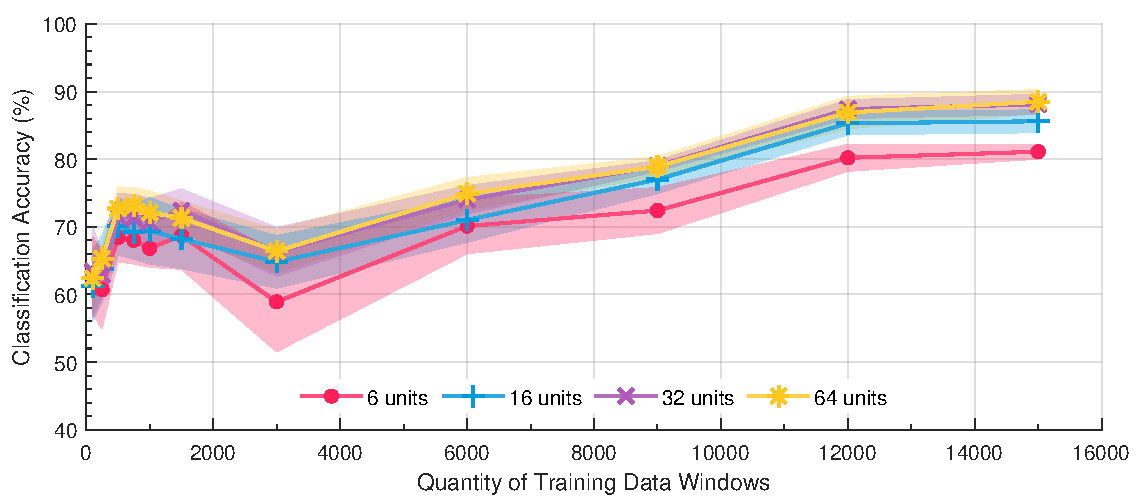
\includegraphics[width=\textwidth]{content/5-Personalisation/Bespoke_Target/ch5_bespoke_target_model_subject_3.pdf}
        \caption{Subject 3}
        \label{fig:ch5_16_unit_bespoke_model}
    \end{subfigure}
    \caption[Classification performance of different size \glsentryshort{lstm} networks trained with varying amount of target subject data]{Classification performance of different size \acrshort{lstm} networks trained with varying amount of target subject data. The solid lines represent the mean of all models trained, the filled area represents the standard deviation $(n=10)$. Each line show the classification performance for a different number of \acrshort{lstm} units. The red dot is 6 units, blue plus 16, purple cross 32 and yellow asterisk 64.}
    \label{fig:ch5_bespoke_mode_classification}
\end{figure}
\begin{figure}[t]\ContinuedFloat
    \begin{subfigure}[b]{\textwidth}
        \centering
        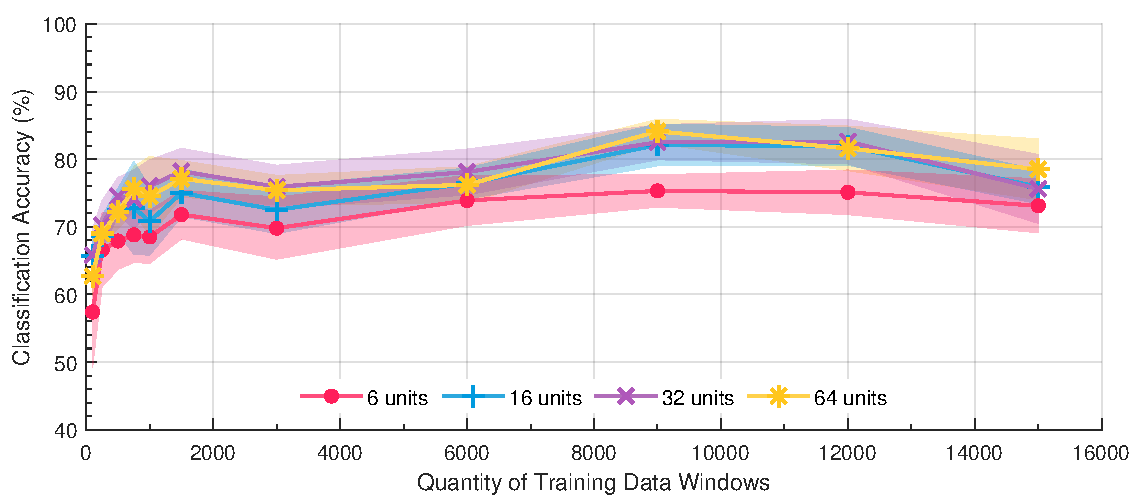
\includegraphics[width=\textwidth]{content/5-Personalisation/Bespoke_Target/ch5_bespoke_target_model_subject_9.pdf}
        \caption{Subject 9}
        \label{fig:ch5_32_unit_bespoke_model}
    \end{subfigure}
    \caption[]{Classification performance of different size \acrshort{lstm} networks trained with varying amount of target subject data (Cont.).}
\end{figure}

%BOOKMARK - (FS) REWRITTEN UP TO HERE
The maximum performance achieved was $84.4\%$ for Subject 1, $88.5\%$ for Subject 3, and $82.6\%$ for Subject 9. This was achieved at 15000 windows for Subjects 1 and 3 but 9000 samples for Subject 9. It's not clear why performance decreased after this point. Performance of the general model is exceeded at around 1500 windows.

The fastest rate of performance improvement was seen early on, from 100 to 1500 data windows. Beyond this there was a more gradual increase in performance. It appears that performance would have continued to improve the maximum number of windows tested. Indicating further data would still improve performance. 

Standard deviation reduced with increasing quantities of data windows indicating more consistent performance across all test sets as as the model was exposed to more data.

The baseline model took on average 8 epochs to train with a 95\textsuperscript{th} percentile of 13

Increasing the number of units in general improved classification performance. This levels off at 32 units. Only the 6 unit model appears to have insufficient learning capacity. Increasing the number of units also reduced the number of epochs required to train the models. Therefore 32 units is likely a good candidate for future models.

The reduction in performance at 3000 samples for Subject 3 is likely due to model exposure to a new environment of data. Performance recovers with increasing amounts of data. Subject 9 also experiences similar drops in performance.

%Why is the model not achieving better performance?
An assessment of where classification errors are occurring can be made by looking at the confusion matrices. Table \ref{tab:ch5-bespoke-model-confusion-matrix} shows confusion matrices for the three targets classifiers created using 15000 training windows. Performance is averaged across the five bespoke models test sets. Each cell contains the percentage of total predictions of each class.

The confusion matrices show that the stop class achieves the highest accuracy, greater than $95\%$ for all subjects. As this is a very distinct class this should be expected. Stairs were also identified fairly accurately with \acrlong{sa} achieving greater than $92\%$ accuracy and \acrlong{sd} greater than $83\%$. The classifier struggled to distinguish walking from, \acrlong{ra} and \acrlong{rd} for all subjects with accuracy as low as $50\%$. 

Comparisons between the two confusion matrices, Tables \ref{tab:ch5-general-model-confusion-matrix} and \ref{tab:ch5-bespoke-model-confusion-matrix} show that each perform better in different classes. Therefore combining the knowledge from both data sources should lead to an improvement in performance.

%-------------------------------------------------------------------------------
\section{Results and Analysis}
\label{sec:model-personalisation-results}
The results and analysis for both personalisation methods, data supplementation and transfer learning, are presented within this section.

%-------------------------------------------------------------------------------
\subsection{Data Supplementation}
A series of \acrshort{lstm} models were trained using different quantities of source and target windows. The experiment aimed to establish if the addition of source data improves the classification performance.

Tables \ref{tab:ch5-mixed-target-and-source-data-subject-01}, \ref{tab:ch5-mixed-target-and-source-data-subject-03} and \ref{tab:ch5-mixed-target-and-source-data-subject-09} present the results data supplementation experiments. Each cell contains the mean classification accuracy for target training and standard deviation. Columns represent different quantities source training windows. Table rows represent different quantities of target training windows. The highest classification accuracy for each quantity of target training windows has been highlighted in bold.

% Fully trained model
% Present performance on this model - Categorical accuracy of training data, learning rate (epochs vs categorical accuracy)
\begin{landscape}
% Subject 01 - classification accuracy for varying source and target data
\begin{table}[p]
    \centering
    \caption[Table of classification accuracy for Subject 01 for a model trained using varying amounts of Source and Target training data]{Table of classification accuracy for Subject 01 for a model trained using varying amounts of Source and Target training data. The cell value represents the percentage classification accuracy $\pm\sigma$. The highest classification accuracy has been highlighted in bold.}
    \ \\
    \label{tab:ch5-mixed-target-and-source-data-subject-01}
    \begin{tabular}{cr| *{7}{C{2cm}}}
        \noalign{\hrule height 1.5pt}
         & & \multicolumn{7}{c}{\textbf{Source Training Windows}}\\
         & & 100 & 250 & 500 & 750 & 1000 & 1500 & 3000 \\
         \hline
         
         \multirow{11}{*}{\rotatebox{90}{\parbox{5.3cm}{\centering\textbf{Target Training Windows}}}}
         
         & 100 & $0.601{\scriptscriptstyle\pm0.07}$ & $0.630{\scriptscriptstyle\pm0.06}$ & $0.587{\scriptscriptstyle\pm0.05}$ & $0.620{\scriptscriptstyle\pm0.02}$ & $0.572{\scriptscriptstyle\pm0.06}$ & $0.587{\scriptscriptstyle\pm0.04}$ & $0.592{\scriptscriptstyle\pm0.04}$ \\
         & 250 & $0.609{\scriptscriptstyle\pm0.08}$ & $0.696{\scriptscriptstyle\pm0.04}$ & $0.643{\scriptscriptstyle\pm0.05}$ & $0.649{\scriptscriptstyle\pm0.06}$ & $0.631{\scriptscriptstyle\pm0.06}$ & $0.630{\scriptscriptstyle\pm0.08}$ & $0.651{\scriptscriptstyle\pm0.02}$ \\
         & 500   & $0.743{\scriptscriptstyle\pm0.02}$ & $0.713{\scriptscriptstyle\pm0.04}$ & $0.741{\scriptscriptstyle\pm0.02}$ & $0.731{\scriptscriptstyle\pm0.04}$ & $0.711{\scriptscriptstyle\pm0.04}$ & $0.727{\scriptscriptstyle\pm0.03}$ & $0.737{\scriptscriptstyle\pm0.04}$ \\
         & 750  & $0.736{\scriptscriptstyle\pm0.03}$ & $0.708{\scriptscriptstyle\pm0.06}$ & $0.721{\scriptscriptstyle\pm0.03}$ & $0.747{\scriptscriptstyle\pm0.02}$ & $0.731{\scriptscriptstyle\pm0.03}$ & $0.735{\scriptscriptstyle\pm0.04}$ & $0.782{\scriptscriptstyle\pm0.03}$ \\
         & 1000 & $0.769{\scriptscriptstyle\pm0.02}$ & $0.782{\scriptscriptstyle\pm0.04}$ & $0.748{\scriptscriptstyle\pm0.01}$ & $0.768{\scriptscriptstyle\pm0.02}$ & $0.768{\scriptscriptstyle\pm0.05}$ & $0.775{\scriptscriptstyle\pm0.03}$ & $0.772{\scriptscriptstyle\pm0.02}$ \\
         & 1500  & $0.769{\scriptscriptstyle\pm0.05}$ & $0.778{\scriptscriptstyle\pm0.02}$ & $0.781{\scriptscriptstyle\pm0.04}$ & $0.758{\scriptscriptstyle\pm0.02}$ & $0.757{\scriptscriptstyle\pm0.01}$ & $0.793{\scriptscriptstyle\pm0.05}$ & $0.770{\scriptscriptstyle\pm0.04}$ \\
         & 3000  & $0.774{\scriptscriptstyle\pm0.04}$ & $0.756{\scriptscriptstyle\pm0.05}$ & $0.787{\scriptscriptstyle\pm0.02}$ & $0.730{\scriptscriptstyle\pm0.03}$ & $0.741{\scriptscriptstyle\pm0.02}$ & $0.786{\scriptscriptstyle\pm0.02}$ & $0.776{\scriptscriptstyle\pm0.02}$ \\
         & 6000  & $0.799{\scriptscriptstyle\pm0.06}$ & $0.797{\scriptscriptstyle\pm0.03}$ & $0.764{\scriptscriptstyle\pm0.06}$ & $0.773{\scriptscriptstyle\pm0.04}$ & $0.754{\scriptscriptstyle\pm0.03}$ & $0.774{\scriptscriptstyle\pm0.02}$ & $0.792{\scriptscriptstyle\pm0.05}$ \\
         & 9000  & $0.749{\scriptscriptstyle\pm0.04}$ & $0.781{\scriptscriptstyle\pm0.05}$ & $0.785{\scriptscriptstyle\pm0.04}$ & $0.767{\scriptscriptstyle\pm0.06}$ & $0.743{\scriptscriptstyle\pm0.03}$ & $0.754{\scriptscriptstyle\pm0.03}$ & $0.752{\scriptscriptstyle\pm0.04}$ \\
         & 12000 & $0.805{\scriptscriptstyle\pm0.03}$ & $0.754{\scriptscriptstyle\pm0.07}$ & $0.798{\scriptscriptstyle\pm0.04}$ & $0.782{\scriptscriptstyle\pm0.05}$ & $0.816{\scriptscriptstyle\pm0.02}$ & $0.777{\scriptscriptstyle\pm0.04}$ & $0.794{\scriptscriptstyle\pm0.02}$ \\
         & 15000 & $0.855{\scriptscriptstyle\pm0.03}$ & $0.822{\scriptscriptstyle\pm0.04}$ & $0.848{\scriptscriptstyle\pm0.02}$ & $\mathbf{0.861{\scriptscriptstyle\pm0.02}}$ & $0.836{\scriptscriptstyle\pm0.05}$ & $0.829{\scriptscriptstyle\pm0.02}$ & $0.833{\scriptscriptstyle\pm0.02}$ \\
         \noalign{\hrule height 1.5pt}
    \end{tabular}
    \ \\ \vspace{0.5cm}
    \begin{tabular}{cr| *{4}{C{2cm}}}
        \noalign{\hrule height 1.5pt}
         & & \multicolumn{4}{c}{\textbf{Source Training Windows}}\\
         & & 6000 & 9000 & 12000 & 15000 \\
         \hline
         \multirow{11}{*}{\rotatebox{90}{\parbox{5.3cm}{\centering\textbf{Target Training Windows}}}}
         
         & 100 & $0.590{\scriptscriptstyle\pm0.07}$ & $0.584{\scriptscriptstyle\pm0.03}$ & $0.618{\scriptscriptstyle\pm0.03}$ & $0.593{\scriptscriptstyle\pm0.02}$ \\
         
        & 250 & $0.670{\scriptscriptstyle\pm0.02}$ & $0.617{\scriptscriptstyle\pm0.04}$ & $0.661{\scriptscriptstyle\pm0.05}$ & $0.685{\scriptscriptstyle\pm0.04}$ \\
        
        & 500 & $0.713{\scriptscriptstyle\pm0.06}$ & $0.731{\scriptscriptstyle\pm0.02}$ & $0.754{\scriptscriptstyle\pm0.03}$ & $0.716{\scriptscriptstyle\pm0.05}$ \\
        
        & 750 & $0.746{\scriptscriptstyle\pm0.02}$ & $0.729{\scriptscriptstyle\pm0.03}$ & $0.782{\scriptscriptstyle\pm0.03}$ & $0.743{\scriptscriptstyle\pm0.03}$ \\
        
        & 1000 & $0.774{\scriptscriptstyle\pm0.04}$ & $0.748{\scriptscriptstyle\pm0.02}$ & $0.761{\scriptscriptstyle\pm0.03}$ & $0.771{\scriptscriptstyle\pm0.01}$ \\
        
        & 1500 & $0.789{\scriptscriptstyle\pm0.04}$ & $0.786{\scriptscriptstyle\pm0.05}$ & $0.746{\scriptscriptstyle\pm0.04}$ & $0.731{\scriptscriptstyle\pm0.02}$ \\
        
        & 3000 & $0.770{\scriptscriptstyle\pm0.01}$ & $0.764{\scriptscriptstyle\pm0.02}$ & $0.776{\scriptscriptstyle\pm0.01}$ & $0.755{\scriptscriptstyle\pm0.05}$ \\ 
        
        & 6000 & $0.794{\scriptscriptstyle\pm0.01}$ & $0.805{\scriptscriptstyle\pm0.03}$ & $0.763{\scriptscriptstyle\pm0.06}$ & $0.775{\scriptscriptstyle\pm0.03}$ \\
        
        & 9000 & $0.765{\scriptscriptstyle\pm0.04}$ & $0.751{\scriptscriptstyle\pm0.04}$ & $0.776{\scriptscriptstyle\pm0.06}$ & $0.761{\scriptscriptstyle\pm0.03}$ \\
        
        & 12000 & $0.789{\scriptscriptstyle\pm0.04}$ & $0.813{\scriptscriptstyle\pm0.04}$ & $0.773{\scriptscriptstyle\pm0.02}$ & $0.801{\scriptscriptstyle\pm0.01}$ \\
        
        & 15000 & $0.846{\scriptscriptstyle\pm0.04}$ & $0.846{\scriptscriptstyle\pm0.01}$ & $0.843{\scriptscriptstyle\pm0.02}$ & $0.852{\scriptscriptstyle\pm0.01}$ \\
        
        \noalign{\hrule height 1.5pt}
    \end{tabular}
\end{table}

% Subject 03 - classification accuracy for varying source and target data
\begin{table}[p]
    \centering
    \caption[Table of classification accuracy for Subject 03 for a model trained using varying amounts of Source and Target training data]{Table of classification accuracy for Subject 03 for a model trained using varying amounts of Source and Target training data. The cell value represents the percentage classification accuracy $\pm\sigma$. The highest classification accuracy has been highlighted in bold.}
    \ \\
    \label{tab:ch5-mixed-target-and-source-data-subject-03}
    \begin{tabular}{cr| *{7}{C{2cm}}}
        \noalign{\hrule height 1.5pt}
         & & \multicolumn{7}{c}{\textbf{Source Training Windows}}\\
         & & 100 & 250 & 500 & 750 & 1000 & 1500 & 3000 \\
         \hline
         
         \multirow{11}{*}{\rotatebox{90}{\parbox{5.3cm}{\centering\textbf{Target Training Windows}}}}
         
        & 100 & $0.635{\scriptscriptstyle\pm0.05}$ & $0.682{\scriptscriptstyle\pm0.01}$ & $0.662{\scriptscriptstyle\pm0.02}$ & $0.670{\scriptscriptstyle\pm0.05}$ & $0.658{\scriptscriptstyle\pm0.04}$ & $0.635{\scriptscriptstyle\pm0.06}$ & $0.652{\scriptscriptstyle\pm0.02}$ \\
        & 250 & $0.662{\scriptscriptstyle\pm0.06}$ & $0.687{\scriptscriptstyle\pm0.02}$ & $0.653{\scriptscriptstyle\pm0.03}$ & $0.675{\scriptscriptstyle\pm0.04}$ & $0.629{\scriptscriptstyle\pm0.04}$ & $0.673{\scriptscriptstyle\pm0.04}$ & $0.671{\scriptscriptstyle\pm0.05}$ \\
        & 500 & $0.707{\scriptscriptstyle\pm0.06}$ & $0.724{\scriptscriptstyle\pm0.03}$ & $0.698{\scriptscriptstyle\pm0.05}$ & $0.700{\scriptscriptstyle\pm0.02}$ & $0.713{\scriptscriptstyle\pm0.03}$ & $0.724{\scriptscriptstyle\pm0.04}$ & $0.695{\scriptscriptstyle\pm0.02}$ \\
        & 750 & $0.698{\scriptscriptstyle\pm0.03}$ & $0.726{\scriptscriptstyle\pm0.02}$ & $0.741{\scriptscriptstyle\pm0.01}$ & $0.682{\scriptscriptstyle\pm0.01}$ & $0.706{\scriptscriptstyle\pm0.04}$ & $0.664{\scriptscriptstyle\pm0.04}$ & $0.696{\scriptscriptstyle\pm0.03}$ \\
        & 1000 & $0.693{\scriptscriptstyle\pm0.05}$ & $0.687{\scriptscriptstyle\pm0.04}$ & $0.717{\scriptscriptstyle\pm0.02}$ & $0.680{\scriptscriptstyle\pm0.04}$ & $0.710{\scriptscriptstyle\pm0.03}$ & $0.733{\scriptscriptstyle\pm0.03}$ & $0.688{\scriptscriptstyle\pm0.04}$ \\
        & 1500 & $0.706{\scriptscriptstyle\pm0.04}$ & $0.703{\scriptscriptstyle\pm0.03}$ & $0.696{\scriptscriptstyle\pm0.04}$ & $0.709{\scriptscriptstyle\pm0.02}$ & $0.689{\scriptscriptstyle\pm0.04}$ & $0.700{\scriptscriptstyle\pm0.08}$ & $0.703{\scriptscriptstyle\pm0.05}$ \\
        & 3000 & $0.670{\scriptscriptstyle\pm0.02}$ & $0.651{\scriptscriptstyle\pm0.04}$ & $0.671{\scriptscriptstyle\pm0.03}$ & $0.655{\scriptscriptstyle\pm0.04}$ & $0.688{\scriptscriptstyle\pm0.02}$ & $0.672{\scriptscriptstyle\pm0.02}$ & $0.670{\scriptscriptstyle\pm0.03}$ \\
        & 6000 & $0.752{\scriptscriptstyle\pm0.02}$ & $0.737{\scriptscriptstyle\pm0.00}$ & $0.764{\scriptscriptstyle\pm0.01}$ & $0.744{\scriptscriptstyle\pm0.01}$ & $0.751{\scriptscriptstyle\pm0.02}$ & $0.744{\scriptscriptstyle\pm0.02}$ & $0.735{\scriptscriptstyle\pm0.04}$ \\
        & 9000 & $0.798{\scriptscriptstyle\pm0.01}$ & $0.780{\scriptscriptstyle\pm0.01}$ & $0.780{\scriptscriptstyle\pm0.03}$ & $0.767{\scriptscriptstyle\pm0.01}$ & $0.786{\scriptscriptstyle\pm0.02}$ & $0.781{\scriptscriptstyle\pm0.01}$ & $0.778{\scriptscriptstyle\pm0.03}$ \\
        & 12000 & $0.876{\scriptscriptstyle\pm0.01}$ & $0.858{\scriptscriptstyle\pm0.01}$ & $0.868{\scriptscriptstyle\pm0.01}$ & $0.873{\scriptscriptstyle\pm0.01}$ & $0.861{\scriptscriptstyle\pm0.02}$ & $0.874{\scriptscriptstyle\pm0.02}$ & $0.867{\scriptscriptstyle\pm0.01}$ \\
        & 15000 & $0.871{\scriptscriptstyle\pm0.01}$ & $0.885{\scriptscriptstyle\pm0.01}$ & $0.880{\scriptscriptstyle\pm0.01}$ & $0.873{\scriptscriptstyle\pm0.01}$ & $0.883{\scriptscriptstyle\pm0.01}$ & $0.884{\scriptscriptstyle\pm0.02}$ & $0.879{\scriptscriptstyle\pm0.01}$ \\

         \noalign{\hrule height 1.5pt}
    \end{tabular}
    \ \\ \vspace{0.5cm}
    \begin{tabular}{cr| *{4}{C{2cm}}}
        \noalign{\hrule height 1.5pt}
        & & \multicolumn{4}{c}{\textbf{Source Training Windows}}\\
        & & 6000 & 9000 & 12000 & 15000 \\
        \hline
        \multirow{11}{*}{\rotatebox{90}{\parbox{5.3cm}{\centering\textbf{Target Training Windows}}}}
         
        & 100 & $0.649{\scriptscriptstyle\pm0.04}$ & $0.648{\scriptscriptstyle\pm0.03}$ & $0.627{\scriptscriptstyle\pm0.05}$ & $0.683{\scriptscriptstyle\pm0.04}$ \\
        & 250 & $0.630{\scriptscriptstyle\pm0.03}$ & $0.635{\scriptscriptstyle\pm0.03}$ & $0.648{\scriptscriptstyle\pm0.08}$ & $0.670{\scriptscriptstyle\pm0.04}$ \\
        & 500 & $0.723{\scriptscriptstyle\pm0.01}$ & $0.714{\scriptscriptstyle\pm0.01}$ & $0.696{\scriptscriptstyle\pm0.04}$ & $0.671{\scriptscriptstyle\pm0.05}$ \\
        & 750 & $0.716{\scriptscriptstyle\pm0.01}$ & $0.727{\scriptscriptstyle\pm0.02}$ & $0.717{\scriptscriptstyle\pm0.04}$ & $0.730{\scriptscriptstyle\pm0.03}$ \\
        & 1000 & $0.729{\scriptscriptstyle\pm0.02}$ & $0.687{\scriptscriptstyle\pm0.05}$ & $0.715{\scriptscriptstyle\pm0.04}$ & $0.709{\scriptscriptstyle\pm0.02}$ \\
        & 1500 & $0.728{\scriptscriptstyle\pm0.03}$ & $0.705{\scriptscriptstyle\pm0.05}$ & $0.729{\scriptscriptstyle\pm0.02}$ & $0.728{\scriptscriptstyle\pm0.01}$ \\
        & 3000 & $0.639{\scriptscriptstyle\pm0.03}$ & $0.688{\scriptscriptstyle\pm0.03}$ & $0.686{\scriptscriptstyle\pm0.02}$ & $0.675{\scriptscriptstyle\pm0.01}$ \\
        & 6000 & $0.725{\scriptscriptstyle\pm0.02}$ & $0.743{\scriptscriptstyle\pm0.02}$ & $0.753{\scriptscriptstyle\pm0.04}$ & $0.757{\scriptscriptstyle\pm0.02}$ \\
        & 9000 & $0.782{\scriptscriptstyle\pm0.02}$ & $0.788{\scriptscriptstyle\pm0.01}$ & $0.789{\scriptscriptstyle\pm0.02}$ & $0.790{\scriptscriptstyle\pm0.01}$ \\
        & 12000 & $0.864{\scriptscriptstyle\pm0.03}$ & $0.855{\scriptscriptstyle\pm0.01}$ & $0.870{\scriptscriptstyle\pm0.02}$ & $0.854{\scriptscriptstyle\pm0.02}$ \\
        & 15000 & $0.888{\scriptscriptstyle\pm0.02}$ & $\mathbf{0.897{\scriptscriptstyle\pm0.01}}$ & $0.871{\scriptscriptstyle\pm0.02}$ & $0.882{\scriptscriptstyle\pm0.01}$ \\
                
        \noalign{\hrule height 1.5pt}
    \end{tabular}
\end{table}

% Subject 09 - classification accuracy for varying source and target data
\begin{table}[p]
    \centering
    \caption[Table of classification accuracy for Subject 09 for a model trained using varying amounts of Source and Target training data]{Table of classification accuracy for Subject 09 for a model trained using varying amounts of Source and Target training data. The cell value represents the percentage classification accuracy $\pm\sigma$. The highest classification accuracy has been highlighted in bold.}
    \ \\
    \label{tab:ch5-mixed-target-and-source-data-subject-09}
    \begin{tabular}{cr| *{7}{C{2cm}}}
        \noalign{\hrule height 1.5pt}
         & & \multicolumn{7}{c}{\textbf{Source Training Windows}}\\
         & & 100 & 250 & 500 & 750 & 1000 & 1500 & 3000 \\
         \hline
         
         \multirow{11}{*}{\rotatebox{90}{\parbox{5.3cm}{\centering\textbf{Target Training Windows}}}}
         
        & 100 & $0.648{\scriptscriptstyle\pm0.02}$ & $0.696{\scriptscriptstyle\pm0.02}$ & $0.675{\scriptscriptstyle\pm0.03}$ & $0.686{\scriptscriptstyle\pm0.06}$ & $0.695{\scriptscriptstyle\pm0.05}$ & $0.683{\scriptscriptstyle\pm0.03}$ & $0.679{\scriptscriptstyle\pm0.03}$ \\
        & 250 & $0.710{\scriptscriptstyle\pm0.02}$ & $0.727{\scriptscriptstyle\pm0.03}$ & $0.719{\scriptscriptstyle\pm0.04}$ & $0.739{\scriptscriptstyle\pm0.04}$ & $0.722{\scriptscriptstyle\pm0.02}$ & $0.711{\scriptscriptstyle\pm0.03}$ & $0.754{\scriptscriptstyle\pm0.03}$ \\
        & 500 & $0.736{\scriptscriptstyle\pm0.02}$ & $0.727{\scriptscriptstyle\pm0.05}$ & $0.740{\scriptscriptstyle\pm0.04}$ & $0.747{\scriptscriptstyle\pm0.05}$ & $0.733{\scriptscriptstyle\pm0.04}$ & $0.724{\scriptscriptstyle\pm0.02}$ & $0.752{\scriptscriptstyle\pm0.05}$ \\
        & 750 & $0.748{\scriptscriptstyle\pm0.06}$ & $0.755{\scriptscriptstyle\pm0.03}$ & $0.744{\scriptscriptstyle\pm0.02}$ & $0.749{\scriptscriptstyle\pm0.02}$ & $0.758{\scriptscriptstyle\pm0.05}$ & $0.749{\scriptscriptstyle\pm0.05}$ & $0.706{\scriptscriptstyle\pm0.05}$ \\
        & 1000 & $0.758{\scriptscriptstyle\pm0.04}$ & $0.761{\scriptscriptstyle\pm0.03}$ & $0.757{\scriptscriptstyle\pm0.01}$ & $0.768{\scriptscriptstyle\pm0.03}$ & $0.757{\scriptscriptstyle\pm0.03}$ & $0.755{\scriptscriptstyle\pm0.04}$ & $0.749{\scriptscriptstyle\pm0.04}$ \\
        & 1500 & $0.784{\scriptscriptstyle\pm0.03}$ & $0.790{\scriptscriptstyle\pm0.04}$ & $0.797{\scriptscriptstyle\pm0.03}$ & $0.791{\scriptscriptstyle\pm0.03}$ & $0.775{\scriptscriptstyle\pm0.05}$ & $0.768{\scriptscriptstyle\pm0.04}$ & $0.774{\scriptscriptstyle\pm0.02}$ \\
        & 3000 & $0.738{\scriptscriptstyle\pm0.04}$ & $0.746{\scriptscriptstyle\pm0.03}$ & $0.756{\scriptscriptstyle\pm0.03}$ & $0.754{\scriptscriptstyle\pm0.06}$ & $0.769{\scriptscriptstyle\pm0.04}$ & $0.759{\scriptscriptstyle\pm0.04}$ & $0.735{\scriptscriptstyle\pm0.04}$ \\
        & 6000 & $0.769{\scriptscriptstyle\pm0.03}$ & $0.755{\scriptscriptstyle\pm0.02}$ & $0.769{\scriptscriptstyle\pm0.04}$ & $0.765{\scriptscriptstyle\pm0.03}$ & $0.772{\scriptscriptstyle\pm0.03}$ & $0.761{\scriptscriptstyle\pm0.02}$ & $0.761{\scriptscriptstyle\pm0.01}$ \\
        & 9000 & $0.816{\scriptscriptstyle\pm0.02}$ & $\mathbf{0.864{\scriptscriptstyle\pm0.02}}$ & $0.834{\scriptscriptstyle\pm0.02}$ & $0.842{\scriptscriptstyle\pm0.02}$ & $0.836{\scriptscriptstyle\pm0.01}$ & $0.845{\scriptscriptstyle\pm0.03}$ & $0.832{\scriptscriptstyle\pm0.04}$ \\
        & 12000 & $0.839{\scriptscriptstyle\pm0.04}$ & $0.811{\scriptscriptstyle\pm0.03}$ & $0.846{\scriptscriptstyle\pm0.02}$ & $0.808{\scriptscriptstyle\pm0.04}$ & $0.810{\scriptscriptstyle\pm0.02}$ & $0.813{\scriptscriptstyle\pm0.02}$ & $0.826{\scriptscriptstyle\pm0.05}$ \\
        & 15000 & $0.783{\scriptscriptstyle\pm0.03}$ & $0.745{\scriptscriptstyle\pm0.02}$ & $0.753{\scriptscriptstyle\pm0.03}$ & $0.760{\scriptscriptstyle\pm0.04}$ & $0.792{\scriptscriptstyle\pm0.05}$ & $0.772{\scriptscriptstyle\pm0.05}$ & $0.779{\scriptscriptstyle\pm0.05}$ \\

         \noalign{\hrule height 1.5pt}
    \end{tabular}
    \ \\ \vspace{0.5cm}
    \begin{tabular}{cr| *{4}{C{2cm}}}
        \noalign{\hrule height 1.5pt}
        & & \multicolumn{4}{c}{\textbf{Source Training Windows}}\\
        & & 6000 & 9000 & 12000 & 15000 \\
        \hline
        \multirow{11}{*}{\rotatebox{90}{\parbox{5.3cm}{\centering\textbf{Target Training Windows}}}}
         
        & 100 & $0.667{\scriptscriptstyle\pm0.02}$ & $0.693{\scriptscriptstyle\pm0.02}$ & $0.691{\scriptscriptstyle\pm0.02}$ & $0.671{\scriptscriptstyle\pm0.05}$ \\
        & 250 & $0.714{\scriptscriptstyle\pm0.03}$ & $0.727{\scriptscriptstyle\pm0.02}$ & $0.736{\scriptscriptstyle\pm0.05}$ & $0.699{\scriptscriptstyle\pm0.04}$ \\
        & 500 & $0.755{\scriptscriptstyle\pm0.04}$ & $0.713{\scriptscriptstyle\pm0.03}$ & $0.743{\scriptscriptstyle\pm0.06}$ & $0.723{\scriptscriptstyle\pm0.03}$ \\
        & 750 & $0.762{\scriptscriptstyle\pm0.02}$ & $0.740{\scriptscriptstyle\pm0.03}$ & $0.746{\scriptscriptstyle\pm0.02}$ & $0.721{\scriptscriptstyle\pm0.04}$ \\
        & 1000 & $0.768{\scriptscriptstyle\pm0.02}$ & $0.726{\scriptscriptstyle\pm0.03}$ & $0.762{\scriptscriptstyle\pm0.02}$ & $0.738{\scriptscriptstyle\pm0.06}$ \\
        & 1500 & $0.779{\scriptscriptstyle\pm0.02}$ & $0.755{\scriptscriptstyle\pm0.05}$ & $0.771{\scriptscriptstyle\pm0.04}$ & $0.767{\scriptscriptstyle\pm0.05}$ \\
        & 3000 & $0.766{\scriptscriptstyle\pm0.02}$ & $0.765{\scriptscriptstyle\pm0.03}$ & $0.767{\scriptscriptstyle\pm0.05}$ & $0.760{\scriptscriptstyle\pm0.01}$ \\
        & 6000 & $0.775{\scriptscriptstyle\pm0.04}$ & $0.788{\scriptscriptstyle\pm0.05}$ & $0.762{\scriptscriptstyle\pm0.02}$ & $0.774{\scriptscriptstyle\pm0.03}$ \\
        & 9000 & $0.838{\scriptscriptstyle\pm0.02}$ & $0.840{\scriptscriptstyle\pm0.04}$ & $0.831{\scriptscriptstyle\pm0.02}$ & $0.836{\scriptscriptstyle\pm0.01}$ \\
        & 12000 & $0.827{\scriptscriptstyle\pm0.02}$ & $0.822{\scriptscriptstyle\pm0.05}$ & $0.822{\scriptscriptstyle\pm0.02}$ & $0.828{\scriptscriptstyle\pm0.03}$ \\
        & 15000 & $0.756{\scriptscriptstyle\pm0.06}$ & $0.762{\scriptscriptstyle\pm0.04}$ & $0.766{\scriptscriptstyle\pm0.04}$ & $0.752{\scriptscriptstyle\pm0.03}$ \\

        \noalign{\hrule height 1.5pt}
    \end{tabular}
\end{table}
\end{landscape}


Except for low values of source data with high values of target data supplemental source data improves classification performance over the baselines. 

There are no obvious trends for how much additional data is required. More source windows than target windows always results in a increase in classification accuracy. Classification performance increases with increasing source data before falling off. There is no obvious point where degradation begins occurs. This may be due to the random nature of the selected source windows.

This method requires extensive training resource, the average number of epochs was 21 epochs. with a 95\textsuperscript{th} percentile of 38 epochs.

This method looks challenging to implement successful as there it is difficult to predict where the best performance occurs. It also requires a lot of computation resource to train each model so determining this point empirically would be expensive.

%-------------------------------------------------------------------------------
\subsection{Transfer Learning}
Classifiers were training for each of the three target subjects by fine-tuning the general models produced earlier. Figure \ref{fig:ch5_pretrained_model} shows the classification performance for the three methods of fine-tuning the general models with increasing amounts of target training windows. The three methods are fine-tuning the whole network, only fine-tuning the dense layer and only fine-tuning the \acrshort{lstm} layer.

\begin{figure}[p]
    \centering
    \begin{subfigure}{\textwidth}
        \centering
        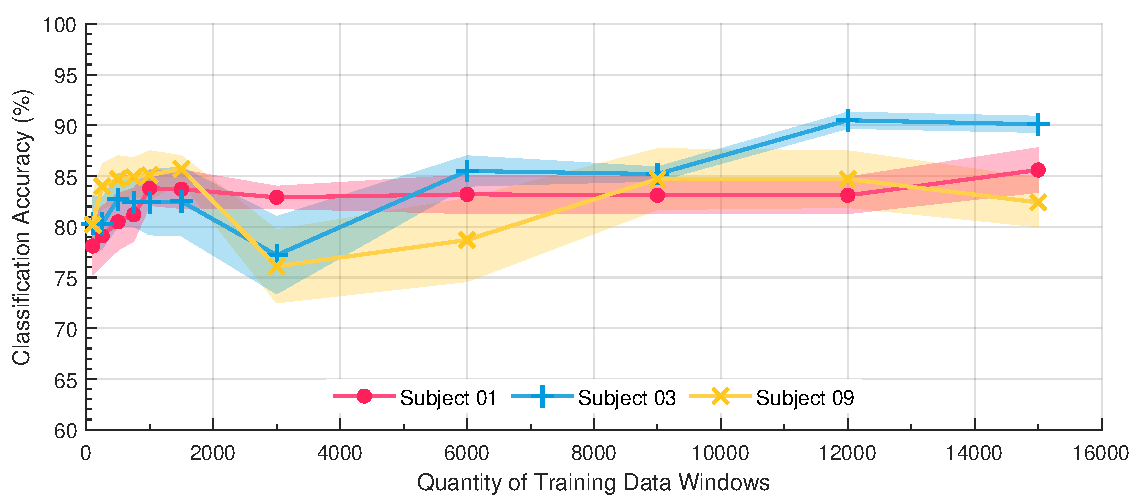
\includegraphics[width=\textwidth]{content/5-Personalisation/ch5_pre_trained_model_accuracy.pdf}
        \caption{Fine-tuning all layers}
        \label{subfig:ch5_fine-tuning-all-layers}
    \end{subfigure}
    \begin{subfigure}{\textwidth}
        \centering
        \includegraphics[width=\textwidth]{content/5-Personalisation/ch5_frozen_lstm_layer_accuracy.pdf}
        \caption{Fine-tuning only the dense layer}
    \end{subfigure}
    \caption[Results of fine-tuning a generic 32 unit \glsentryshort{lstm} model using increasing amounts of target data]{Results of fine-tuning a generic 32 unit \acrshort{lstm} model using increasing amounts of target data. The solid line represents the mean classification performance for each amount of training windows. The filled area represents the standard deviation $(n=25)$. Each of the 3 target subjects is represented individually. The red dot line is Subject 1, blue plus is subject 3 and yellow cross is subject 9.}
    \label{fig:ch5_pretrained_model}
\end{figure}
\begin{figure}[t]\ContinuedFloat
    \begin{subfigure}{\textwidth}
        \centering
        \includegraphics[width=\textwidth]{content/5-Personalisation/ch5_frozen_dense_layer_accuracy.pdf}
        \caption{Fine-tuning only the \acrshort{lstm} layer}
    \end{subfigure}
    \caption[]{Results of fine-tuning a generic 32 unit \acrshort{lstm} model using increasing amounts of target data (Cont.).}
\end{figure}

Figure \ref{subfig:ch5_fine-tuning-all-layers} shows the classification performance for fine-tuning all layers. The highest classification accuracy observed for each subject was $85.6\%$, $90.5\%$ and $84.7\%$ for subjects 1, 3 and 9 respectively. These were results were all achieved with either 12000 or 15000 target training windows. All models completed training in a small number of epochs, on average 5 with a 95\textsuperscript{th} percentile of 8.

Classification performance improves rapidly up to 1500 target training windows. When performance for 100, 250 and 500 training windows is compared to the bespoke baseline model performance is over 10\% better for all subjects. This potentially means only 30 seconds of each class are required. Performance improvements then increase more slowly with additional target data. The improvement over the bespoke model baseline also narrows to only a couple of percent.

Target windows quantities of 100-200 for subject 3 are also below the baseline performance. For subjects 3 and 9 performance drops down around 3000 target samples.  Other than these values all models exceed the baseline performance.

The drop in performance for higher values of training windows is still an improvement over the baselines for Subject 9 however briefly drops below the baseline general model for Subject 3. It's not obvious why this decrease in performance occurs but could be due to the introduction of a significantly different previously unseen environment to the training set.

Fine-tuning only the dense layer improved performance of Subject 3, no improvement for 9 and reduction in performance for 1. Standard deviation in general increased for all three subjects showing greater variation in performance across all models. When the dense layer was frozen there was a small improvement for subject 1 of greater than $1\%$ across all target window quantities but no meaningful change for subjects 3, and 9. Standard deviation remained largely the same when compared to fine-tuning all layers.

This approach to personalisation appears to give significant improvements in performance using only a small amount of target data. Only fine-tuning some layers doesn't give any consistent or meaningful improvement in performance.

%-------------------------------------------------------------------------------
\section{Discussion}
\label{sec:personalisation-discussion}
%What were we trying to achieve and have we achieved it?
The aim of these methods was to improve the performance of a \acrshort{lmr} network in both computation efficiency and classifier accuracy. 

Realistic testing scheme for personalisation methods?



%Do any of the methods show promise? Which model performed best
Both methods produced an improvement in accuracy, depending on the quantity of target data varied from greater than $10\%$ to just over $2\%$. However the data supplementation method required a significantly greater number of epochs to complete training.

Reduce data requirements for a new subject - yep
Reduce training requirements - using transfer learning yep

All of the methods showed a substantial performance improvements over the general model

All methods improved performance over the baseline model for the same quantity of target training samples

Data supplementation worked but it's difficult to predict how much additional data to add so would be difficult to implement in practice

For subjects 1 and 9 transfer learning is a better approach for subject 3 it's less obvious.



% How much data is required - results indicate you can never have enough. All models continued to improve with more data. Baseline, Supplementation and data grouping. All trained models gave the fastest early on, but although rate of improvement slowed down with increasing data it was still increasing.
More data would have improved things further. Not realistic to expose the model to every possible environment that it will need to operate on.
More data is always better - there no obvious point at which to stop so this work doesn't determine how much data is required



% Data grouping might be improved by being more selective over which subjects are included. Literature supports this. Area for further work
Mixed source and target data achieved better than transfer learning for lower amounts of target data windows. No predictable pattern to better classifications. Cost of substantially higher training epochs with more data so much slower.

Data supplementation technique is imprecise - it improves performance but more precision in the selection of supplemental data would probably improve things further 

With more selective source subjects this would probably have worked better. Additional measures would be needed to evaluate similarity between subjects, these are not needed when using purely deep learning approach.

Bias the data set towards the target data, using the general population to supplement the limited environments experienced by the subject. Similar to Balanced Batch Learning \cite{Cruciani2020}



% Negative transfer with addition target windows - why might that be. Introduction of new previously unseen environments. Because the data set of the target subjects was so large its likely that the subjects visited the same environments/areas multiple times.
Performance was better than baseline for the vast majority of tested configuration, just a couple of anomalies.

Interesting how performance degrades at different increasing amounts of data. Suspicion is that this is because of the introduction of new environments of data. Limited control on data collection demonstrates problems with real world data. Encountering a new environment or mislabelling of data can result in degraded performance. Would be interesting to investigate how introduction of new environments affect performance but a new/different data set collected in a controlled manner would be required for this.



% Transfer learning many other scheme that could have been attempted - trying adding adaption layers. Freezing of layers didn't really work - network might be too shallow. Different network architecture may lend themselves more to freezing specific layers.
Improved over the baseline - performance was more predictable although there was still inconsistencies due to the training data sets used. This was similar behaviour to the baseline model.

requires loading significantly less data into memory than data supplementation/grouping


This is a very simple configuration and transfer learning scheme but worked quite well. 

Not obvious if freezing layers helped likely just noise - more complex network architectures may have performed better here


% What are the limitations of this study/methods?
% Data limitations
Unable to tell what environments the data is collected in therefore can't really determine if a new environment causes the reduction in performance to occur. Could also be mislabelling.

Data is cleaned it up. Reduced transition data from data set, previous work indicated these were a large source in inaccuracy.

Data set didn't have enough control in it - could be useful to investigate what happens if a new environment is introduced


% Hyper-parameters limitation
Lots of room for hyper-parameter investigations - only loosely tuned


%Areas for further work
Could combine both methods - transfer learning with data grouping?

Now to apply to amputee data - this will be interesting as amputees have very different gait (asymmetric)


%-------------------------------------------------------------------------------
\section{Conclusions}
\label{sec:personalisation-conclusions}
The work in this chapter aimed to develop methods for personalisation of a \acrshort{lstm} \acrshort{lmr} network using a large source data set to supplement target data. These method will then be taken forward and applied to amputee data to try and reduce the data requirements.

Two methods were demonstrated, supplementing a target data to form an enlarged training set and fine-tuning a pre-trained general model. Both method were successful using the source data set to improve classification accuracy for the target users over the baseline. However the transfer learning approach achieved this performance in significantly fewer epochs requiring less computation resource. Therefore this is the method that will be taken forward.

After personalisation test subject 3 achieved a maximum classification accuracy of $90.5\%$ was achieved an improvement over $26.6\%$ over the baseline general model. The over two test subjects both achieved improvements of greater than $8.5\%$. When only a small amount of target training data is available, less than 30 seconds per activity class, performance of transfer learning is over 10\% better than training a model using only the target's data.

Following this study the methods developed will be tested using amputee data to see if these techniques can reduce the training data requirements for developing a classifier to improve the performance of a prosthetic limb.
\chapter{Applicability to Amputee Data}
\label{chp:amputee-data}

The collection of labelled training data is arduous; this problem becomes more acute when the subject has restricted movement, such as an amputee. Therefore, any system that can reduce these individuals' data requirements is of benefit. In Chapter \ref{chp:personalisation}, methods for personalisation of a machine learning model using additional data from other subjects were demonstrated to improve the model's performance and reduce the data requirements for that model. Within this Chapter, these methods will be implemented for an amputee to investigate if they apply to someone with an impaired gait.

The contributions of this Chapter are:
\begin{itemize}
    \item Collection of amputee gait data that is directly comparable to non-amputee data
    \item Comparison of shank \acrshort{marg} data between non-amputee, intact limb and prosthetic
    \item Demonstration of performance differences of \acrshort{lmr} network of intact and prosthetic side
    \item Demonstration of transfer learning from non-amputee data to an amputee for \acrshort{marg} gait data
\end{itemize}

First Section \ref{sec:amputee-methods} explains the methods used, and presents the collected amputee data. Following this in Sections \ref{sec:amputee-baseline}, \ref{sec:amputee-supplementation} and \ref{sec:amputee-transfer} present the results of a baseline model performance and performance of two personalisation methods, respectively. Finally, the discussion and conclusion are given in Section \ref{sec:amputee-discussion}.

From the literature the following gaps were identified:
\begin{itemize}
    \item No work has attempted to use transfer learning to personalise a non-amputee \acrshort{lmr} model for an amputee
    \item No papers have investigated the difference in classification performance between amputated and in-tact limb
\end{itemize}

The remainder of this Chapter will focus on investigating these gaps.

%-----------------------------------------------------------------
\section{Methods and Materials}
\label{sec:amputee-methods}
% Recap methods and what has changed
The methods used in this Chapter will mirror those used in previous chapters. Additional data for an amputee was collected. This was used to generate a new set of baselines to compare against and implement the previously developed personalisation methods. Complete tables of results for all experiments can be found in Appendix \ref{chp:tables-of-results} Section \ref{sec:app-a-amputee-transfer-learning}.

Data was collected from a single left trans-tibial amputee wearing a Blatchford Echelon VT prosthetic limb. Blatchford Product Limited collected the data. The data was collected in the same manner as previously described; however, a clinician at the centre held the smartphone to annotate activities to reduce the fall risk for the amputee. Data was collected walking around Blatchford's site in Basingstoke, both inside and outside. Table \ref{tab:summary-of-episode-amputee-data} summarises the data collected, including the number of data samples and the number of episodes for each activity.

\begin{table}[hbt]
    \centering
    \caption{Summary of amputee gait data collected}
    \label{tab:summary-of-episode-amputee-data}
    \begin{tabularx}{\textwidth}{c *{6}{Y}}
        \noalign{\hrule height 1.5pt}
        \textbf{Activity} & WALK  & \glsentryshort{ra} & \glsentryshort{rd} & \glsentryshort{sa} & \glsentryshort{sd} & STOP  \\
        \hline
        \textbf{Samples}  & 38114 & 6159               & 7194               & 2872               & 2450               & 11763 \\
        \textbf{Episodes} & 26    & 7                  & 7                  & 4                  & 4                  & 15    \\
        \noalign{\hrule height 1.5pt}                                                                                         \\
    \end{tabularx}
\end{table}

As significantly less data is available to test with, adjustments had to be made to the quantities used in each data set. The test data set was reduced from 5000 windows to 250 windows. The range of training windows tested was reduced to between 100 and 750. Additionally, to ensure that there were sufficient episodes for \acrshort{sa} and \acrshort{sd}, each of the stair episodes was split up into new episodes containing a maximum of 200 samples each. This increased the amount of available episodes for both stair activities.

Due to asymmetry, the left and right ankle data cannot be combined. This will be described further in the following section. All other quantities and hyper-parameters remained the same.

\subsection{Amputee Gait Data}
Gait asymmetry of amputees means that, unlike in the previous Chapter, the left and right ankle data cannot be combined to increase the dataset size. Instead, both sides will be evaluated independently to investigate the performance differences between the side. Figure \ref{fig:ch6_amputee_gyro_trends} shows the angular velocity of the shank in the sagittal plane for the intact and prosthetic limbs of a left amputated trans-tibial amputee. The left ankle has been transformed, so both ankles are presented in the same axes. For comparison, the ankle angular velocity of the non-amputee subject one is shown.

% How does it differ from non-amputee gait data
\begin{figure}[p]
    \begin{tabular}{lccc}
                                                                                                                                                 & \textbf{Non-Amputee}                                                                                                                  & \textbf{Amputee -- Prosthetic} & \textbf{Amputee -- Intact Limb} \vspace{0.2cm} \\

        \rotatebox{90}{\enspace\qquad \textbf{Walking}}                                                                                          &
        \begin{subfigure}[b]{0.275\textwidth}\includegraphics[width=\linewidth]{content/6-Amputee/Gait-Trends/ch6_subject_01_gait_trends_r_ankle_gyro_z_activity_walking.pdf}\end{subfigure}                                                                                                                & \begin{subfigure}[b]{0.275\textwidth}\includegraphics[width=\linewidth]{content/6-Amputee/Gait-Trends/ch6_amputee_gait_trends_l_ankle_gyro_z_activity_walking.pdf}\end{subfigure}                                                                                                             &
        \begin{subfigure}[b]{0.275\textwidth}\includegraphics[width=\linewidth]{content/6-Amputee/Gait-Trends/ch6_amputee_gait_trends_r_ankle_gyro_z_activity_walking.pdf}\end{subfigure}                                                                                                                                                                                                                                                                                                                                          \\

        \rotatebox{90}{~\quad \textbf{Ramp Ascent}}                                                                                              &
        \includegraphics[width=0.275\linewidth]{content/6-Amputee/Gait-Trends/ch6_subject_01_gait_trends_r_ankle_gyro_z_activity_ramp_up.pdf}    & \includegraphics[width=0.275\linewidth]{content/6-Amputee/Gait-Trends/ch6_amputee_gait_trends_l_ankle_gyro_z_activity_ramp_up.pdf}    &
        \includegraphics[width=0.275\linewidth]{content/6-Amputee/Gait-Trends/ch6_amputee_gait_trends_r_ankle_gyro_z_activity_ramp_up.pdf}                                                                                                                                                                                                                                 \\

        \rotatebox{90}{\quad \textbf{Ramp Descent}}                                                                                              &
        \includegraphics[width=0.275\linewidth]{content/6-Amputee/Gait-Trends/ch6_subject_01_gait_trends_r_ankle_gyro_z_activity_ramp_down.pdf}  & \includegraphics[width=0.275\linewidth]{content/6-Amputee/Gait-Trends/ch6_amputee_gait_trends_l_ankle_gyro_z_activity_ramp_down.pdf}  &
        \includegraphics[width=0.275\linewidth]{content/6-Amputee/Gait-Trends/ch6_amputee_gait_trends_r_ankle_gyro_z_activity_ramp_down.pdf}                                                                                                                                                                                                                               \\

        \rotatebox{90}{~\quad \textbf{Stair Ascent}}                                                                                             &
        \includegraphics[width=0.275\linewidth]{content/6-Amputee/Gait-Trends/ch6_subject_01_gait_trends_r_ankle_gyro_z_activity_stair_up.pdf}   & \includegraphics[width=0.275\linewidth]{content/6-Amputee/Gait-Trends/ch6_amputee_gait_trends_l_ankle_gyro_z_activity_stair_up.pdf}   &
        \includegraphics[width=0.275\linewidth]{content/6-Amputee/Gait-Trends/ch6_amputee_gait_trends_r_ankle_gyro_z_activity_stair_up.pdf}                                                                                                                                                                                                                                \\

        \rotatebox{90}{\quad \textbf{Stair Descent}}                                                                                             &
        \includegraphics[width=0.275\linewidth]{content/6-Amputee/Gait-Trends/ch6_subject_01_gait_trends_r_ankle_gyro_z_activity_stair_down.pdf} & \includegraphics[width=0.275\linewidth]{content/6-Amputee/Gait-Trends/ch6_amputee_gait_trends_l_ankle_gyro_z_activity_stair_down.pdf} &
        \includegraphics[width=0.275\linewidth]{content/6-Amputee/Gait-Trends/ch6_amputee_gait_trends_r_ankle_gyro_z_activity_stair_down.pdf}                                                                                                                                                                                                                              \\
    \end{tabular}
    \centering
    % \hspace*{1cm}\includegraphics[width=0.7\textwidth]{content/6-Amputee/Gait-Trends/Legend.pdf}
    \caption[Amputee and non-amputee shank angular velocity for different activities]{Angular velocity of the shank during different activities for an amputee and non-amputee. Data is for the sagittal Plane. The yellow line is for Non-Amputee (Subject 01 Left Ankle); The red line is the intact limb of the trans-tibial amputee; The blue line is the prosthetic of the trans-tibial amputee. The solid line shows the mean of the steps recorded for each activity. The filled area represents the standard deviation.}
    \label{fig:ch6_amputee_gyro_trends}
\end{figure}

From a visual assessment of the plots, differences between the non-amputee, intact and amputated limbs can be seen. The prosthetic limb shows significant differences to both the intact and non-amputee. The non-amputee and intact limb are closer in appearance.

Differences in the prosthetic limb are especially prevalent during heel strikes (at approximately 20\% of the gait cycle), where a much lower angular velocity is observed. In general, a more significant standard deviation is also seen for the prosthetic limb, suggesting more variation in the gait between steps.

This analysis covers one axis of the gyroscope. The visible differences can also be seen in the other two gyroscope axes and accelerometer signals. As the intact limb is closer to the non-amputee, it should be expected that it will perform more highly than the prosthetic side.

%-----------------------------------------------------------------
\section{Baseline Model Performance}
\label{sec:amputee-baseline}
As before, a set of baselines are needed to determine if the personalisation methods result in a performance improvement. All baselines will be evaluated using the amputee test data sets. The two baselines will be the performance of the general models and the performance of models constructed from only the target amputee's data.

The general models were constructed in the previous Chapter from the large source data set of gait data, excluding subjects 1, 3 and 9. These are all 32 unit \acrshort{lstm} models. Both the trans-tibial amputee's right intact limb and left prosthetic limb were tested separately. The general models achieved a classification performance of $74.2\%\pm9.4$ for the intact limb. For the amputated limb, the performance was significantly lower at $55.3\%\pm9.6$. From the previous study non-amputee subjects achieved around $72\%$, this is comparably to the performance of the intact limb.

Table \ref{tab:ch6-general-model-confusion-matrix} shows the confusion matrix for the general model. The matrix shows that the general mode performs poorly on walking and stair descent for both limbs. The performance for stair descent of the prosthetic limb is notable poor.

\begin{table}[!hbt]
    \centering
    \caption[Confusion matrix of general models presented with target subject test data]{Confusion matrix of general models presented with target subject test data. Columns represent the prediction labels, and the rows represent the actual labels. Each value represents the percentage of total predicted labels for that class. (\acrfull{ra}, \acrfull{rd}, \acrfull{sa}, \acrfull{sd})}
    \label{tab:ch6-general-model-confusion-matrix}
    \begin{subtable}{\textwidth}
        \caption{Prosthetic Limb}
        \begin{tabularx}{\textwidth}{ccYYYYYY}
            \noalign{\hrule height 1.5pt}
             &                    & \multicolumn{6}{c}{\textbf{Predicted Classes}}                                                                                            \\
            \hline
             &                    & WALK                                           & \glsentryshort{ra} & \glsentryshort{rd} & \glsentryshort{sa} & \glsentryshort{sd} & STOP \\
            \multirow{6}{*}{\rotatebox{90}{\textbf{True Classes}}}
             & WALK               & 46.6                                           & 12.8               & 9.0                & 1.7                & 23.1               & 5.9  \\
             & \glsentryshort{ra} & 8.5                                            & 77.7               & 0.0                & 9.8                & 13.4               & 10.6 \\
             & \glsentryshort{rd} & 26.0                                           & 6.4                & 91.0               & 0.3                & 33.7               & 2.1  \\
             & \glsentryshort{sa} & 0.0                                            & 0.4                & 0.0                & 88.1               & 0.0                & 1.0  \\
             & \glsentryshort{sd} & 14.5                                           & 2.6                & 0.0                & 0.1                & 29.3               & 18.0 \\
             & STOP               & 4.4                                            & 0.0                & 0.0                & 0.0                & 0.6                & 62.4 \\
            \noalign{\hrule height 1.5pt}
        \end{tabularx}
    \end{subtable}
    \begin{subtable}{\textwidth}
        \caption{Intact Limb}
        \begin{tabularx}{\textwidth}{ccYYYYYY}
            \noalign{\hrule height 1.5pt}
             &                    & \multicolumn{6}{c}{\textbf{Predicted Classes}}                                                                                            \\
            \hline
             &                    & WALK                                           & \glsentryshort{ra} & \glsentryshort{rd} & \glsentryshort{sa} & \glsentryshort{sd} & STOP \\
            \multirow{6}{*}{\rotatebox{90}{\textbf{True Classes}}}
             & WALK               & 69.8                                           & 0.6                & 11.6               & 0.2                & 14.9               & 0.4  \\
             & \glsentryshort{ra} & 14.3                                           & 97.5               & 0.0                & 21.7               & 7.8                & 4.4  \\
             & \glsentryshort{rd} & 8.5                                            & 0.0                & 73.4               & 0.0                & 20.7               & 0.0  \\
             & \glsentryshort{sa} & 0.0                                            & 0.0                & 0.0                & 77.7               & 0.0                & 0.0  \\
             & \glsentryshort{sd} & 0.1                                            & 1.9                & 15.0               & 0.1                & 55.5               & 0.8  \\
             & STOP               & 7.3                                            & 0.0                & 0.0                & 0.2                & 1.1                & 94.4 \\
            \noalign{\hrule height 1.5pt}
        \end{tabularx}
    \end{subtable}
\end{table}


%------------------------
The second baseline is a set of models trained using only the amputee data. Different quantities of training windows were used to provide performance metrics for various data amounts. Figure \ref{fig:ch6-amputee-baseline-bespoke-model} shows the classification performance for both legs when tested with the test data sets. The full results of this experiment can be found in  Appendix \ref{chp:tables-of-results} Table \ref{tab:amputee-bespoke-model-table-of-results}.  The average number of epochs to train for all models was 7, with a 95\textsuperscript{th} percentile of 9.

Figure \ref{fig:ch6-amputee-baseline-bespoke-model} shows performance improving rapidly with increasing training windows levelling out after 500 samples. In all cases the prosthetic limb performs worse than the intact limb. With increasing windows the performance gap stays consistent.

Table \ref{tab:ch6-bespoke-model-confusion-matrix} shows the confusion matrix for both limbs when a bespoke model was trained with 750 training windows. This is markedly better than the confusion matrix for the general model. This backs up the observations found in the literature that general models from non-amputees perform poorly for amputees\cite{Lonini2016, Jamieson2021}. However, several classes across both limbs perform worse than the general model, suggesting the general model contains knowledge that could be used to improve performance.

\begin{table}[!hbt]
    \centering
    \caption[confusion matrix for a bespoke amputee \acrshort{lmr} model presented test data]{confusion matrix for a bespoke amputee \acrshort{lmr} model presented with test data. The 32 unit \acrshort{lstm} model was trained with 750 target data window. Columns represent the prediction labels and the rows represent the real labels. Each value represent the percentage of total predicted labels for that class. (\acrfull{ra}, \acrfull{rd}, \acrfull{sa}, \acrfull{sd})}
    \label{tab:ch6-bespoke-model-confusion-matrix}
    \begin{subtable}{\textwidth}
        \caption{Prosthetic Limb}
        \begin{tabularx}{\textwidth}{ccYYYYYY}
            \noalign{\hrule height 1.5pt}
             &                    & \multicolumn{6}{c}{\textbf{Predicted Classes}}                                                                                             \\
            \hline
             &                    & WALK                                           & \glsentryshort{ra} & \glsentryshort{rd} & \glsentryshort{sa} & \glsentryshort{sd} & STOP  \\
            \multirow{6}{*}{\rotatebox{90}{\textbf{True Classes}}}
             & WALK               & 68.2                                           & 0.6                & 42.6               & 0.6                & 0.0                & 0.0   \\
             & \glsentryshort{ra} & 9.7                                            & 94.0               & 3.8                & 1.4                & 0.5                & 0.0   \\
             & \glsentryshort{rd} & 18.9                                           & 0.4                & 53.6               & 0.2                & 0.0                & 0.0   \\
             & \glsentryshort{sa} & 0.0                                            & 0.0                & 0.0                & 79.4               & 0.0                & 0.0   \\
             & \glsentryshort{sd} & 0.0                                            & 0.0                & 0.0                & 0.0                & 99.5               & 0.0   \\
             & STOP               & 3.2                                            & 4.9                & 0.0                & 18.4               & 0.0                & 100.0 \\
            \noalign{\hrule height 1.5pt}
        \end{tabularx}
    \end{subtable}
    % \end{table}
    % \begin{table}[t]\ContinuedFloat
    %  \caption[]{confusion matrix for a bespoke amputee \acrshort{lmr} model presented with test data. The 32 unit \acrshort{lstm} model was trained with 750 target data window (Cont.).}
    \begin{subtable}{\textwidth}
        \caption{Intact Limb}
        \begin{tabularx}{\textwidth}{ccYYYYYY}
            \noalign{\hrule height 1.5pt}
             &                    & \multicolumn{6}{c}{\textbf{Predicted Classes}}                                                                                            \\
            \hline
             &                    & WALK                                           & \glsentryshort{ra} & \glsentryshort{rd} & \glsentryshort{sa} & \glsentryshort{sd} & STOP \\
            \multirow{6}{*}{\rotatebox{90}{\textbf{True Classes}}}
             & WALK               & 83.1                                           & 2.6                & 19.3               & 0.0                & 0.0                & 0.0  \\
             & \glsentryshort{ra} & 12.3                                           & 93.3               & 7.4                & 12.0               & 0.0                & 0.8  \\
             & \glsentryshort{rd} & 3.7                                            & 0.0                & 72.0               & 0.1                & 3.3                & 0.0  \\
             & \glsentryshort{sa} & 0.0                                            & 0.0                & 0.0                & 83.6               & 0.0                & 0.0  \\
             & \glsentryshort{sd} & 0.0                                            & 0.0                & 0.0                & 0.0                & 96.7               & 0.0  \\
             & STOP               & 0.9                                            & 4.1                & 1.2                & 4.3                & 0.0                & 99.2 \\
            \noalign{\hrule height 1.5pt}
        \end{tabularx}
    \end{subtable}
\end{table}

\begin{figure}[H]
    \centering
    \includegraphics[width=\textwidth]{content/6-Amputee/ch6_baseline_model_accuracy.pdf}
    \caption[Classification accuracy using increasing quantities of amputee target data]{Classification accuracy for HAR model using increasing quantities of only amputee target data. The red line shows the performance of the trained model on the intact limb of a trans-tibial amputee. The blue line shows the performance of the trained model for the prosthetic side. The filled areas represent the standard deviation (n=20).}
    \label{fig:ch6-amputee-baseline-bespoke-model}
\end{figure}


%-----------------------------------------------------------------
\section{Data supplementation} % Are we going to include this?
\label{sec:amputee-supplementation}
The first personalised model technique that will be investigated is data supplementation. This involves supplementing target data with a varying amount of data from a general source set to form a large training set. The source data is made up of a larger number of non-amputee subjects.

The experiment consisted of mixing 100, 250, 500 and 750 target data windows with between 100 and 3000 source windows. On average, each model took 10 epochs to train, 95\textsuperscript{th} percentile of 17. In general, the more data used, the larger the number of epochs required. Table \ref{tab:ch6-classfication-accuracy-mixed-source-target-right} shows classification performance for all combinations.

As before, the performance of the prosthetic side is lower than the intact side. All classification accuracies for the prosthetic exceed the general model performance. However, the lowest two results for 100 source windows perform worse than the general model for the intact limb.

For the intact side, none of the 500 and 750 target window models exceeds the performance of the bespoke models with the same quantity of target windows. For the amputated side, all but 750 target window, 100 source window result exceed the bespoke model performance.

At a lower value of target windows, a higher quantity of source windows improves performance; less source data is needed at higher target windows. At higher values of target data windows, the performance improvement is minimal, especially for the intact side. This suggests that this method may become less valuable the more target data available.

\begin{table}[!hbt]
    \caption[Table of classification accuracy for amputee test data for a model trained using varying amounts of Source and Target training data]{Table of classification accuracy for amputee test data for a model trained using varying amounts of Source and Target training data. The cell value represents the percentage classification accuracy $\pm\sigma$ $(n=8)$. The highest classification accuracy for each quantity of target windows has been highlighted in bold}
    \label{tab:ch6-classfication-accuracy-mixed-source-target-right}
    \centering
    \begin{subtable}{\textwidth}
        \centering
        \caption{Intact Limb} % Right
        \begin{tabularx}{0.99\textwidth}{cr| *{4}{Y}}
            \noalign{\hrule height 1.5pt}
             &      & \multicolumn{4}{c}{\textbf{Target Training Windows}}                                                                                                                                           \\
             &      & 100                                                  & 250                                         & 500                                         & 750                                         \\
            \hline
            \multirow{7}{*}{\rotatebox{90}{\parbox{3.4cm}{\centering\textbf{Source Training                                                                                                                          \\Windows}}}}
             & 0    & $0.428{\scriptscriptstyle\pm0.05}$                   & $0.448{\scriptscriptstyle\pm0.05}$          & $0.863{\scriptscriptstyle\pm0.02}$          & $0.869{\scriptscriptstyle\pm0.01}$          \\
             & 100  & $0.717{\scriptscriptstyle\pm0.03}$                   & $0.682{\scriptscriptstyle\pm0.02}$          & $0.879{\scriptscriptstyle\pm0.02}$          & $0.877{\scriptscriptstyle\pm0.04}$          \\
             & 250  & $0.764{\scriptscriptstyle\pm0.04}$                   & $0.730{\scriptscriptstyle\pm0.03}$          & $0.883{\scriptscriptstyle\pm0.03}$          & $\mathbf{0.889{\scriptscriptstyle\pm0.01}}$ \\
             & 500  & $0.800{\scriptscriptstyle\pm0.04}$                   & $0.795{\scriptscriptstyle\pm0.03}$          & $0.875{\scriptscriptstyle\pm0.02}$          & $0.888{\scriptscriptstyle\pm0.02}$          \\
             & 750  & $0.815{\scriptscriptstyle\pm0.01}$                   & $0.801{\scriptscriptstyle\pm0.02}$          & $0.873{\scriptscriptstyle\pm0.02}$          & $0.881{\scriptscriptstyle\pm0.02}$          \\
             & 1000 & $0.801{\scriptscriptstyle\pm0.04}$                   & $0.786{\scriptscriptstyle\pm0.03}$          & $\mathbf{0.886{\scriptscriptstyle\pm0.03}}$ & $0.874{\scriptscriptstyle\pm0.02}$          \\
             & 1500 & $\mathbf{0.835{\scriptscriptstyle\pm0.03}}$          & $0.794{\scriptscriptstyle\pm0.06}$          & $0.871{\scriptscriptstyle\pm0.01}$          & $0.875{\scriptscriptstyle\pm0.03}$          \\
             & 3000 & $0.825{\scriptscriptstyle\pm0.01}$                   & $\mathbf{0.826{\scriptscriptstyle\pm0.07}}$ & $0.846{\scriptscriptstyle\pm0.03}$          & $0.863{\scriptscriptstyle\pm0.03}$          \\
            \noalign{\hrule height 1.5pt}                                                                                                                                                                            \\
        \end{tabularx}
    \end{subtable}

    \begin{subtable}{\textwidth}
        \centering
        \caption{Prosthetic Limb} % Left
        \begin{tabularx}{0.99\textwidth}{cr| *{4}{Y}}
            \noalign{\hrule height 1.5pt}
             &      & \multicolumn{4}{c}{\textbf{Target Training Windows}}                                                                                                                                           \\
             &      & 100                                                  & 250                                         & 500                                         & 750                                         \\
            \hline
            \multirow{7}{*}{\rotatebox{90}{\parbox{3.4cm}{\centering\textbf{Source Training                                                                                                                          \\Windows}}}}
             & 0    & $0.447{\scriptscriptstyle\pm0.02}$                   & $0.469{\scriptscriptstyle\pm0.03}$          & $0.765{\scriptscriptstyle\pm0.04}$          & $0.830{\scriptscriptstyle\pm0.03}$          \\
             & 100  & $0.626{\scriptscriptstyle\pm0.05}$                   & $0.643{\scriptscriptstyle\pm0.03}$          & $0.855{\scriptscriptstyle\pm0.02}$          & $0.813{\scriptscriptstyle\pm0.04}$          \\
             & 250  & $0.714{\scriptscriptstyle\pm0.04}$                   & $0.611{\scriptscriptstyle\pm0.02}$          & $0.836{\scriptscriptstyle\pm0.05}$          & $0.843{\scriptscriptstyle\pm0.03}$          \\
             & 500  & $0.752{\scriptscriptstyle\pm0.03}$                   & $0.729{\scriptscriptstyle\pm0.08}$          & $0.842{\scriptscriptstyle\pm0.02}$          & $0.840{\scriptscriptstyle\pm0.05}$          \\
             & 750  & $0.734{\scriptscriptstyle\pm0.06}$                   & $0.712{\scriptscriptstyle\pm0.04}$          & $0.848{\scriptscriptstyle\pm0.03}$          & $0.847{\scriptscriptstyle\pm0.02}$          \\
             & 1000 & $0.756{\scriptscriptstyle\pm0.02}$                   & $0.756{\scriptscriptstyle\pm0.08}$          & $\mathbf{0.875{\scriptscriptstyle\pm0.03}}$ & $\mathbf{0.872{\scriptscriptstyle\pm0.01}}$ \\
             & 1500 & $0.734{\scriptscriptstyle\pm0.02}$                   & $\mathbf{0.764{\scriptscriptstyle\pm0.05}}$ & $0.869{\scriptscriptstyle\pm0.02}$          & $0.852{\scriptscriptstyle\pm0.02}$          \\
             & 3000 & $\mathbf{0.767{\scriptscriptstyle\pm0.02}}$          & $\mathbf{0.764{\scriptscriptstyle\pm0.04}}$ & $0.874{\scriptscriptstyle\pm0.02}$          & $0.849{\scriptscriptstyle\pm0.02}$          \\
            \noalign{\hrule height 1.5pt}                                                                                                                                                                            \\
        \end{tabularx}
    \end{subtable}
\end{table}



%-----------------------------------------------------------------
\section{Transfer Learning}
\label{sec:amputee-transfer}
Transfer learning involves using the knowledge captured in an existing model as a starting point to building a personalised model. For this experiment, five general models constructed in Chapter \ref{chp:personalisation} were used as the starting point. Varying quantities of target amputee data windows were then used to fine-tune these starting models to personalise them to the amputee. By freezing the different network layers, attempts to reduce the computation load required to train the model could be made.

Figure \ref{fig:ch6-amputee-retrain-pre-trained} shows three different experiments in transfer learning. Each trained different layers of the network. The first trained all layers, the second just the dense layer, and finally just the \acrshort{lstm} layer.

\begin{figure}[!hbtp]
    \centering
    \begin{subfigure}{\textwidth}
        \centering
        \includegraphics[width=\textwidth]{content/6-Amputee/ch6_pre_trained_model_accuracy.pdf}
        \caption{Fine tuning all layers}
    \end{subfigure}
    \begin{subfigure}{\textwidth}
        \centering
        \includegraphics[width=\textwidth]{content/6-Amputee/ch6_frozen_lstm_layer_accuracy.pdf}
        \caption{Fine tuning only the dense layer}
    \end{subfigure}
    \caption[Accuracy of re-training a pre-trained model using amputee target data]{Classification accuracy for re-training a pre-trained model using increasing quantities of amputee target data. The red line shows the performance of the trained model on the intact limb of a trans-tibial amputee. The blue line shows the performance of the trained model for the prosthetic side. The filled areas represent the standard deviation (n=20).}
    \label{fig:ch6-amputee-retrain-pre-trained}
\end{figure}
\begin{figure}[t]\ContinuedFloat
    \centering
    \begin{subfigure}{\textwidth}
        \includegraphics[width=\textwidth]{content/6-Amputee/ch6_frozen_dense_layer_accuracy.pdf}
        \caption{Fine tuning only the \acrshort{lstm} layer}
    \end{subfigure}
    \caption[]{Classification accuracy for re-training a pre-trained model using increasing quantities of amputee target data (Cont.).}
\end{figure}

On average, each model took 6 epochs 95\textsuperscript{th} percentile of 10. In general, the more data used, the larger the number of epochs required.

When training all layers, classification performance significantly increased over the base general model with only a few target windows. For the prosthetic side with 100 target windows, there was a $22\%$ increase in performance over the general model. This reduced to just under $1\%$ for the intact limb at 750 windows. The improvement over the bespoke model slightly higher achieving at least a $3\%$ improvement. Overall transfer learning resulted in an improvement for all configurations.

Fine-tuning only the dense layer did not result in better performance than fine-tuning all layers and for the intact limb at 500 and 750 windows was worse than the baseline bespoke model. Using this method significantly increased standard deviation for the prosthetic limb, although slightly reduced $\sigma$ for the intact limb.

Fine-tuning only the \acrshort{lstm} layer gave the best performance for 100 and 250 target windows compared to fine-tuning all layers. Performance was a couple of percent better; however, the higher two target window quantities performance was approximately a percent worse. The standard deviation remained roughly the same. On balance, it showed no improvement over fine-tuning all layers.

%-----------------------------------------------------------------
\section{Discussion and Conclusions}
\label{sec:amputee-discussion}
The work in this Chapter set out to investigate if the personalisation methods for an \acrshort{lmr} classifier developed in Chapter \ref{chp:personalisation} were applicable to an amputee. A set of comparable data was collected from a trans-tibial amputee to achieve this. This was then used to repeat the previous experiments for the amputee subject.

Jamieson and Lonini suggested that the direct use of a general model trained using only non-amputee data would not perform adequately for a person with gait impairments\cite{Lonini2016, Jamieson2021}. This was borne out in the results when data from the prosthetic limb was tested. It achieved a classification accuracy of $55.3\%$, significantly less than the non-amputee subjects.

When data from the amputee's intact limb was used, classification performance was much higher. The test subject has a significant asymmetry in their gait, with the intact side matching more closely to the source non-amputees gait. This is an area that requires additional research as it is potentially an easy way to improve the performance of an amputee gait classifier.

Both the data supplementation and transfer learning approaches improved over the baseline classifiers. The differences observed in the previous Chapter were again shown. The quantity of source data required for data supplementation was hard to predict, and only training specific layers for transfer learning resulted in minimal changes. As before, the transfer learning performance appeared to perform more consistently and required significantly less computing resources to train.

The overall performance of both the bespoke model and personalised models at 500 and 750 training windows was significantly higher than seen in the previous Chapter. They also looked more likely to be levelling off in performance. There are two likely reasons for this. First, a much smaller testing set was used, so the trained model was tested with a narrower range of environments. Secondly, all the amputee data was collected at a single site, and therefore the training data is likely to include environments seen in the test set. The division of stairs episodes would also have a similar effect.

Further, as data for only one amputee was collected, it is not possible to say whether these methods are more generally applicable. To test the results further, more amputees and more data per amputee are required.

In the previous Chapter, a method for improving data supplementation was data grouping. It is unlikely to be successful in this scenario due to the likely difficulty in finding subjects with a similar gait to an amputee. However, there may be potential in including more persons with gait impairments to improve the networks ability to adapt. This is a potential area for further research.

No literature was found investigating the classification performance difference between the two lower limbs of an amputee or other person with asymmetric gait. The results consistently showed that classification of the intact limb had higher accuracies than the amputated limb. This could be an exciting area of research for improving the classifier's performance using both sides of the body. A form of ensemble network could be a good candidate for this.

The personalisation approach shows promise in the area of amputee gait classification. As concluded in the previous chapter the general training population should ideally contain individuals of similar gait to the target subject. This is significantly harder for amputees. Further research is required in this area to exploit the potential for using non-amputee data to reduce data requirements for amputees and to investigate the limitations of this approach. Further research into the use of the intact limb to improve classification performance is also required,

\chapter{Conclusions and Further Work}
\label{chp:conclusions}
In this Chapter, the work conducted towards developing an \acrshort{ml} method for an activity classifier for an amputee to improve locomotion mode selection in the powered prosthesis is briefly discussed. This is followed by some suggestions for further work to continue this research.

\section{Conclusions} % Talk aims, implementation, achievements, limitations
An effort was made to contribute to the development of a locomotion mode classifier for amputees in the hope that this will be useful to the improvement of powered prosthetic devices. Specifically, the hypothesis stated in the Introductory Chapter was:

\textbf{A Machine Learning approach based on \acrfull{lstm} architecture can be used to predict gait modes with data requirements reduced through a transfer learning approach.}

A literature survey was conducted to establish the background around gait, lower limb powered prosthesis, and Machine Learning methods. The need for a system to identify an amputee's current locomotive intent to inform the selection of appropriate control modes was established. The current state of the art research has not demonstrated IMU-based ML classifiers applied to amputees; however, they have been applied to individuals without gait impairment. This appears to be partly due to the difficulties in collecting a large enough data set of amputee gait data. But also due to the highly individual nature of gait, especially for amputees. The need for further research in this area was established, especially for ways to reduce data requirements and increase performance.

In order to address these research gaps, a large set of gait data is required from non-amputees and amputees. As IMU gait data for lower limb amputees could not be found, a new data set is required. A novel system comprised of wireless IMUs and a companion smartphone app was developed to achieve this. This allowed for the unsupervised collection of labelled natural gait data from numerous individuals. Methods were developed for post-processing the gait data to prepare it for use in a TensorFlow ML environment. Work was also undertaken to develop the TensorFlow ML environment.

A journal article published in Sensors was presented that investigated the internal behaviour of an LSTM based LMR classifier. A public dataset of 22 individuals was collected using the previous Chapter's methodology. This data set was used to analyse the internal behaviour of a reduced complexity LSTM network. Experiments around analysing the network's hidden state were undertaken to establish a link between the input data and output classification. The analysis identifies that the model primarily classifies activity type based on data around early stance. Additional work was undertaken on a full LSTM LMR network to identify activity types for unseen novel subjects. Evaluation of generalisation for unseen subjects reveals low sensitivity to hyper-parameters with issues caused by over-fitting individuals' gait traits. Although an accuracy of greater than $95\%$ is possible for a seen individual classification, the network struggled to classify unseen individuals, achieving around $80\%$. Investigating the differences between individual subjects showed that gait variations between users primarily occur in early stance, potentially explaining the poor generalisation. Adjustment of hyper-parameters alone could not solve this, demonstrating the need for individual personalisation of models.

Based on the need for individual personalisation, methods for achieving this were investigated. A survey of literature revealed that transfer learning is a promising approach. However, its applicability to real-world data has not been investigated, nor has the requirements for the quantity of a target individual's data. Additional data for three subjects was collected using the previous methods developed. This allowed for an extensive study of the benefits of transfer learning with different quantities of target subject data. In order to use the unstructured real-world continuous data, new methods for data division were required. The data was poorly distributed, and therefore data rebalancing was required. This was accomplished by dividing the data into episodes, each containing a single continuous period of one activity. By combining episodes, a balanced data set could be constructed. This also had the benefit of allowing for multiple data sets to be systematically built and ensuring that the test data set was unseen.

A set of baselines were developed to compare the network's performance against. These were the best performance that could be achieved by either a general model built for other's data or a fully bespoke model constructed for a target subject's data. Two personalisation methods were attempted, data supplementation and transfer learning. Both methods improved the performance of the target subject's classification, achieving $90\%$ maximum. The maximum improvements were seen at low quantities of target data, demonstrating both methods showed promise for situations where only limited data is available.

Following the development of the personalisation methods, their applicability to amputees was evaluated. The literature found that studies had struggled to classify amputees using gait data from non-amputees. However, no study had attempted personalisation techniques using amputee data. There was also no investigation into differences in how the amputated and intact limbs would perform. Amputees have a very asymmetric gait; therefore, it should be expected that both legs would have different classification performances. A small set of amputee data was collected from a single trans-tibial amputee to investigate personalisation methods. Using the methodology previously discussed, personalisation experiments were repeated. The results showed a dramatic improvement in classification performance using limited amputee data. Both personalisation methods worked, achieving $90\%$ accuracy for the intact limb and just under $90\%$ for the amputated limb. Due to the limited data available for testing, it is not possible to say how generally these methods work, but they appear promising and should be investigated further.

This work has raised many additional research questions. Such as the applicable of the amputee personalisation result to people with other gait abnormalities. There is future research in to the use of an amputees intact limb classifier to improve gait classification. These form areas that could be focus of future research.

The work allows for large scale collection of gait data that is free from laboratory constraints while reducing gait bias from researchers. The work also highlighted the improvements in classification performance that can be achieved by using a general population as a starting point for building a bespoke classifier. Initial work indicates that this is highly applicable to classifying individual with gait abnormalities. Further work is still required to see how generally applicable this is to amputees and other gait abnormalities.

\section{Further Work} % One Step Beyond
The work conducted has demonstrated that this is an area of research with promise. However, there are numerous aspects where additional research could yield improvements. These include:

\begin{itemize}
    \item Additional amputees --  The trial only included a single trans-tibial amputee. Additional amputee trials should involve multiple subjects, including amputees of different weights, heights, and levels of amputation in multiple environments to test the applicability more generally.
    
    \item Investigate how the transition will affect performance -- Due to the data division scheme employed for the personality study, the transition between activities was not considered. In Chapter \ref{chp:lstm-general} transition was identified as a key area of error. Looking at how classification performance changes around this area would inform knowledge of the current performance of the model during transition. Changes to the labelling of transitions, \acrshort{ml} model architecture, and model hyper-parameters should then be investigated to see if transition performance can be improved.
    
    \item A greater number of environments -- It was hypothesised that the addition of new environments affects performance; however, due to the limited data labelling, it was not possible to investigate this. Modifying the app to store location data would allow for greater detail to be understood about the environment. By using map data the type of environment could be automatically tagged. Classification performance could then be filtered to see how performance changes based on different environments.
    
    \item Investigate more complex LMR networks -- A very shallow LSTM network was investigated. This was selected due to its adequate performance and ability to iterate quickly with a shallow network. Other work has successfully used deeper and more sophisticated networks; this should be explored further. There is also a large scope for hyper-parameter optimisation as only a little work was performed in this area.
    
    \item Implementation for real-time -- The fact that the system works on a smartphone means that a system could be deployed in the real world for more extensive testing. Direct real-time feedback on the models performance could be used to inform a semi-supervised learning system. This would allow for far greater data quantities to be used during training without the need for direct user labelling.
\end{itemize}




% -- Appendix --
\appendix % switch to appendix mode
\chapter{Tables of Results}
\label{chp:tables-of-results}
This Appendix contains tables of data for Chapter \ref{chp:personalisation} which investigated personalisation methods for LSTM models using data for non-amputees.

\section{Tables of Model Performance for Non-Amputee Bespoke Target Model}
\label{sec:appendix-a-model-performance-bespoke}
The following section contains tables of data for investigation into classification performance for LSTM models trained using increasing amounts of a target subject data. This section contains Tables \ref{tab:classifcation_performance_target_data_bespoke_subject_01}, \ref{tab:classifcation_performance_target_data_bespoke_subject_03} and \ref{tab:classifcation_performance_target_data_bespoke_subject_09}
\vfill
\  \\
\begin{table}[H]
    \centering
    \caption[Table of results for classification performance of different size \glsentryshort{lstm} networks trained with varying amount of target subject data for subject 1.]{Table of results for classification performance of different size \glsentryshort{lstm} networks trained with varying amount of target subject data for subject 1. The table shows the classification accuracy for the target user training, validation and test data sets $\pm\sigma(n = 25)$. A value of one represents 100\% correct classification.}
    \label{tab:classifcation_performance_target_data_bespoke_subject_01}
    \begin{tabularx}{\textwidth}{cc | YYYc | YYYc }
        \noalign{\hrule height 1.5pt}
        & & \multicolumn{4}{c|}{\textbf{6 Units}} & \multicolumn{4}{c}{\textbf{16 Units}} \\
        & & Train & Valid & Test & Epochs & Train & Valid & Test & Epochs \\
        \hline
        \multirow{11}{*}{\rotatebox{90}{\parbox{5.3cm}{\centering\textbf{Target Training Windows}}}}
        & 100 & $0.697{\scriptscriptstyle\pm0.10}$ & $0.477{\scriptscriptstyle\pm0.10}$ & $0.492{\scriptscriptstyle\pm0.07}$ & 36 & $0.776{\scriptscriptstyle\pm0.04}$ & $0.477{\scriptscriptstyle\pm0.04}$ & $0.527{\scriptscriptstyle\pm0.03}$ & 22 \\
        & 250 & $0.765{\scriptscriptstyle\pm0.08}$ & $0.543{\scriptscriptstyle\pm0.09}$ & $0.570{\scriptscriptstyle\pm0.10}$ & 22 & $0.805{\scriptscriptstyle\pm0.09}$ & $0.542{\scriptscriptstyle\pm0.07}$ & $0.607{\scriptscriptstyle\pm0.09}$ & 12 \\
        & 500 & $0.783{\scriptscriptstyle\pm0.09}$ & $0.599{\scriptscriptstyle\pm0.05}$ & $0.655{\scriptscriptstyle\pm0.09}$ & 12 & $0.875{\scriptscriptstyle\pm0.03}$ & $0.641{\scriptscriptstyle\pm0.03}$ & $0.743{\scriptscriptstyle\pm0.06}$ & 9 \\
        & 750 & $0.835{\scriptscriptstyle\pm0.04}$ & $0.623{\scriptscriptstyle\pm0.06}$ & $0.682{\scriptscriptstyle\pm0.06}$ & 10 & $0.899{\scriptscriptstyle\pm0.05}$ & $0.617{\scriptscriptstyle\pm0.03}$ & $0.726{\scriptscriptstyle\pm0.05}$ & 7 \\
        & 1000 & $0.821{\scriptscriptstyle\pm0.04}$ & $0.713{\scriptscriptstyle\pm0.04}$ & $0.736{\scriptscriptstyle\pm0.05}$ & 15 & $0.854{\scriptscriptstyle\pm0.02}$ & $0.704{\scriptscriptstyle\pm0.02}$ & $0.782{\scriptscriptstyle\pm0.04}$ & 8 \\
        & 1500 & $0.816{\scriptscriptstyle\pm0.02}$ & $0.713{\scriptscriptstyle\pm0.02}$ & $0.752{\scriptscriptstyle\pm0.05}$ & 17 & $0.864{\scriptscriptstyle\pm0.02}$ & $0.689{\scriptscriptstyle\pm0.02}$ & $0.752{\scriptscriptstyle\pm0.04}$ & 8 \\
        & 3000 & $0.823{\scriptscriptstyle\pm0.03}$ & $0.777{\scriptscriptstyle\pm0.04}$ & $0.753{\scriptscriptstyle\pm0.06}$ & 18 & $0.864{\scriptscriptstyle\pm0.03}$ & $0.763{\scriptscriptstyle\pm0.03}$ & $0.752{\scriptscriptstyle\pm0.05}$ & 11 \\
        & 6000 & $0.840{\scriptscriptstyle\pm0.03}$ & $0.771{\scriptscriptstyle\pm0.06}$ & $0.750{\scriptscriptstyle\pm0.06}$ & 24 & $0.909{\scriptscriptstyle\pm0.03}$ & $0.776{\scriptscriptstyle\pm0.04}$ & $0.789{\scriptscriptstyle\pm0.05}$ & 12 \\
        & 9000 & $0.848{\scriptscriptstyle\pm0.02}$ & $0.718{\scriptscriptstyle\pm0.03}$ & $0.741{\scriptscriptstyle\pm0.04}$ & 18 & $0.903{\scriptscriptstyle\pm0.02}$ & $0.732{\scriptscriptstyle\pm0.03}$ & $0.788{\scriptscriptstyle\pm0.05}$ & 11 \\
        & 12000 & $0.851{\scriptscriptstyle\pm0.03}$ & $0.738{\scriptscriptstyle\pm0.05}$ & $0.784{\scriptscriptstyle\pm0.05}$ & 23 & $0.907{\scriptscriptstyle\pm0.02}$ & $0.742{\scriptscriptstyle\pm0.03}$ & $0.814{\scriptscriptstyle\pm0.04}$ & 13 \\
        & 15000 & $0.813{\scriptscriptstyle\pm0.04}$ & $0.732{\scriptscriptstyle\pm0.06}$ & $0.783{\scriptscriptstyle\pm0.04}$ & 23 & $0.889{\scriptscriptstyle\pm0.02}$ & $0.764{\scriptscriptstyle\pm0.03}$ & $0.844{\scriptscriptstyle\pm0.03}$ & 15 \\
        \noalign{\hrule height 1.5pt} \\
    \end{tabularx}
    \begin{tabularx}{\textwidth}{cc | YYYc | YYYc }
        \noalign{\hrule height 1.5pt}
        & & \multicolumn{4}{c|}{\textbf{32 Units}} & \multicolumn{4}{c}{\textbf{64 Units}} \\
        & & Train & Valid & Test & Epochs & Train & Valid & Test & Epochs \\
        \hline
        \multirow{11}{*}{\rotatebox{90}{\parbox{5.3cm}{\centering\textbf{Target Training Windows}}}}
        & 100 & $0.801{\scriptscriptstyle\pm0.05}$ & $0.497{\scriptscriptstyle\pm0.05}$ & $0.566{\scriptscriptstyle\pm0.04}$ & 16 & $0.724{\scriptscriptstyle\pm0.09}$ & $0.439{\scriptscriptstyle\pm0.07}$ & $0.521{\scriptscriptstyle\pm0.08}$ & 9\\
        & 250 & $0.815{\scriptscriptstyle\pm0.08}$ & $0.531{\scriptscriptstyle\pm0.03}$ & $0.622{\scriptscriptstyle\pm0.05}$ & 8 & $0.869{\scriptscriptstyle\pm0.04}$ & $0.540{\scriptscriptstyle\pm0.03}$ & $0.650{\scriptscriptstyle\pm0.03}$ & 7\\
        & 500 & $0.883{\scriptscriptstyle\pm0.03}$ & $0.631{\scriptscriptstyle\pm0.03}$ & $0.720{\scriptscriptstyle\pm0.05}$ & 6 & $0.907{\scriptscriptstyle\pm0.03}$ & $0.615{\scriptscriptstyle\pm0.04}$ & $0.746{\scriptscriptstyle\pm0.03}$ & 5\\
        & 750 & $0.934{\scriptscriptstyle\pm0.02}$ & $0.633{\scriptscriptstyle\pm0.02}$ & $0.749{\scriptscriptstyle\pm0.03}$ & 5 & $0.932{\scriptscriptstyle\pm0.02}$ & $0.627{\scriptscriptstyle\pm0.02}$ & $0.727{\scriptscriptstyle\pm0.04}$ & 4\\
        & 1000 & $0.888{\scriptscriptstyle\pm0.02}$ & $0.696{\scriptscriptstyle\pm0.02}$ & $0.774{\scriptscriptstyle\pm0.04}$ & 7 & $0.886{\scriptscriptstyle\pm0.02}$ & $0.694{\scriptscriptstyle\pm0.02}$ & $0.765{\scriptscriptstyle\pm0.03}$ & 5\\
        & 1500 & $0.865{\scriptscriptstyle\pm0.01}$ & $0.704{\scriptscriptstyle\pm0.03}$ & $0.758{\scriptscriptstyle\pm0.04}$ & 6 & $0.885{\scriptscriptstyle\pm0.02}$ & $0.693{\scriptscriptstyle\pm0.02}$ & $0.771{\scriptscriptstyle\pm0.02}$ & 5\\
        & 3000 & $0.895{\scriptscriptstyle\pm0.04}$ & $0.752{\scriptscriptstyle\pm0.02}$ & $0.767{\scriptscriptstyle\pm0.02}$ & 8 & $0.921{\scriptscriptstyle\pm0.03}$ & $0.754{\scriptscriptstyle\pm0.02}$ & $0.771{\scriptscriptstyle\pm0.01}$ & 8\\
        & 6000 & $0.924{\scriptscriptstyle\pm0.03}$ & $0.758{\scriptscriptstyle\pm0.06}$ & $0.781{\scriptscriptstyle\pm0.06}$ & 10 & $0.937{\scriptscriptstyle\pm0.01}$ & $0.719{\scriptscriptstyle\pm0.03}$ & $0.776{\scriptscriptstyle\pm0.03}$ & 8\\
        & 9000 & $0.923{\scriptscriptstyle\pm0.03}$ & $0.710{\scriptscriptstyle\pm0.05}$ & $0.778{\scriptscriptstyle\pm0.05}$ & 9 & $0.917{\scriptscriptstyle\pm0.02}$ & $0.709{\scriptscriptstyle\pm0.03}$ & $0.752{\scriptscriptstyle\pm0.04}$ & 7\\
        & 12000 & $0.920{\scriptscriptstyle\pm0.04}$ & $0.712{\scriptscriptstyle\pm0.03}$ & $0.798{\scriptscriptstyle\pm0.01}$ & 10 & $0.902{\scriptscriptstyle\pm0.04}$ & $0.712{\scriptscriptstyle\pm0.04}$ & $0.779{\scriptscriptstyle\pm0.03}$ & 7\\
        & 15000 & $0.903{\scriptscriptstyle\pm0.02}$ & $0.780{\scriptscriptstyle\pm0.04}$ & $0.839{\scriptscriptstyle\pm0.03}$ & 17 & $0.889{\scriptscriptstyle\pm0.06}$ & $0.743{\scriptscriptstyle\pm0.06}$ & $0.805{\scriptscriptstyle\pm0.06}$ & 10\\
        \noalign{\hrule height 1.5pt} \\
    \end{tabularx}
\end{table}

\begin{table}[H]
    \centering
    \caption[Table of results for classification performance of different size \glsentryshort{lstm} networks trained with varying amount of target subject data for subject 3.]{Table of results for classification performance of different size \glsentryshort{lstm} networks trained with varying amount of target subject data for subject 3. The table shows the classification accuracy for the target user training, validation and test data sets $\pm\sigma(n = 25)$. A value of one represents 100\% correct classification.}
    \label{tab:classifcation_performance_target_data_bespoke_subject_03}
    \begin{tabularx}{\textwidth}{cc | YYYc | YYYc }
        \noalign{\hrule height 1.5pt}
        & & \multicolumn{4}{c|}{\textbf{6 Units}} & \multicolumn{4}{c}{\textbf{16 Units}} \\
        & & Train & Valid & Test & Epochs & Train & Valid & Test & Epochs \\
        \hline
        \multirow{11}{*}{\rotatebox{90}{\parbox{5.3cm}{\centering\textbf{Target Training Windows}}}}
        & 100 & $0.979{\scriptscriptstyle\pm0.03}$ & $0.765{\scriptscriptstyle\pm0.04}$ & $0.628{\scriptscriptstyle\pm0.06}$ & 49 & $0.986{\scriptscriptstyle\pm0.02}$ & $0.790{\scriptscriptstyle\pm0.05}$ & $0.612{\scriptscriptstyle\pm0.05}$ & 29\\
        & 250 & $0.968{\scriptscriptstyle\pm0.04}$ & $0.772{\scriptscriptstyle\pm0.08}$ & $0.607{\scriptscriptstyle\pm0.06}$ & 22 & $0.997{\scriptscriptstyle\pm0.01}$ & $0.809{\scriptscriptstyle\pm0.04}$ & $0.638{\scriptscriptstyle\pm0.05}$ & 16\\
        & 500 & $0.993{\scriptscriptstyle\pm0.01}$ & $0.891{\scriptscriptstyle\pm0.03}$ & $0.684{\scriptscriptstyle\pm0.04}$ & 19 & $0.999{\scriptscriptstyle\pm0.00}$ & $0.898{\scriptscriptstyle\pm0.02}$ & $0.701{\scriptscriptstyle\pm0.04}$ & 12\\
        & 750 & $0.997{\scriptscriptstyle\pm0.00}$ & $0.875{\scriptscriptstyle\pm0.04}$ & $0.680{\scriptscriptstyle\pm0.04}$ & 14 & $0.999{\scriptscriptstyle\pm0.00}$ & $0.905{\scriptscriptstyle\pm0.02}$ & $0.692{\scriptscriptstyle\pm0.04}$ & 8\\
        & 1000 & $0.986{\scriptscriptstyle\pm0.01}$ & $0.900{\scriptscriptstyle\pm0.04}$ & $0.668{\scriptscriptstyle\pm0.03}$ & 25 & $0.998{\scriptscriptstyle\pm0.00}$ & $0.929{\scriptscriptstyle\pm0.02}$ & $0.694{\scriptscriptstyle\pm0.05}$ & 13\\
        & 1500 & $0.967{\scriptscriptstyle\pm0.02}$ & $0.828{\scriptscriptstyle\pm0.03}$ & $0.687{\scriptscriptstyle\pm0.05}$ & 17 & $0.997{\scriptscriptstyle\pm0.00}$ & $0.873{\scriptscriptstyle\pm0.04}$ & $0.682{\scriptscriptstyle\pm0.04}$ & 15\\
        & 3000 & $0.762{\scriptscriptstyle\pm0.09}$ & $0.420{\scriptscriptstyle\pm0.06}$ & $0.589{\scriptscriptstyle\pm0.07}$ & 7 & $0.865{\scriptscriptstyle\pm0.05}$ & $0.460{\scriptscriptstyle\pm0.05}$ & $0.648{\scriptscriptstyle\pm0.04}$ & 5\\
        & 6000 & $0.840{\scriptscriptstyle\pm0.04}$ & $0.639{\scriptscriptstyle\pm0.02}$ & $0.701{\scriptscriptstyle\pm0.04}$ & 14 & $0.870{\scriptscriptstyle\pm0.04}$ & $0.626{\scriptscriptstyle\pm0.05}$ & $0.710{\scriptscriptstyle\pm0.03}$ & 8\\
        & 9000 & $0.829{\scriptscriptstyle\pm0.05}$ & $0.647{\scriptscriptstyle\pm0.03}$ & $0.724{\scriptscriptstyle\pm0.03}$ & 18 & $0.904{\scriptscriptstyle\pm0.03}$ & $0.697{\scriptscriptstyle\pm0.03}$ & $0.770{\scriptscriptstyle\pm0.02}$ & 10\\
        & 12000 & $0.835{\scriptscriptstyle\pm0.03}$ & $0.802{\scriptscriptstyle\pm0.04}$ & $0.802{\scriptscriptstyle\pm0.02}$ & 31 & $0.917{\scriptscriptstyle\pm0.02}$ & $0.851{\scriptscriptstyle\pm0.02}$ & $0.853{\scriptscriptstyle\pm0.02}$ & 17\\
        & 15000 & $0.819{\scriptscriptstyle\pm0.02}$ & $0.717{\scriptscriptstyle\pm0.03}$ & $0.811{\scriptscriptstyle\pm0.01}$ & 40 & $0.902{\scriptscriptstyle\pm0.02}$ & $0.768{\scriptscriptstyle\pm0.03}$ & $0.856{\scriptscriptstyle\pm0.02}$ & 15\\
        \noalign{\hrule height 1.5pt} \\
    \end{tabularx}
    \begin{tabularx}{\textwidth}{cc | YYYc | YYYc }
        \noalign{\hrule height 1.5pt}
        & & \multicolumn{4}{c|}{\textbf{32 Units}} & \multicolumn{4}{c}{\textbf{64 Units}} \\
        & & Train & Valid & Test & Epochs & Train & Valid & Test & Epochs \\
        \hline
        \multirow{11}{*}{\rotatebox{90}{\parbox{5.3cm}{\centering\textbf{Target Training Windows}}}}
        & 100 & $0.986{\scriptscriptstyle\pm0.02}$ & $0.777{\scriptscriptstyle\pm0.05}$ & $0.634{\scriptscriptstyle\pm0.07}$ & 20 & $0.970{\scriptscriptstyle\pm0.03}$ & $0.763{\scriptscriptstyle\pm0.05}$ & $0.624{\scriptscriptstyle\pm0.05}$ & 13\\
        & 250 & $0.997{\scriptscriptstyle\pm0.01}$ & $0.809{\scriptscriptstyle\pm0.03}$ & $0.629{\scriptscriptstyle\pm0.03}$ & 10 & $0.993{\scriptscriptstyle\pm0.01}$ & $0.814{\scriptscriptstyle\pm0.03}$ & $0.653{\scriptscriptstyle\pm0.02}$ & 7\\
        & 500 & $1.000{\scriptscriptstyle\pm0.00}$ & $0.918{\scriptscriptstyle\pm0.01}$ & $0.715{\scriptscriptstyle\pm0.03}$ & 9 & $1.000{\scriptscriptstyle\pm0.00}$ & $0.916{\scriptscriptstyle\pm0.02}$ & $0.727{\scriptscriptstyle\pm0.03}$ & 7\\
        & 750 & $1.000{\scriptscriptstyle\pm0.00}$ & $0.908{\scriptscriptstyle\pm0.02}$ & $0.713{\scriptscriptstyle\pm0.03}$ & 7 & $1.000{\scriptscriptstyle\pm0.00}$ & $0.903{\scriptscriptstyle\pm0.01}$ & $0.732{\scriptscriptstyle\pm0.03}$ & 6\\
        & 1000 & $1.000{\scriptscriptstyle\pm0.00}$ & $0.924{\scriptscriptstyle\pm0.02}$ & $0.707{\scriptscriptstyle\pm0.03}$ & 10 & $1.000{\scriptscriptstyle\pm0.00}$ & $0.924{\scriptscriptstyle\pm0.01}$ & $0.721{\scriptscriptstyle\pm0.03}$ & 8\\
        & 1500 & $0.999{\scriptscriptstyle\pm0.00}$ & $0.895{\scriptscriptstyle\pm0.02}$ & $0.724{\scriptscriptstyle\pm0.03}$ & 12 & $0.999{\scriptscriptstyle\pm0.00}$ & $0.877{\scriptscriptstyle\pm0.03}$ & $0.713{\scriptscriptstyle\pm0.02}$ & 8\\
        & 3000 & $0.932{\scriptscriptstyle\pm0.02}$ & $0.450{\scriptscriptstyle\pm0.06}$ & $0.663{\scriptscriptstyle\pm0.04}$ & 5 & $0.949{\scriptscriptstyle\pm0.01}$ & $0.432{\scriptscriptstyle\pm0.04}$ & $0.664{\scriptscriptstyle\pm0.03}$ & 4\\
        & 6000 & $0.912{\scriptscriptstyle\pm0.02}$ & $0.645{\scriptscriptstyle\pm0.02}$ & $0.740{\scriptscriptstyle\pm0.02}$ & 6 & $0.931{\scriptscriptstyle\pm0.02}$ & $0.644{\scriptscriptstyle\pm0.04}$ & $0.749{\scriptscriptstyle\pm0.02}$ & 5\\
        & 9000 & $0.934{\scriptscriptstyle\pm0.01}$ & $0.714{\scriptscriptstyle\pm0.02}$ & $0.790{\scriptscriptstyle\pm0.01}$ & 8 & $0.940{\scriptscriptstyle\pm0.02}$ & $0.718{\scriptscriptstyle\pm0.03}$ & $0.789{\scriptscriptstyle\pm0.02}$ & 7\\
        & 12000 & $0.934{\scriptscriptstyle\pm0.02}$ & $0.869{\scriptscriptstyle\pm0.01}$ & $0.874{\scriptscriptstyle\pm0.01}$ & 14 & $0.948{\scriptscriptstyle\pm0.02}$ & $0.862{\scriptscriptstyle\pm0.03}$ & $0.869{\scriptscriptstyle\pm0.02}$ & 13\\
        & 15000 & $0.922{\scriptscriptstyle\pm0.02}$ & $0.792{\scriptscriptstyle\pm0.04}$ & $0.881{\scriptscriptstyle\pm0.02}$ & 13 & $0.934{\scriptscriptstyle\pm0.02}$ & $0.798{\scriptscriptstyle\pm0.03}$ & $0.885{\scriptscriptstyle\pm0.02}$ & 11\\
        \noalign{\hrule height 1.5pt} \\
    \end{tabularx}
\end{table}

\begin{table}[H]
    \centering
    \caption[Table of results for classification performance of different size \glsentryshort{lstm} networks trained with varying amount of target subject data for subject 9.]{Table of results for classification performance of different size \glsentryshort{lstm} networks trained with varying amount of target subject data for subject 9. The table shows the classification accuracy for the target user training, validation and test data sets $\pm\sigma(n = 25)$. A value of one represents 100\% correct classification.}
    \label{tab:classifcation_performance_target_data_bespoke_subject_09}
    \begin{tabularx}{\textwidth}{cc | YYYc | YYYc }
        \noalign{\hrule height 1.5pt}
        & & \multicolumn{4}{c|}{\textbf{6 Units}} & \multicolumn{4}{c}{\textbf{16 Units}} \\
        & & Train & Valid & Test & Epochs & Train & Valid & Test & Epochs \\
        \hline
        \multirow{11}{*}{\rotatebox{90}{\parbox{5.3cm}{\centering\textbf{Target Training Windows}}}}
        & 100 & $0.859{\scriptscriptstyle\pm0.13}$ & $0.648{\scriptscriptstyle\pm0.10}$ & $0.574{\scriptscriptstyle\pm0.08}$ & 62 & $0.929{\scriptscriptstyle\pm0.04}$ & $0.704{\scriptscriptstyle\pm0.04}$ & $0.657{\scriptscriptstyle\pm0.03}$ & 30\\
        & 250 & $0.896{\scriptscriptstyle\pm0.03}$ & $0.631{\scriptscriptstyle\pm0.04}$ & $0.666{\scriptscriptstyle\pm0.06}$ & 28 & $0.935{\scriptscriptstyle\pm0.02}$ & $0.671{\scriptscriptstyle\pm0.05}$ & $0.687{\scriptscriptstyle\pm0.03}$ & 16\\
        & 500 & $0.920{\scriptscriptstyle\pm0.05}$ & $0.649{\scriptscriptstyle\pm0.06}$ & $0.679{\scriptscriptstyle\pm0.04}$ & 19 & $0.953{\scriptscriptstyle\pm0.03}$ & $0.676{\scriptscriptstyle\pm0.05}$ & $0.724{\scriptscriptstyle\pm0.03}$ & 10\\
        & 750 & $0.921{\scriptscriptstyle\pm0.03}$ & $0.676{\scriptscriptstyle\pm0.06}$ & $0.688{\scriptscriptstyle\pm0.04}$ & 13 & $0.977{\scriptscriptstyle\pm0.01}$ & $0.742{\scriptscriptstyle\pm0.05}$ & $0.728{\scriptscriptstyle\pm0.07}$ & 8\\
        & 1000 & $0.880{\scriptscriptstyle\pm0.04}$ & $0.677{\scriptscriptstyle\pm0.07}$ & $0.685{\scriptscriptstyle\pm0.04}$ & 21 & $0.946{\scriptscriptstyle\pm0.04}$ & $0.732{\scriptscriptstyle\pm0.06}$ & $0.708{\scriptscriptstyle\pm0.05}$ & 10\\
        & 1500 & $0.907{\scriptscriptstyle\pm0.03}$ & $0.747{\scriptscriptstyle\pm0.05}$ & $0.718{\scriptscriptstyle\pm0.04}$ & 21 & $0.962{\scriptscriptstyle\pm0.02}$ & $0.793{\scriptscriptstyle\pm0.03}$ & $0.750{\scriptscriptstyle\pm0.03}$ & 11\\
        & 3000 & $0.884{\scriptscriptstyle\pm0.01}$ & $0.845{\scriptscriptstyle\pm0.05}$ & $0.698{\scriptscriptstyle\pm0.05}$ & 53 & $0.957{\scriptscriptstyle\pm0.02}$ & $0.914{\scriptscriptstyle\pm0.05}$ & $0.725{\scriptscriptstyle\pm0.03}$ & 24\\
        & 6000 & $0.897{\scriptscriptstyle\pm0.03}$ & $0.752{\scriptscriptstyle\pm0.05}$ & $0.739{\scriptscriptstyle\pm0.04}$ & 20 & $0.956{\scriptscriptstyle\pm0.01}$ & $0.783{\scriptscriptstyle\pm0.04}$ & $0.764{\scriptscriptstyle\pm0.02}$ & 14\\
        & 9000 & $0.789{\scriptscriptstyle\pm0.06}$ & $0.602{\scriptscriptstyle\pm0.05}$ & $0.753{\scriptscriptstyle\pm0.02}$ & 11 & $0.902{\scriptscriptstyle\pm0.04}$ & $0.683{\scriptscriptstyle\pm0.04}$ & $0.821{\scriptscriptstyle\pm0.03}$ & 9\\
        & 12000 & $0.825{\scriptscriptstyle\pm0.06}$ & $0.672{\scriptscriptstyle\pm0.05}$ & $0.751{\scriptscriptstyle\pm0.03}$ & 18 & $0.909{\scriptscriptstyle\pm0.03}$ & $0.702{\scriptscriptstyle\pm0.02}$ & $0.819{\scriptscriptstyle\pm0.03}$ & 9\\
        & 15000 & $0.840{\scriptscriptstyle\pm0.02}$ & $0.726{\scriptscriptstyle\pm0.02}$ & $0.731{\scriptscriptstyle\pm0.04}$ & 18 & $0.912{\scriptscriptstyle\pm0.02}$ & $0.772{\scriptscriptstyle\pm0.03}$ & $0.759{\scriptscriptstyle\pm0.02}$ & 11\\
        \noalign{\hrule height 1.5pt} \\
    \end{tabularx}
    \begin{tabularx}{\textwidth}{cc | YYYc | YYYc }
        \noalign{\hrule height 1.5pt}
        & & \multicolumn{4}{c|}{\textbf{32 Units}} & \multicolumn{4}{c}{\textbf{64 Units}} \\
        & & Train & Valid & Test & Epochs & Train & Valid & Test & Epochs \\
        \hline
        \multirow{11}{*}{\rotatebox{90}{\parbox{5.3cm}{\centering\textbf{Target Training Windows}}}}
        & 100 & $0.924{\scriptscriptstyle\pm0.03}$ & $0.677{\scriptscriptstyle\pm0.03}$ & $0.658{\scriptscriptstyle\pm0.04}$ & 19 & $0.894{\scriptscriptstyle\pm0.03}$ & $0.644{\scriptscriptstyle\pm0.05}$ & $0.627{\scriptscriptstyle\pm0.03}$ & 12\\
        & 250 & $0.943{\scriptscriptstyle\pm0.04}$ & $0.646{\scriptscriptstyle\pm0.06}$ & $0.702{\scriptscriptstyle\pm0.04}$ & 11 & $0.926{\scriptscriptstyle\pm0.02}$ & $0.607{\scriptscriptstyle\pm0.04}$ & $0.690{\scriptscriptstyle\pm0.01}$ & 7\\
        & 500 & $0.975{\scriptscriptstyle\pm0.02}$ & $0.706{\scriptscriptstyle\pm0.06}$ & $0.745{\scriptscriptstyle\pm0.03}$ & 8 & $0.977{\scriptscriptstyle\pm0.02}$ & $0.694{\scriptscriptstyle\pm0.03}$ & $0.722{\scriptscriptstyle\pm0.02}$ & 7\\
        & 750 & $0.979{\scriptscriptstyle\pm0.02}$ & $0.745{\scriptscriptstyle\pm0.04}$ & $0.741{\scriptscriptstyle\pm0.04}$ & 6 & $0.991{\scriptscriptstyle\pm0.01}$ & $0.747{\scriptscriptstyle\pm0.03}$ & $0.756{\scriptscriptstyle\pm0.03}$ & 6\\
        & 1000 & $0.977{\scriptscriptstyle\pm0.01}$ & $0.767{\scriptscriptstyle\pm0.02}$ & $0.760{\scriptscriptstyle\pm0.04}$ & 8 & $0.977{\scriptscriptstyle\pm0.02}$ & $0.769{\scriptscriptstyle\pm0.04}$ & $0.745{\scriptscriptstyle\pm0.06}$ & 8\\
        & 1500 & $0.972{\scriptscriptstyle\pm0.01}$ & $0.823{\scriptscriptstyle\pm0.02}$ & $0.782{\scriptscriptstyle\pm0.03}$ & 8 & $0.968{\scriptscriptstyle\pm0.02}$ & $0.814{\scriptscriptstyle\pm0.01}$ & $0.771{\scriptscriptstyle\pm0.03}$ & 7\\
        & 3000 & $0.978{\scriptscriptstyle\pm0.00}$ & $0.945{\scriptscriptstyle\pm0.01}$ & $0.759{\scriptscriptstyle\pm0.03}$ & 17 & $0.978{\scriptscriptstyle\pm0.01}$ & $0.949{\scriptscriptstyle\pm0.01}$ & $0.754{\scriptscriptstyle\pm0.02}$ & 15\\
        & 6000 & $0.963{\scriptscriptstyle\pm0.01}$ & $0.794{\scriptscriptstyle\pm0.02}$ & $0.781{\scriptscriptstyle\pm0.03}$ & 10 & $0.966{\scriptscriptstyle\pm0.00}$ & $0.768{\scriptscriptstyle\pm0.03}$ & $0.762{\scriptscriptstyle\pm0.03}$ & 8\\
        & 9000 & $0.927{\scriptscriptstyle\pm0.02}$ & $0.686{\scriptscriptstyle\pm0.02}$ & $0.825{\scriptscriptstyle\pm0.03}$ & 7 & $0.941{\scriptscriptstyle\pm0.02}$ & $0.699{\scriptscriptstyle\pm0.02}$ & $0.841{\scriptscriptstyle\pm0.02}$ & 6\\
        & 12000 & $0.933{\scriptscriptstyle\pm0.02}$ & $0.710{\scriptscriptstyle\pm0.01}$ & $0.826{\scriptscriptstyle\pm0.03}$ & 7 & $0.939{\scriptscriptstyle\pm0.02}$ & $0.719{\scriptscriptstyle\pm0.01}$ & $0.816{\scriptscriptstyle\pm0.03}$ & 6\\
        & 15000 & $0.921{\scriptscriptstyle\pm0.04}$ & $0.775{\scriptscriptstyle\pm0.03}$ & $0.756{\scriptscriptstyle\pm0.05}$ & 10 & $0.956{\scriptscriptstyle\pm0.01}$ & $0.801{\scriptscriptstyle\pm0.03}$ & $0.785{\scriptscriptstyle\pm0.04}$ & 9\\
        \noalign{\hrule height 1.5pt}\\
    \end{tabularx}
\end{table}
\clearpage


%---------------------------------------------------------------------------------------------------
\section{Tables of Model Performance for Non-Amputee Transfer Learning}
This section contains data tables for an investigation into model performance improvements by additional training of a general LSTM HAR model with varying amounts of target subject data. Tables \ref{tab:classifcation_performance_retrained_model}, \ref{tab:classifcation_performance_frozen-lstm-layer} and \ref{tab:classifcation_performance_frozen-dense-layer} are included in this section.
\vfill
% 22 Run ID 12
\begin{table}[H]
    \centering
    \caption[Classification accuracy for a 32 unit \glsentryshort{lstm} model retrained with increasing amount of target data]{Classification accuracy for a 32 unit \acrshort{lstm} model retrained with increasing amount of target data. The table shows the classification accuracy for the target user training, validation and test data sets $\pm\sigma (n=25)$. A value of one represents 100\% correct classification.}
    \label{tab:classifcation_performance_retrained_model}
    \begin{subtable}{\textwidth}
    \caption{Subject 01}
    \begin{tabularx}{\textwidth}{cYYYY}
        \noalign{\hrule height 1.5pt}
        Target Windows & Training & Validation & Testing & Average Epochs \\
        \hline
100 & $0.962{\scriptscriptstyle\pm0.02}$ & $0.692{\scriptscriptstyle\pm0.05}$ & $0.781{\scriptscriptstyle\pm0.03}$ & 4 \\
250 & $0.953{\scriptscriptstyle\pm0.02}$ & $0.658{\scriptscriptstyle\pm0.04}$ & $0.791{\scriptscriptstyle\pm0.03}$ & 4 \\
500 & $0.963{\scriptscriptstyle\pm0.01}$ & $0.715{\scriptscriptstyle\pm0.03}$ & $0.805{\scriptscriptstyle\pm0.03}$ & 5 \\
750 & $0.950{\scriptscriptstyle\pm0.01}$ & $0.732{\scriptscriptstyle\pm0.03}$ & $0.812{\scriptscriptstyle\pm0.03}$ & 4 \\
1000 & $0.958{\scriptscriptstyle\pm0.01}$ & $0.770{\scriptscriptstyle\pm0.03}$ & $0.838{\scriptscriptstyle\pm0.02}$ & 4 \\
1500 & $0.950{\scriptscriptstyle\pm0.02}$ & $0.773{\scriptscriptstyle\pm0.04}$ & $0.837{\scriptscriptstyle\pm0.02}$ & 4 \\
3000 & $0.959{\scriptscriptstyle\pm0.01}$ & $0.818{\scriptscriptstyle\pm0.01}$ & $0.829{\scriptscriptstyle\pm0.01}$ & 5 \\
6000 & $0.957{\scriptscriptstyle\pm0.01}$ & $0.793{\scriptscriptstyle\pm0.04}$ & $0.832{\scriptscriptstyle\pm0.02}$ & 5 \\
9000 & $0.960{\scriptscriptstyle\pm0.01}$ & $0.754{\scriptscriptstyle\pm0.04}$ & $0.831{\scriptscriptstyle\pm0.02}$ & 5 \\
12000 & $0.959{\scriptscriptstyle\pm0.01}$ & $0.781{\scriptscriptstyle\pm0.02}$ & $0.831{\scriptscriptstyle\pm0.02}$ & 5 \\
15000 & $0.931{\scriptscriptstyle\pm0.01}$ & $0.803{\scriptscriptstyle\pm0.03}$ & $0.856{\scriptscriptstyle\pm0.02}$ & 5 \\
        \noalign{\hrule height 1.5pt} \\
    \end{tabularx}
    \end{subtable}
\end{table}
\begin{table}[H]\ContinuedFloat
    \centering
    \phantomcaption
    \begin{subtable}{\textwidth}
    \caption{Subject 03}
    \begin{tabularx}{\textwidth}{cYYYY}
        \noalign{\hrule height 1.5pt}
        Target Windows & Training & Validation & Testing & Average Epochs \\
        \hline
100 & $1.000{\scriptscriptstyle\pm0.00}$ & $0.956{\scriptscriptstyle\pm0.02}$ & $0.803{\scriptscriptstyle\pm0.03}$ & 6 \\
250 & $1.000{\scriptscriptstyle\pm0.00}$ & $0.953{\scriptscriptstyle\pm0.02}$ & $0.803{\scriptscriptstyle\pm0.02}$ & 6 \\
500 & $1.000{\scriptscriptstyle\pm0.00}$ & $0.969{\scriptscriptstyle\pm0.01}$ & $0.827{\scriptscriptstyle\pm0.03}$ & 6 \\
750 & $1.000{\scriptscriptstyle\pm0.00}$ & $0.970{\scriptscriptstyle\pm0.01}$ & $0.824{\scriptscriptstyle\pm0.02}$ & 6 \\
1000 & $1.000{\scriptscriptstyle\pm0.00}$ & $0.982{\scriptscriptstyle\pm0.01}$ & $0.824{\scriptscriptstyle\pm0.03}$ & 6 \\
1500 & $1.000{\scriptscriptstyle\pm0.00}$ & $0.976{\scriptscriptstyle\pm0.01}$ & $0.825{\scriptscriptstyle\pm0.03}$ & 7 \\
3000 & $0.990{\scriptscriptstyle\pm0.00}$ & $0.591{\scriptscriptstyle\pm0.06}$ & $0.772{\scriptscriptstyle\pm0.04}$ & 4 \\
6000 & $0.982{\scriptscriptstyle\pm0.00}$ & $0.729{\scriptscriptstyle\pm0.02}$ & $0.855{\scriptscriptstyle\pm0.02}$ & 4 \\
9000 & $0.970{\scriptscriptstyle\pm0.00}$ & $0.830{\scriptscriptstyle\pm0.02}$ & $0.852{\scriptscriptstyle\pm0.01}$ & 4 \\
12000 & $0.965{\scriptscriptstyle\pm0.01}$ & $0.892{\scriptscriptstyle\pm0.02}$ & $0.905{\scriptscriptstyle\pm0.01}$ & 8 \\
15000 & $0.950{\scriptscriptstyle\pm0.01}$ & $0.828{\scriptscriptstyle\pm0.02}$ & $0.901{\scriptscriptstyle\pm0.01}$ & 5 \\
        \noalign{\hrule height 1.5pt} \\
    \end{tabularx}
    \end{subtable}
\end{table}
\begin{table}[H]\ContinuedFloat
    \centering
    \phantomcaption
    % \caption[]{\hl{Classification accuracy ...} (Cont.)}
    \begin{subtable}{\textwidth}
    \caption{Subject 09}
    \begin{tabularx}{\textwidth}{cYYYY}
        \noalign{\hrule height 1.5pt}
        Target Windows & Training & Validation & Testing & Average Epochs \\
        \hline
100 & $0.998{\scriptscriptstyle\pm0.00}$ & $0.851{\scriptscriptstyle\pm0.05}$ & $0.802{\scriptscriptstyle\pm0.03}$ & 4 \\
250 & $0.994{\scriptscriptstyle\pm0.00}$ & $0.841{\scriptscriptstyle\pm0.02}$ & $0.840{\scriptscriptstyle\pm0.02}$ & 4 \\
500 & $0.992{\scriptscriptstyle\pm0.00}$ & $0.848{\scriptscriptstyle\pm0.03}$ & $0.847{\scriptscriptstyle\pm0.02}$ & 4 \\
750 & $0.987{\scriptscriptstyle\pm0.00}$ & $0.869{\scriptscriptstyle\pm0.02}$ & $0.849{\scriptscriptstyle\pm0.02}$ & 4 \\
1000 & $0.986{\scriptscriptstyle\pm0.00}$ & $0.868{\scriptscriptstyle\pm0.02}$ & $0.851{\scriptscriptstyle\pm0.02}$ & 4 \\
1500 & $0.985{\scriptscriptstyle\pm0.00}$ & $0.872{\scriptscriptstyle\pm0.02}$ & $0.857{\scriptscriptstyle\pm0.01}$ & 4 \\
3000 & $0.981{\scriptscriptstyle\pm0.01}$ & $0.956{\scriptscriptstyle\pm0.02}$ & $0.761{\scriptscriptstyle\pm0.04}$ & 9 \\
6000 & $0.973{\scriptscriptstyle\pm0.00}$ & $0.807{\scriptscriptstyle\pm0.03}$ & $0.787{\scriptscriptstyle\pm0.04}$ & 4 \\
9000 & $0.969{\scriptscriptstyle\pm0.00}$ & $0.720{\scriptscriptstyle\pm0.02}$ & $0.847{\scriptscriptstyle\pm0.03}$ & 4 \\
12000 & $0.965{\scriptscriptstyle\pm0.00}$ & $0.734{\scriptscriptstyle\pm0.02}$ & $0.847{\scriptscriptstyle\pm0.03}$ & 4 \\
15000 & $0.960{\scriptscriptstyle\pm0.00}$ & $0.815{\scriptscriptstyle\pm0.01}$ & $0.824{\scriptscriptstyle\pm0.02}$ & 4 \\
        \noalign{\hrule height 1.5pt} \\
    \end{tabularx}
    \end{subtable}
\end{table}

% 22 Run ID 16
\begin{table}[H]
    \centering
    \caption[Classification accuracy for a 32 unit \glsentryshort{lstm} model with the dense layer retrained with increasing amount of target data]{Classification accuracy for a 32 unit \acrshort{lstm} model with the dense layer retrained  with increasing amount of target data. The table shows the classification accuracy for the target user training, validation and test data sets $\pm\sigma (n=25)$. A value of one represents 100\% correct classification.}
    \label{tab:classifcation_performance_frozen-lstm-layer}
    \begin{subtable}{\textwidth}
    \caption{Subject 01}
    \begin{tabularx}{\textwidth}{cYYYY}
        \noalign{\hrule height 1.5pt}
        Target Windows & Training & Validation & Testing & Average Epochs \\
        \hline
100 & $0.885{\scriptscriptstyle\pm0.02}$ & $0.741{\scriptscriptstyle\pm0.04}$ & $0.777{\scriptscriptstyle\pm0.03}$ & 5 \\
250 & $0.866{\scriptscriptstyle\pm0.03}$ & $0.714{\scriptscriptstyle\pm0.04}$ & $0.783{\scriptscriptstyle\pm0.04}$ & 4 \\
500 & $0.887{\scriptscriptstyle\pm0.03}$ & $0.722{\scriptscriptstyle\pm0.03}$ & $0.774{\scriptscriptstyle\pm0.04}$ & 4 \\
750 & $0.879{\scriptscriptstyle\pm0.03}$ & $0.720{\scriptscriptstyle\pm0.03}$ & $0.779{\scriptscriptstyle\pm0.03}$ & 4 \\
1000 & $0.878{\scriptscriptstyle\pm0.03}$ & $0.758{\scriptscriptstyle\pm0.01}$ & $0.806{\scriptscriptstyle\pm0.03}$ & 5 \\
1500 & $0.871{\scriptscriptstyle\pm0.03}$ & $0.762{\scriptscriptstyle\pm0.02}$ & $0.803{\scriptscriptstyle\pm0.03}$ & 4 \\
3000 & $0.857{\scriptscriptstyle\pm0.02}$ & $0.843{\scriptscriptstyle\pm0.02}$ & $0.821{\scriptscriptstyle\pm0.02}$ & 5 \\
6000 & $0.898{\scriptscriptstyle\pm0.01}$ & $0.836{\scriptscriptstyle\pm0.02}$ & $0.808{\scriptscriptstyle\pm0.03}$ & 6 \\
9000 & $0.926{\scriptscriptstyle\pm0.01}$ & $0.754{\scriptscriptstyle\pm0.03}$ & $0.821{\scriptscriptstyle\pm0.02}$ & 12 \\
12000 & $0.912{\scriptscriptstyle\pm0.01}$ & $0.765{\scriptscriptstyle\pm0.03}$ & $0.829{\scriptscriptstyle\pm0.02}$ & 9 \\
15000 & $0.892{\scriptscriptstyle\pm0.01}$ & $0.779{\scriptscriptstyle\pm0.02}$ & $0.840{\scriptscriptstyle\pm0.01}$ & 9 \\
         \noalign{\hrule height 1.5pt} \\
    \end{tabularx}
    \end{subtable}
\end{table}
\begin{table}[H]\ContinuedFloat
    \centering
    \phantomcaption
    \begin{subtable}{\textwidth}
    \caption{Subject 03}
    \begin{tabularx}{\textwidth}{cYYYY}
        \noalign{\hrule height 1.5pt}
        Target Windows & Training & Validation & Testing & Average Epochs \\
        \hline
100 & $1.000{\scriptscriptstyle\pm0.00}$ & $0.915{\scriptscriptstyle\pm0.03}$ & $0.818{\scriptscriptstyle\pm0.03}$ & 7 \\
250 & $0.999{\scriptscriptstyle\pm0.00}$ & $0.918{\scriptscriptstyle\pm0.03}$ & $0.824{\scriptscriptstyle\pm0.03}$ & 6 \\
500 & $0.998{\scriptscriptstyle\pm0.00}$ & $0.945{\scriptscriptstyle\pm0.03}$ & $0.848{\scriptscriptstyle\pm0.03}$ & 12 \\
750 & $0.994{\scriptscriptstyle\pm0.01}$ & $0.946{\scriptscriptstyle\pm0.03}$ & $0.851{\scriptscriptstyle\pm0.03}$ & 11 \\
1000 & $1.000{\scriptscriptstyle\pm0.00}$ & $0.982{\scriptscriptstyle\pm0.01}$ & $0.837{\scriptscriptstyle\pm0.04}$ & 26 \\
1500 & $1.000{\scriptscriptstyle\pm0.00}$ & $0.979{\scriptscriptstyle\pm0.01}$ & $0.839{\scriptscriptstyle\pm0.03}$ & 27 \\
3000 & $0.962{\scriptscriptstyle\pm0.01}$ & $0.729{\scriptscriptstyle\pm0.07}$ & $0.811{\scriptscriptstyle\pm0.02}$ & 4 \\
6000 & $0.951{\scriptscriptstyle\pm0.01}$ & $0.765{\scriptscriptstyle\pm0.01}$ & $0.870{\scriptscriptstyle\pm0.02}$ & 5 \\
9000 & $0.943{\scriptscriptstyle\pm0.01}$ & $0.848{\scriptscriptstyle\pm0.01}$ & $0.870{\scriptscriptstyle\pm0.01}$ & 6 \\
12000 & $0.926{\scriptscriptstyle\pm0.01}$ & $0.864{\scriptscriptstyle\pm0.01}$ & $0.897{\scriptscriptstyle\pm0.02}$ & 12 \\
15000 & $0.918{\scriptscriptstyle\pm0.01}$ & $0.838{\scriptscriptstyle\pm0.03}$ & $0.890{\scriptscriptstyle\pm0.01}$ & 9 \\
        \noalign{\hrule height 1.5pt} \\
    \end{tabularx}
    \end{subtable}
\end{table}
\begin{table}[H]\ContinuedFloat
    \centering
    \phantomcaption
    \begin{subtable}{\textwidth}
    \caption{Subject 09}
    \begin{tabularx}{\textwidth}{cYYYY}
        \noalign{\hrule height 1.5pt}
        Target Windows & Training & Validation & Testing & Average Epochs \\
        \hline
100 & $0.984{\scriptscriptstyle\pm0.01}$ & $0.864{\scriptscriptstyle\pm0.02}$ & $0.815{\scriptscriptstyle\pm0.02}$ & 7 \\
250 & $0.970{\scriptscriptstyle\pm0.01}$ & $0.818{\scriptscriptstyle\pm0.03}$ & $0.832{\scriptscriptstyle\pm0.02}$ & 6 \\
500 & $0.962{\scriptscriptstyle\pm0.01}$ & $0.822{\scriptscriptstyle\pm0.04}$ & $0.838{\scriptscriptstyle\pm0.01}$ & 6 \\
750 & $0.958{\scriptscriptstyle\pm0.01}$ & $0.857{\scriptscriptstyle\pm0.02}$ & $0.840{\scriptscriptstyle\pm0.01}$ & 7 \\
1000 & $0.957{\scriptscriptstyle\pm0.01}$ & $0.867{\scriptscriptstyle\pm0.02}$ & $0.846{\scriptscriptstyle\pm0.02}$ & 7 \\
1500 & $0.953{\scriptscriptstyle\pm0.01}$ & $0.869{\scriptscriptstyle\pm0.02}$ & $0.845{\scriptscriptstyle\pm0.02}$ & 8 \\
3000 & $0.938{\scriptscriptstyle\pm0.01}$ & $0.914{\scriptscriptstyle\pm0.01}$ & $0.783{\scriptscriptstyle\pm0.04}$ & 10 \\
6000 & $0.946{\scriptscriptstyle\pm0.01}$ & $0.802{\scriptscriptstyle\pm0.03}$ & $0.807{\scriptscriptstyle\pm0.04}$ & 8 \\
9000 & $0.932{\scriptscriptstyle\pm0.01}$ & $0.734{\scriptscriptstyle\pm0.03}$ & $0.856{\scriptscriptstyle\pm0.02}$ & 6 \\
12000 & $0.933{\scriptscriptstyle\pm0.01}$ & $0.744{\scriptscriptstyle\pm0.03}$ & $0.859{\scriptscriptstyle\pm0.02}$ & 6 \\
15000 & $0.920{\scriptscriptstyle\pm0.01}$ & $0.808{\scriptscriptstyle\pm0.02}$ & $0.816{\scriptscriptstyle\pm0.01}$ & 9 \\
        \noalign{\hrule height 1.5pt} \\
    \end{tabularx}
    \end{subtable}
\end{table}

% 22 Run ID 17
\begin{table}[H]
    \centering
    % Maximum caption size of three lines
    \caption[Classification accuracy for a 32 unit \glsentryshort{lstm} model with the \glsentryshort{lstm} layer retrained with increasing amount of target data]{Classification accuracy for a 32 unit \acrshort{lstm} model with the dense layer retrained  with increasing amount of target data. The table shows the classification accuracy for the target user training, validation and test data sets $\pm\sigma (n=25)$. A value of one represents 100\% correct classification.}
    \label{tab:classifcation_performance_frozen-dense-layer}
    \begin{subtable}{\textwidth}
    \caption{Subject 01}
    \begin{tabularx}{\textwidth}{cYYYY}
        \noalign{\hrule height 1.5pt}
        Target Windows & Training & Validation & Testing & Average Epochs \\
        \hline
100 & $0.924{\scriptscriptstyle\pm0.02}$ & $0.714{\scriptscriptstyle\pm0.03}$ & $0.786{\scriptscriptstyle\pm0.03}$ & 4 \\
250 & $0.920{\scriptscriptstyle\pm0.02}$ & $0.688{\scriptscriptstyle\pm0.03}$ & $0.798{\scriptscriptstyle\pm0.02}$ & 4 \\
500 & $0.924{\scriptscriptstyle\pm0.02}$ & $0.731{\scriptscriptstyle\pm0.03}$ & $0.820{\scriptscriptstyle\pm0.03}$ & 4 \\
750 & $0.930{\scriptscriptstyle\pm0.02}$ & $0.741{\scriptscriptstyle\pm0.03}$ & $0.826{\scriptscriptstyle\pm0.02}$ & 4 \\
1000 & $0.929{\scriptscriptstyle\pm0.02}$ & $0.771{\scriptscriptstyle\pm0.02}$ & $0.843{\scriptscriptstyle\pm0.02}$ & 4 \\
1500 & $0.928{\scriptscriptstyle\pm0.02}$ & $0.775{\scriptscriptstyle\pm0.03}$ & $0.841{\scriptscriptstyle\pm0.02}$ & 5 \\
3000 & $0.935{\scriptscriptstyle\pm0.02}$ & $0.815{\scriptscriptstyle\pm0.01}$ & $0.833{\scriptscriptstyle\pm0.01}$ & 5 \\
6000 & $0.945{\scriptscriptstyle\pm0.01}$ & $0.788{\scriptscriptstyle\pm0.04}$ & $0.840{\scriptscriptstyle\pm0.02}$ & 5 \\
9000 & $0.953{\scriptscriptstyle\pm0.01}$ & $0.749{\scriptscriptstyle\pm0.03}$ & $0.836{\scriptscriptstyle\pm0.01}$ & 6 \\
12000 & $0.946{\scriptscriptstyle\pm0.01}$ & $0.773{\scriptscriptstyle\pm0.02}$ & $0.841{\scriptscriptstyle\pm0.02}$ & 5 \\
15000 & $0.916{\scriptscriptstyle\pm0.01}$ & $0.804{\scriptscriptstyle\pm0.02}$ & $0.867{\scriptscriptstyle\pm0.01}$ & 5 \\
         \noalign{\hrule height 1.5pt} \\
    \end{tabularx}
    \end{subtable}
\end{table}
\begin{table}[H]\ContinuedFloat
    \centering
    \phantomcaption
    \begin{subtable}{\textwidth}
    \caption{Subject 03}
    \begin{tabularx}{\textwidth}{cYYYY}
        \noalign{\hrule height 1.5pt}
        Target Windows & Training & Validation & Testing & Average Epochs \\
        \hline
100 & $1.000{\scriptscriptstyle\pm0.00}$ & $0.953{\scriptscriptstyle\pm0.02}$ & $0.792{\scriptscriptstyle\pm0.03}$ & 7 \\
250 & $1.000{\scriptscriptstyle\pm0.00}$ & $0.952{\scriptscriptstyle\pm0.02}$ & $0.789{\scriptscriptstyle\pm0.03}$ & 6 \\
500 & $1.000{\scriptscriptstyle\pm0.00}$ & $0.972{\scriptscriptstyle\pm0.01}$ & $0.805{\scriptscriptstyle\pm0.02}$ & 8 \\
750 & $1.000{\scriptscriptstyle\pm0.00}$ & $0.973{\scriptscriptstyle\pm0.01}$ & $0.807{\scriptscriptstyle\pm0.02}$ & 8 \\
1000 & $1.000{\scriptscriptstyle\pm0.00}$ & $0.976{\scriptscriptstyle\pm0.01}$ & $0.819{\scriptscriptstyle\pm0.02}$ & 8 \\
1500 & $1.000{\scriptscriptstyle\pm0.00}$ & $0.969{\scriptscriptstyle\pm0.01}$ & $0.822{\scriptscriptstyle\pm0.02}$ & 7 \\
3000 & $0.984{\scriptscriptstyle\pm0.00}$ & $0.595{\scriptscriptstyle\pm0.06}$ & $0.777{\scriptscriptstyle\pm0.05}$ & 4 \\
6000 & $0.975{\scriptscriptstyle\pm0.00}$ & $0.726{\scriptscriptstyle\pm0.02}$ & $0.856{\scriptscriptstyle\pm0.02}$ & 4 \\
9000 & $0.963{\scriptscriptstyle\pm0.00}$ & $0.817{\scriptscriptstyle\pm0.02}$ & $0.858{\scriptscriptstyle\pm0.01}$ & 4 \\
12000 & $0.957{\scriptscriptstyle\pm0.01}$ & $0.874{\scriptscriptstyle\pm0.02}$ & $0.900{\scriptscriptstyle\pm0.01}$ & 9 \\
15000 & $0.945{\scriptscriptstyle\pm0.01}$ & $0.826{\scriptscriptstyle\pm0.02}$ & $0.896{\scriptscriptstyle\pm0.01}$ & 6 \\
         \noalign{\hrule height 1.5pt} \\
    \end{tabularx}
    \end{subtable}
\end{table}
\begin{table}[H]\ContinuedFloat
    \centering
    \phantomcaption
    \begin{subtable}{\textwidth}
    \caption{Subject 09}
    \begin{tabularx}{\textwidth}{cYYYY}
        \noalign{\hrule height 1.5pt}
        Target Windows & Training & Validation & Testing & Average Epochs \\
        \hline
100 & $0.992{\scriptscriptstyle\pm0.00}$ & $0.834{\scriptscriptstyle\pm0.06}$ & $0.794{\scriptscriptstyle\pm0.03}$ & 4 \\
250 & $0.987{\scriptscriptstyle\pm0.00}$ & $0.833{\scriptscriptstyle\pm0.03}$ & $0.840{\scriptscriptstyle\pm0.02}$ & 4 \\
500 & $0.985{\scriptscriptstyle\pm0.00}$ & $0.851{\scriptscriptstyle\pm0.03}$ & $0.843{\scriptscriptstyle\pm0.02}$ & 4 \\
750 & $0.980{\scriptscriptstyle\pm0.00}$ & $0.866{\scriptscriptstyle\pm0.02}$ & $0.845{\scriptscriptstyle\pm0.02}$ & 4 \\
1000 & $0.979{\scriptscriptstyle\pm0.00}$ & $0.870{\scriptscriptstyle\pm0.02}$ & $0.853{\scriptscriptstyle\pm0.02}$ & 4 \\
1500 & $0.978{\scriptscriptstyle\pm0.00}$ & $0.876{\scriptscriptstyle\pm0.02}$ & $0.856{\scriptscriptstyle\pm0.03}$ & 5 \\
3000 & $0.974{\scriptscriptstyle\pm0.01}$ & $0.953{\scriptscriptstyle\pm0.02}$ & $0.773{\scriptscriptstyle\pm0.04}$ & 10 \\
6000 & $0.968{\scriptscriptstyle\pm0.00}$ & $0.804{\scriptscriptstyle\pm0.02}$ & $0.802{\scriptscriptstyle\pm0.04}$ & 5 \\
9000 & $0.964{\scriptscriptstyle\pm0.00}$ & $0.719{\scriptscriptstyle\pm0.02}$ & $0.849{\scriptscriptstyle\pm0.02}$ & 4 \\
12000 & $0.960{\scriptscriptstyle\pm0.00}$ & $0.734{\scriptscriptstyle\pm0.02}$ & $0.856{\scriptscriptstyle\pm0.02}$ & 4 \\
15000 & $0.953{\scriptscriptstyle\pm0.00}$ & $0.814{\scriptscriptstyle\pm0.01}$ & $0.833{\scriptscriptstyle\pm0.02}$ & 4 \\
         \noalign{\hrule height 1.5pt} \\
    \end{tabularx}
    \end{subtable}
\end{table}
\clearpage

\section{Tables of Model Performance for Amputee Transfer Learning}
\label{sec:app-a-amputee-transfer-learning}


\begin{table}[hbtp]
    \centering
    \caption{\hl{TABLE TO BE ADDED}}
    \label{tab:amputee-table-of-results}
    \begin{tabular}{c|c}
         &  \\
         & 
    \end{tabular}
\end{table}


\backmatter
% -- bibliography --
% (must be placed _before_ appendix)
\renewcommand{\bibname}{References}
\printbibliography[%
  heading=bibnumbered, % (bibintoc, bibnumbered)
]   

\end{document}
